\documentclass[12pt,titlepage]{report}

%\usepackage[dvips]{graphicx}
\usepackage{graphicx}
\usepackage{circuitikz}
\usepackage{amsmath}
\usepackage{named}
\usepackage{multirow}
\usepackage{hyperref}

\linespread{1.5}
\renewcommand*\contentsname{Table of contents}

\begin{document}
%%%%%%%%%%%%%%%%%%%%%%%%%%%%%%%%%%%%%%%%%%%%%%%%%%%%%%%%%%%%%%%%%%%%%%%%
%						TITLE PAGE									   %
%%%%%%%%%%%%%%%%%%%%%%%%%%%%%%%%%%%%%%%%%%%%%%%%%%%%%%%%%%%%%%%%%%%%%%%%

\thispagestyle{empty}

\begin{center}
	
\includegraphics[width=0.2\linewidth]{Figure/unige.eps}
\end{center}
	
	\begin{center} 
		\LARGE\sc
		University of Genoa\\
		
		\vspace{0.5cm}
		\large
		Master's Program in Bioengineering\\
	\end{center}
	
	\begin{center} 
		\small
		Thesis submitted in partial fulfillment of the requirements for the title of \\
		Master of Bioengineering\\
	\end{center}

	\vfill
	
	\begin{center} 
		\LARGE
		{\bf {A biomimetic SNN to reproduce\\ the dynamics \\of in vivo neuronal networks}}\\
		\vspace{0.5cm}
		\large
		Giuseppe De Venuto\\
		\vspace{0.5cm}
		\small
		March 2024
	\end{center}

	\vfill
	
	\begin{tabular}{lll}%
	{\em Thesis advisor}:	& Prof.	& Michela Chiappalone\\
	{\em Thesis advisor}:	& Prof.	& Timothée Levi\\
	{\em Thesis co-advisor}:	&  & Marta Carè\\
	{\em Thesis co-advisor}:	&  & Romain Beaubois\\
	\end{tabular} 

\hfill

%%%%%%%%%%%%%%%%%%%%%%%%%%%%%%%%%%%%%%%%%%%%%%%%%%%%%%%%%%%%%%%%%%%%%%%%



\newpage
\phantomsection
\addcontentsline{toc}{chapter}{Dedication}
\chapter*{}
\begin{flushright}
%\textit
%    {
%    A chi ha una vita che deve vivere,\\
%    a chi sta vivendo la mia
%    }
%
\textit
    {
    To those who have a life to live,\\
    to those who are living mine
    }
\end{flushright}

\newpage
\phantomsection
\addcontentsline{toc}{chapter}{Acknowledgements}
\chapter*{Acknowledgements}

I am deeply grateful to Michela Chiappalone and Timothée Levi for the invaluable opportunity they have provided me with, as well as for their unwavering support and trust throughout these past months. Additionally, I extend my heartfelt appreciation to all the PhD students and Postdoctoral researchers who played a crucial role in assisting me to successfully complete this work.

%I am also immensely thankful to my parents, siblings, and friends for their unwavering belief in me and for their love and support, despite the physical distance and passage of time.

%Lastly, I want to express my sincere gratitude to Roberta for her constant presence, love, and support. As someone once said, she has been the one who ``made every challenge more manageable and every success more meaningful".

\newpage
\phantomsection
\addcontentsline{toc}{chapter}{Abstract}
\chapter*{Abstract}

Among all types of acquired brain injury, stroke stands out as one of the primary causes of death and disability worldwide. Currently, post-stroke rehabilitation mainly relies on physical therapy, but its outcomes can be limited and often unsatisfactory. Recently, electroceutical approaches, which use electrical stimulation to the brain, have proven promising in inducing motor recovery in animal models. These methods can deliver patterns of stimuli in either an open- or closed-loop fashion to leverage synaptic plasticity. However, current stimulation protocols often yield inconsistent results, likely due to poor consideration of the intrinsic dynamics of the target system. Alongside biological models used for studying the nervous system, modern artificial models (such as ANNs) have emerged, enabling the simulation of neural networks with specific dynamics in near real-time.
\bigskip

\textit{Objective.} This thesis aims to advance the development of a real-time hardware-based Spiking Neural Network (SNN) intended for delivering personalized and biomimetic electrical stimulation therapy in the case of an ischemic lesion. Specifically, this work encompasses the characterization of an in vivo Biological Neural Network (BNN) and the fine-tuning of the SNN, named Bi{\oe}muS, which consists of single-compartment Hodgkin-Huxley neurons with highly biomimetic synapses and noise. Both spontaneous and evoked activity of the BNN are analyzed: the former is used as the target behavior in the SNN tuning phase, while the latter helps to understand how the lesion and the subsequent traditional stimulation therapies affect the interplay between the premotor and somatosensory areas.
\bigskip

\textit{Results.} The analysis of the evoked activity at the two monitored locations (premotor and somatosensory areas) revealed a significant decrease due to the lesion. Additionally traditional open-loop stimulation therapies proved ineffective in restoring pre-lesion firing levels, in contrast to activity-dependent stimulation that leverages a closed-loop paradigm. The spontaneous activity of the premotor area of anesthetized rats, considered the biological neural network, was characterized and successfully replicated by the SNN. 
\bigskip

\textit{Significance.} The potential of these results lies in enabling a novel electroceutical therapy that combines the simplicity of an open-loop system with the personalized stimulation of a closed-loop system.


\newpage
\phantomsection
\addcontentsline{toc}{chapter}{Table of contents}
\tableofcontents

\newpage
\phantomsection
\addcontentsline{toc}{chapter}{Overview of the thesis}
\chapter*{Overview of the thesis}

This thesis aims to create a real-time hardware-based SNN that mimics the electrophysiological behavior of an in vivo Biological Neural Network (BNN) to deliver personalized electrical stimulation therapy in case of an ischemic lesion.
\bigskip\\
In order to achieve the ultimate goal defined above, I persued the following aims:\\
\textbf{Aim 1: Characterization of the spontaneous and evoked activity of in-vivo animal models.}\\
The first objective of this work was to characterize both spontaneous and evoked activity in the rats' brain. Specifically, the spontaneous activity recorded in the premotor area of healthy rats (Rostral Forelimb Area, RFA) was analyzed to serve as the target activity of a biological neural network (BNN) for the tuning of the spiking neural network (SNN). Additionally, the evoked activity in both the somatosensory (S1) and RFA areas was investigated to assess the impact of the lesion in the motor area (Caudal Forelimb Area in the rat, CFA) and the subsequent stimulation protocols, and to be used for future development of this work.\\
\textbf{Aim 2: Fine-tuning of the parameters of the Spiking Neural Network (SNN).}\\
Based on the features extracted from the BNN (healthy RFA areas), the parameters of the hardware-based SNN, composed of single-compartment HH neurons with highly biomimetic synapses and noise, were fine-tuned.
\bigskip

The first chapter of this thesis introduces the context and outlines both traditional and novel solutions to the addressed problem. After presenting the biological models used in neuroscience, the chapter also details artificial models that leverage computational approaches.
\bigskip

The second chapter partially fulfills Aim 1 of this manuscript and is dedicated to the methods used to characterize the evoked activity of the S1 and RFA areas under consideration. Specifically, the Post-Stimulus Time Histogram trends and PSTH areas were analyzed before the lesion, after the lesion, and after delivering the electroceutical therapy. This investigation was fundamental for understanding how the interaction between S1 and RFA changed after the lesion and the applied stimulation paradigm.
\bigskip

The third chapter focuses on the tuning process implemented to create an SNN that closely emulates the behavior of the RFA area, representing the BNN. The spontaneous activity of the RFA area in healthy rats was analyzed, and various features of the electrophysiological behavior were extracted to completely fulfill Aim 1. Following this, a subset of rats was selected based on the ISI analysis, and the tuning phase was conducted to reproduce, with the artificial SNN, the average values of these features obtained from the BNN, as proposed by Aim 2.

\newpage
\chapter{State of the art}

Humans and other living beings, such as animals and plants, are complex multicellular organisms \cite{Knoll2011}. At the most fundamental level, cells serve as the building blocks of life \cite{O’ConnorAdams2010}. In animals, cells organize into tissues, organs, and organ systems. These systems work in concert to ensure the organism's survival, with their activities often regulated by the endocrine and nervous systems \cite{TortoraDerrickson2016}. Both the endocrine and nervous systems employ chemical messengers. The endocrine system utilizes hormones, which are released into the bloodstream to reach distant target sites. In contrast, the nervous system employs neurotransmitters, which are transmitted mainly through neuronal axons directly to target areas, exhibiting greater specificity and speed \cite{Kandeletal2000}.

Among these systems, the nervous system stands out as the most complex. It serves to coordinate motor and sensory information, transmitting signals between the brain and the rest of the body. Additionally, it plays a vital role in regulating various involuntary bodily functions, such as heartbeat, breathing, blushing, sweating, and blinking \cite{Dharani2015}.

In vertebrates (including humans) the nervous system is divided into two main parts: the central nervous systems (CNS), made up of the brain and spinal cord; and the peripheral nervous system (PNS), made up of nerves \cite{Kandeletal2000}. The nervous tissue is very delicate and even though the CNS is protected by bones and meninges, suspended in cerebrospinal fluid and isolated from the bloodstream by the blood–brain barrier, it is still susceptible to injuries, infections, and diseases.

Any type of brain damage that occurs after birth is called Acquired Brain Injury (ABI). ABIs don't include brain trauma at birth, congenital disorders or degenerative diseases - e.g. Alzheimer's disease, Parkinson's disease, Huntington's disease, Multiple sclerosis, Amyotrophic lateral sclerosis, etc. An ABI can be considered either a Traumatic Brain Injury (TBI) - caused by an external force, e.g. motor vehicle accidents, falls, sports-related injury, and violence - or a Non-Traumatic Brain Injury (Non-TBI) - caused by an internal disease that leads to brain tissue damage, e.g. stroke, cancer, infection, and anoxia \cite{Goldmanetal2022}.

Among all types of injury, those to the brain are the most likely to lead to death or lifetime impairment affecting normal brain functions. Indeed, according to the World Health Organization (WHO), in 2019 stroke was globally the second leading cause of death responsible for approximately 11\% - more than 6 million - of the world's total deaths, and the third leading cause of disability \cite{WHO2020}. The Centers for Disease Control and Prevention (CDC) reports that in the United States every year more than 795000 people suffer a stroke and there were stroke-related costs of about \$56.5 billion between 2018 and 2019. Furthermore strokes can occur at any age, but the risk of stroke more than doubles each decade after the age of 55 \cite{Tsaoetal2023}. 

A stroke occurs when the blood supply to the brain is either blocked by a clot (ischemic stroke) or when a blood vessel ruptures and begins to bleed (hemorrhagic stroke). This deprivation of oxygen causes brain cells to die within minutes, leading to impairments in activities such as speaking, thinking, movement, and communication, or even death. In less severe cases where a stroke does not result in fatality, post-stroke rehabilitation is necessary to enhance the remaining abilities.

\section{Stroke Rehabilitation}

Neuroplasticity is essential in the months following a stroke \cite{Nudo2013} \cite{Zeiler2013} as it enables the reorganization of connections between remaining neurons.
However, spontaneous plasticity is often maladaptive and insufficient for restoring pre-injury abilities \cite{Freed1985} and promoting the independent living of individuals affected by brain injury \cite{Patel2000}. 

Post-stroke rehabilitation currently relies heavily on physical therapy. Yet its effects can be limited and it may not achieve the maximum recovery potential. Therefore, researchers have investigated other methods of utilizing the properties of neuroplasticity.
Both pharmacological agents and neural transplants \cite{Palma-Tortosa2021} are possible alternatives, but the former may not be able to physically repair the damaged pathway, while the latter - which exploits the intrinsic plasticity of neurons - still faces several obstacles before becoming clinically viable.
In recent years, new bioelectronic devices \cite{Panuccio2018,Semprini2018} have emerged as an alternative to pharmacological treatments, paving the way for an electroceutical approach \cite{Famm2013,Reardon2014}. This approach utilizes electrical impulses to induce the causal timing between the firing of two neurons and thus Hebbian plasticity \cite{Markram1997}.

It has been observed that the timing of perisynaptic neuronal activity is crucial in driving plasticity \cite{Feldman2012}. Therefore, various neurostimulation approaches have been investigated to fully leverage adaptive plasticity. Based on the concept of spike-timing-dependent plasticity (STDP) and the Hebbian principles of causal association \cite{Hebb1949}, new stimulation procedures aim to strengthen or weaken synapses by controlling the generation of action potentials in pre- and post-synaptic neuronal populations.

\subsection{Neuromodulation Paradigms}

Different approaches to alter neural activity have been developed, each with diverse applications from pre-clinical research to clinical usage. Techniques such as Repetitive Stimulation, Paired Stimulation, and Closed Loop Stimulation (Figure \ref{fig:Neuromodulation Paradigms}) each have unique characteristics and limitations, enabling researchers and clinicians to explore new avenues for treating neurological and psychiatric conditions.

\begin{figure}[ht!]
    \begin{center}
    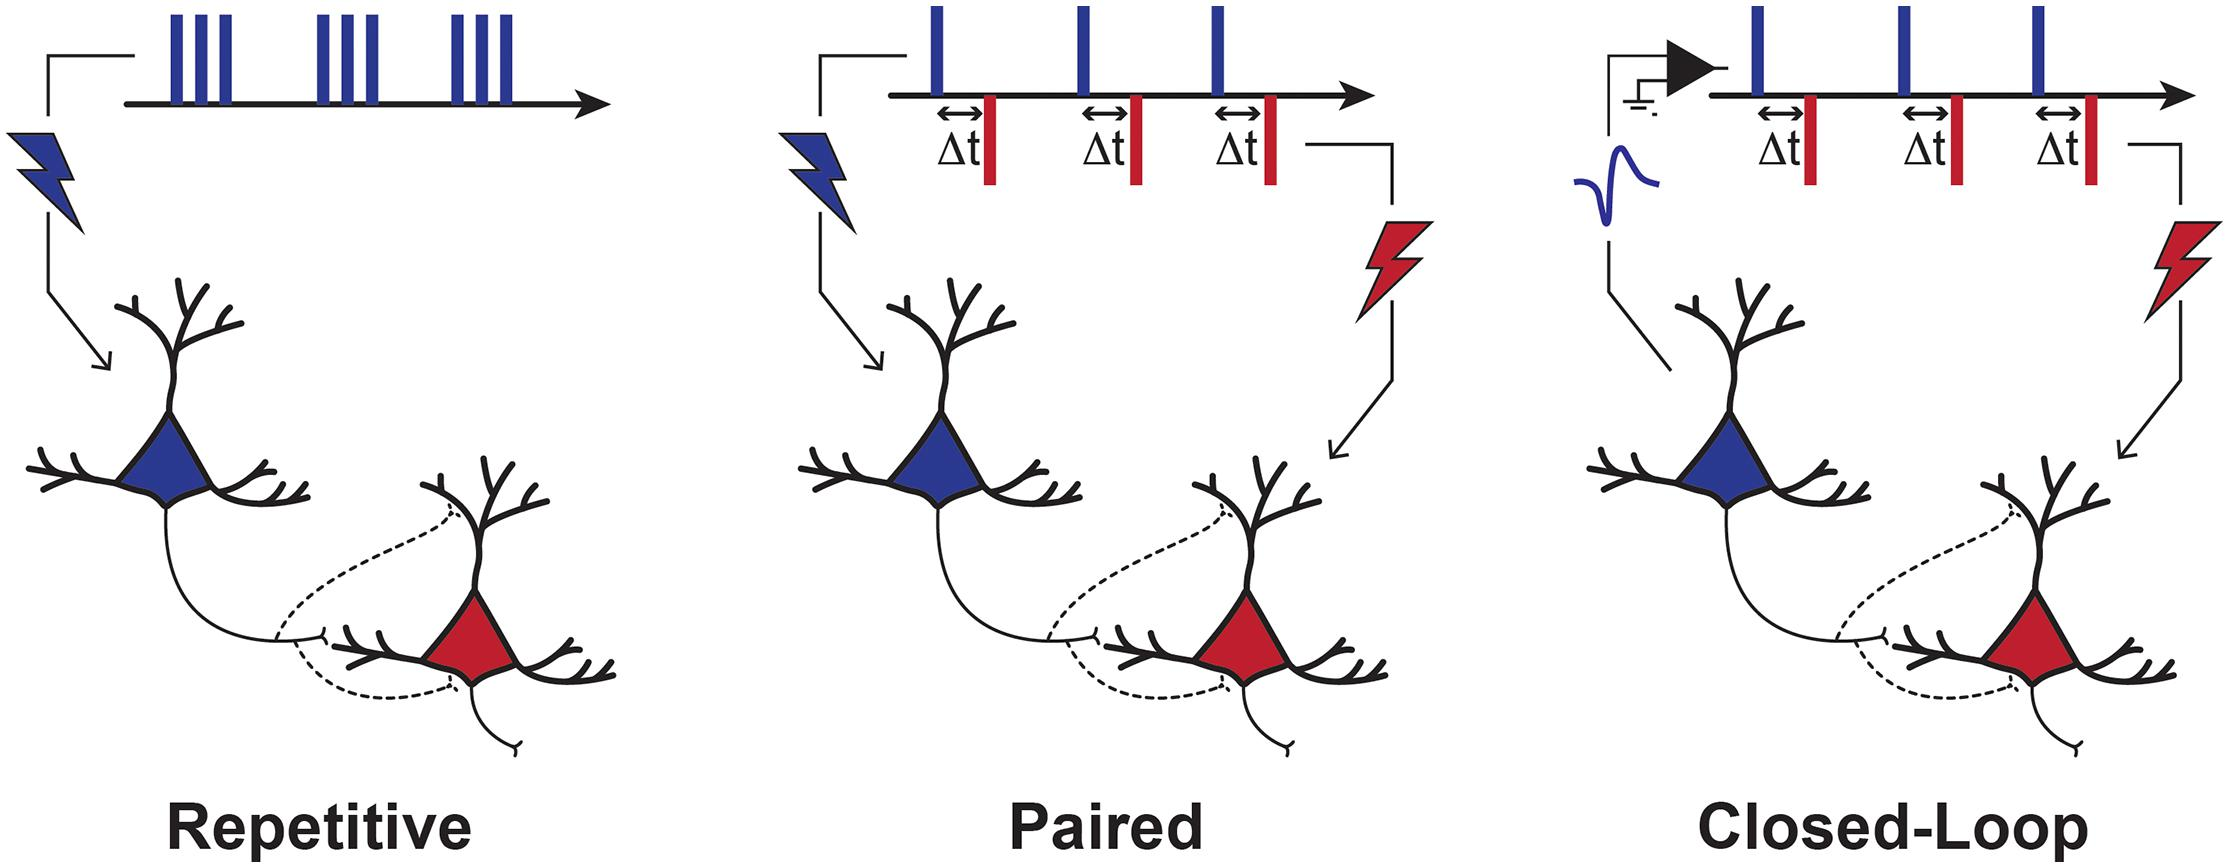
\includegraphics[width=0.9\linewidth]{Figure/Neuromodulation Paradigms.jpg}
    \end{center}
    \caption{\protect\cite{Ting2021} Stimulation paradigms to induce plasticity. Depiction of three main stimulation strategies used to induce plasticity.}
    \label{fig:Neuromodulation Paradigms}
\end{figure}

\subsubsection{Repetitive Stimulation}

Repetitive Stimulation (Figure \ref{fig:Neuromodulation Paradigms} left) involves repeatedly applying stimuli to the brain, especially to the primary motor cortex, to create lasting changes in synaptic strength and plasticity. It's often applied using non-invasive methods such as transcranial direct current stimulation (tDCS) and transcranial magnetic stimulation (TMS), with protocols like repetitive TMS (rTMS) and theta burst stimulation (TBS).

These methods tweak cortical excitability and restore a balanced interhemispheric inhibition. However, they have limitations in terms of spatial precision, and changes in cortical excitability may not always lead to long-term functional improvements. This can compromise their overall effectiveness, especially in cohorts with inter-individual variability \cite{Ting2021}.

\subsubsection{Paired Stimulation} 

Paired Stimulation (Figure \ref{fig:Neuromodulation Paradigms} center), as seen in methods like Paired Associative Stimulation (PAS) \cite{Alder2019}, synchronizes perisynaptic neuronal activity using a combination of TMS over the motor cortex and non-invasive electrical stimulation of the spinal cord or peripheral nerves. 

This method aims to modulate cortical excitability and induce spike-timing-dependent plasticity. However, the effectiveness of paired stimulation varies among subjects, requiring a deeper understanding of the brain's state to achieve precise temporal coordination during stimulation and induce plasticity \cite{Ting2021}.

\subsubsection{Closed Loop Stimulation}

Given the intricate and diverse organization of the nervous system, employing more precise stimulation techniques may prove more effective in inducing plasticity and, concurrently, lead to neural reorganization with greater functional benefits.

Closed loop stimulation paradigm (Figure \ref{fig:Neuromodulation Paradigms} right) represents a promising avenue in this regard, where the delivery of neural stimulation is dynamically adjusted based on real-time monitoring of ongoing brain activity. 
Unlike open loop approaches, closed loop stimulation systems can detect specific neuronal events or brain states and tailor the timing and intensity of stimulation accordingly. This refinement, for example in the  Deep Brain Stimulation (DBS), contributes to enhanced precision, efficacy, and overall functional benefits.
Both Behavior-Controlled stimulation and EEG-Controlled stimulation infer voluntary effort, but the latter doesn’t depend on physical movement. However, while offering advantages through adaptability and precision in enhancing natural patterns of neuronal and muscular activity in stroke patients, limitations in effectiveness persist for non-moving or atypical patients.
Closed loop stimulation can be employed in therapeutic neuroprostheses and Brain-Computer Interfaces (BCI), also using invasive methods. Studies have shown that spike-triggered intracortical stimulation is effective in improving functional recovery, reactivating paralyzed muscles, and inducing plasticity \cite{Ting2021}.

Nevertheless, despite recent results demonstrated the capabilities of a personalized closed loop approach (called Activity Dependent Stimulation, ADS), to better entrain network activity compared to standard open loop random stimulation \cite{Guggenmos2013,Averna2020,Averna2021}, the deployment of closed loop systems, whether invasive or non-invasive, is hindered by technical complexities and restricted accessibility.
 
\subsection{Neuroprostheses}

Neuroprosthetics represent a cutting-edge field at the intersection of neuroscience, engineering, and medical technology concerned with developing prosthetic devices that interact with the nervous system. 
These bioelectronic devices can also be classified as bio-hybrid systems, considering the human factor as a biological component, and they can be implemented using both open loop and closed loop approaches.

These neuroprostheses aim to substitute or regulate portions of the nervous system where electrophysiological activity has been disrupted due to neurodegenerative and neuropsychiatric disorders, after stroke, Traumatic Brain Injury (TBI), or Spinal Cord Injury (SCI).
They are currently employed to treat motor and sensory disorders, but lately, cognitive deficits have also become a target \cite{Gupta2023}.

Recent advancements have led to the development of closed loop neuromorphic neuroprostheses \cite{Famm2013,Reardon2014}, capable of establishing bidirectional communication between the artificial and biological components \cite{Broccard2017} and delivering output through electrical, chemical, or optogenetic stimulation \cite{Christensen2022}.

Indeed, a closed loop architecture is essential for developing a neuroprosthesis \cite{Levi2018,Buccelli2019}, specifically a type known as brain-prostheses. These brain-prostheses are designed to replicate the electrical activity of biological neural networks, facilitating interaction between the artificial and biological components \cite{Bonifazi2013}. They also enable the replacement of a damaged brain area with an artificial device capable of providing an interpretable response to the nervous system after processing the acquired neural signals.

\begin{figure}[ht!]
    \begin{center}
    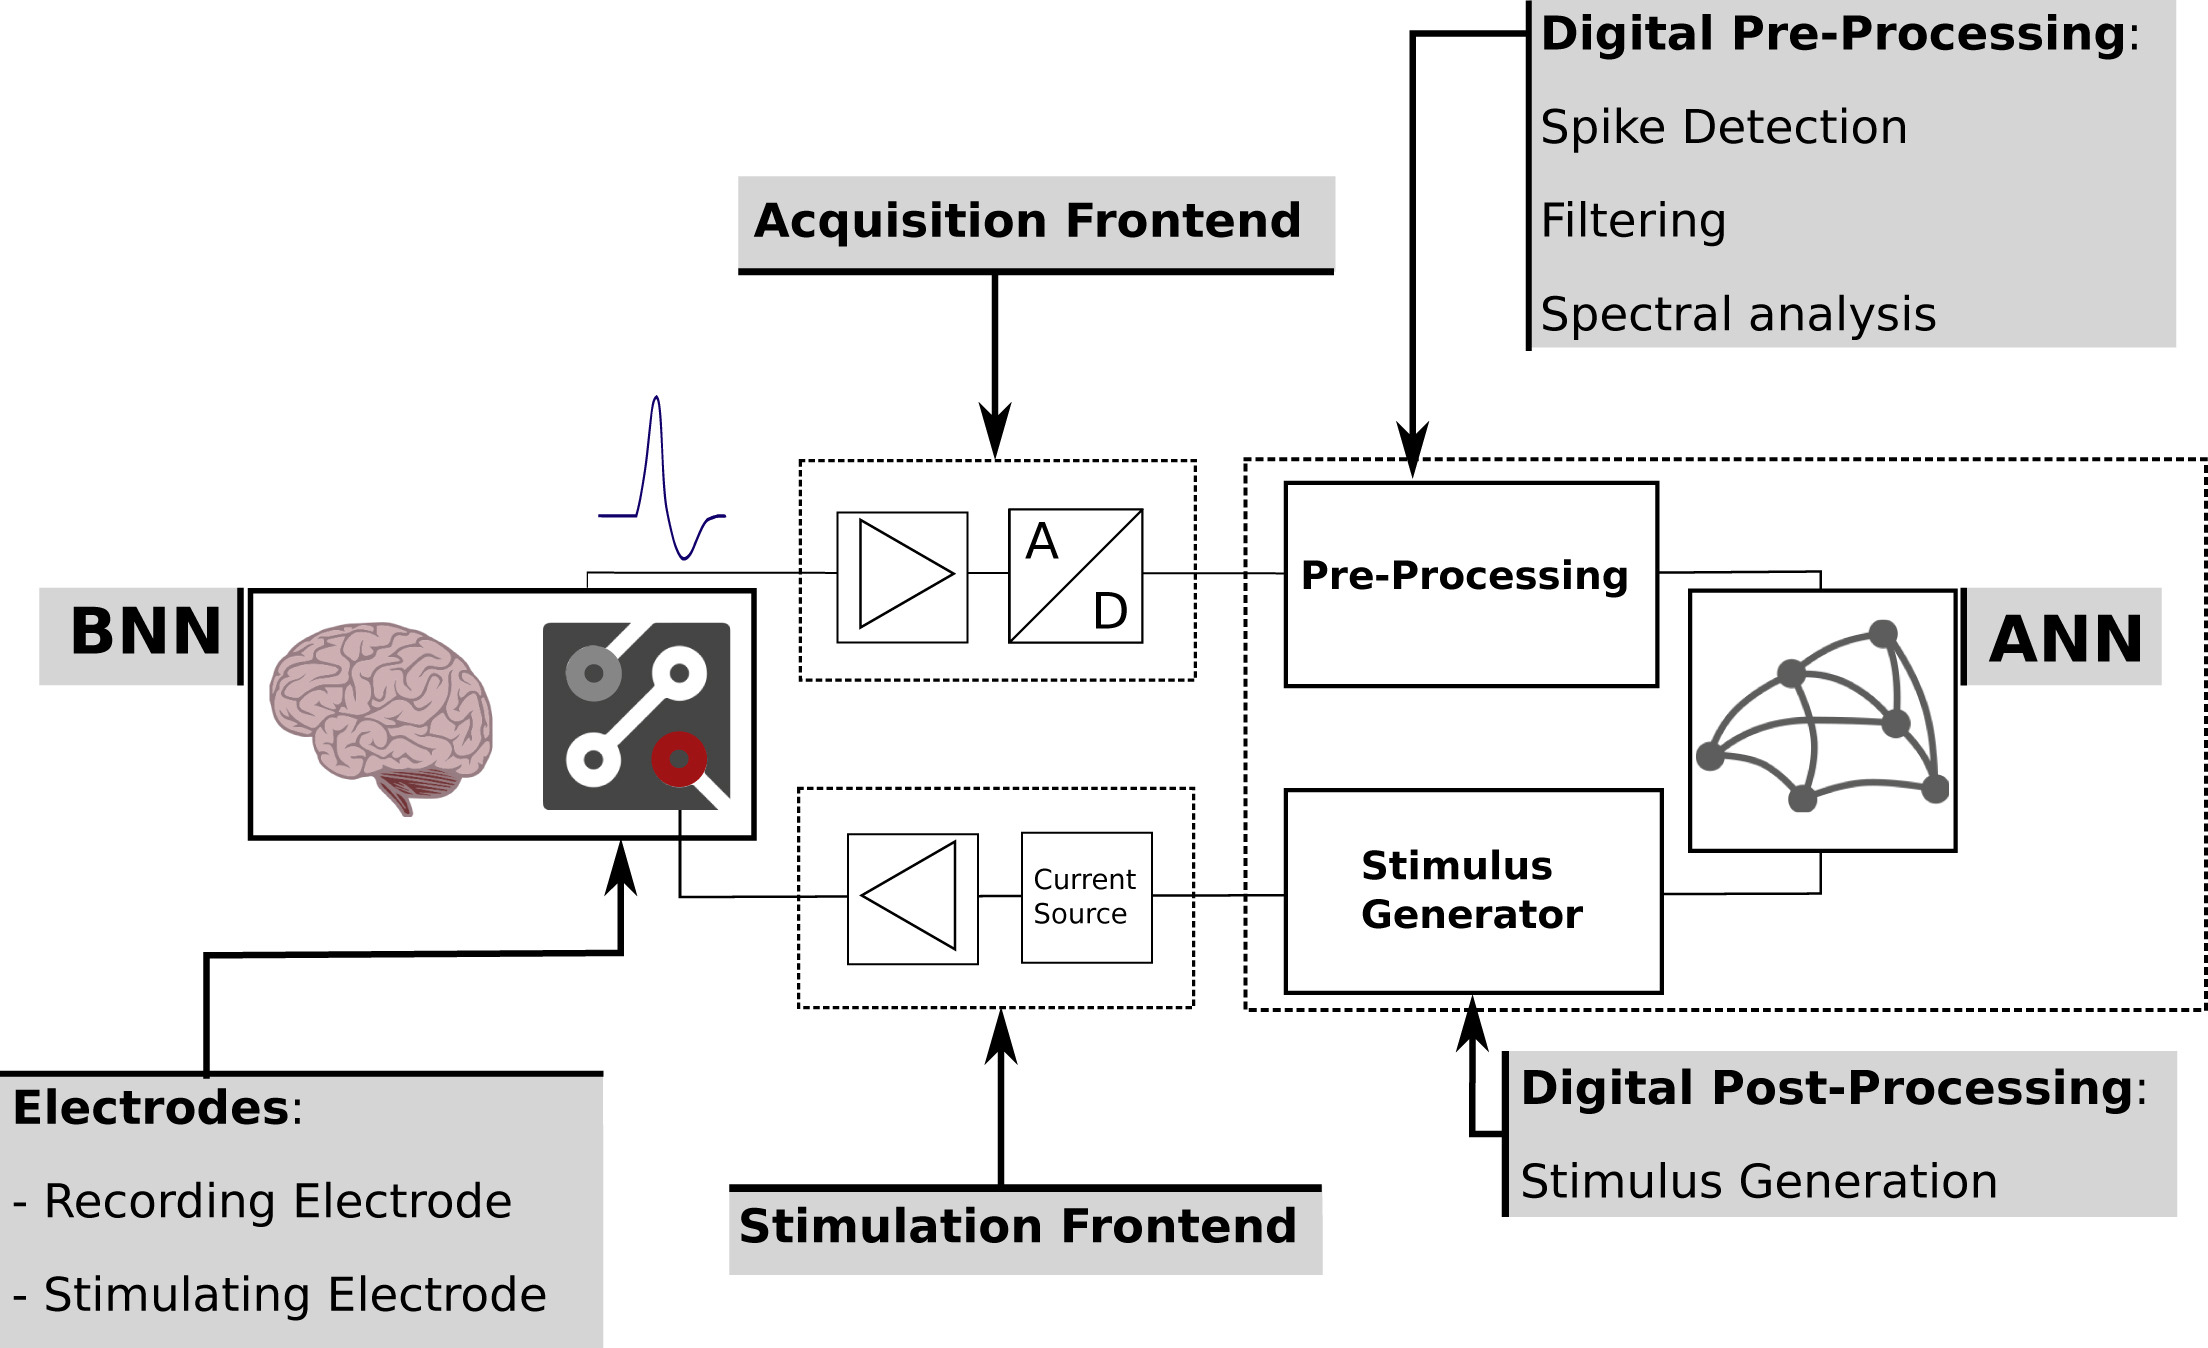
\includegraphics[width=0.9\linewidth]{Figure/Bio-Hybrid Closed Loop System.jpg}
    \end{center}
    \caption{\protect\cite{George2020} Setup of a bio-hybrid closed loop system. The Biological Neural Network (BNN) and the Artificial Neural Network (ANN) are connected through stimulation and recording electrodes. The BNN activity is amplified and digitized before extracting informative features, which are then fed as input into the ANN. Then, the ANN activity defines the stimulation protocol to be applied to the BNN through the stimulation electrodes. This mutual influence creates a bidirectional communication.}
    \label{fig:Bio-Hybrid Closed Loop System}
\end{figure}

As depicted in Figure \ref{fig:Bio-Hybrid Closed Loop System}, the neuromorphic artificial component of the bio-hybrid system can consist of an Artificial Neural Network (ANN) that simulates the architecture and complex dynamics of biological neurons.\\
These ANNs can be of two types: bio-inspired or bio-mimetic. The former category includes computational systems inspired by biological architectures that use simplified neuron models, for example, to execute accelerated time simulations in the field of artificial intelligence \cite{Tavanaei2019}. The latter category includes realistic models that imitate biological neurons and faithfully reproduce their features using complex neuron models operating at biological timescales. These models are employed to simulate neural network dynamics and/or conduct bio-hybrid experiments.

In the family of ANNs, Spiking Neural Networks (SNNs) are the most biophysically plausible, as they can reproduce neuronal phenomena, ranging from electrophysiological activity in single cells (soma, axon, and dendrites) to the plasticity of the network. By integrating bio-mimetic with multi-compartment models, it becomes possible to model also the morphological characteristics of a neuron and design an SNN capable of reproducing the spatial configuration of neurons and associated spike timing and morphology.

Recently, a biomimet\-ic Spiking Neural Network (SNN) has been utilized to develop an electroceutical solution \cite{DiFlorio2023} that, in contrast to \cite{Buccelli2019}, employed Hodgkin-Huxley neurons. The SNN, consisting of 1024 unconnected neurons, dictated the pace for open-loop stimulation to the brains of rats as part of a post-stroke rehabilitation protocol.

Most of the current solutions for biomimetic SNN simulations are soft\-ware-based, such as NEURON, NEST, and Brian2 \cite{HinesCarnevale2001,GewaltigDiesmann2007,Stimberg2019}, and they are not suited for real-time emulation and interaction at the biological timescale due to the high computational time required.

On the contrary, hardware-based SNNs, such as TrueNorth, BrainScaleS-2, SpiNNaker, and Loihi \cite{Merolla2014,Pehle2022,Painkras2013,Davies2018,Stradmann2022}, are able to perform real-time emulation and can be either analog, hence less power-hungry, or digital, hence more flexible and more suited for prototyping.

This work focuses on tuning the parameters of a new real-time hardware-based SNN, Bi{\oe}muS \cite{Beaubois2023}, to be used for delivering novel personalized electrical stimulations in pre-clinical studies.

\section{Biological Modeling}

Models are frequently employed across various disciplines to explore intricate problems, offering a means to circumvent constraints and external influences. Specifically, biological models of the human body serve as experimental systems designed to replicate specific biological processes both physiological and pathological. These models generally fall into two categories: in-vitro (cell-based) and in-vivo (animal-based).

\subsection{In-vitro 2D models}

In-vitro two-dimensional (2D) cultures are cellular models cultivated on flat surfaces, such as culture dishes or multi-well plates, allowing for consistent control of the environment outside of a living organism. The advantage of this method lies in the simplicity of its handling and experimental measurement processes, providing a wide range of established cell lines. Furthermore, it offers simplified and highly reproducible systems to investigate cellular and molecular interactions. However, this model is often limited in terms of physiological coherence, as it does not fully reproduce the complexity of tissues and organs.

\subsection{In-vitro 3D models}

In-vitro three-dimensional (3D) cultures are cellular models cultivated in a device that allows cells to organize and interact in three dimensions, thereby replicating tissues and organs in a more coherent manner \cite{Pampaloni2007,BreslinO’Driscoll2013,Duval2017}. 

For example, in-vitro 3D cultures are widely used to study the human brain, such as through organoid cultures that can reproduce structures of certain brain areas \cite{Kim2020}.

A more complete model involves the design of Organ-On-Chip (OOC) systems, which are microfluidic platforms incorporating cells and tissues in a three-dimensional arrangement to replicate, in vitro, the complex architecture and interactions present in real human organs \cite{Huh2011,Ma2021}.

\subsection{In-vivo models}

In-vivo models for human biology modeling often involve animals, such as rodents \cite{Peters2007} and non-human primates. To date, they are of fundamental importance for future applications in humans. These experiments explore various biological processes, diseases, and drug responses within the authentic physiological context of living organisms, exhibiting fewer limitations compared to in-vitro cultures.

While in-vivo experiments account for the complex interactions in a living organism, thus providing a more coherent approach, they are often significantly more complex to conduct compared to in-vitro 2D experiments. Notably, in-vivo studies demand rigorous adherence to ethical protocols to ensure both animal welfare and the scientific integrity of the research conducted.

\subsubsection{In-vivo models of Stroke}

Various rodent models are employed for testing neuroprotective therapies and exploring reparative mechanisms in the brain post-stroke. These models aim to create reproducible infarcts with minimal surgical intervention to decipher cell death mechanisms and assess neuroprotective strategies. Ischemic stroke animal models are broadly categorized as global, focal, and multifocal \cite{Graham2004}:
\begin{itemize}
    \item In cases of global ischemia, there is a reduction in blood flow across the entire brain. It can be complete, involving the total cessation of global blood flow for a period, or incomplete, entailing a significant reduction in blood flow to impede normal metabolism and function;
    \item Focal strokes target specific brain regions and are prominently represented by middle cerebral artery occlusion (MCAO), where a blood clot is introduced through the internal carotid to occlude the MCA, temporarily or permanently reducing blood flow to a specific hemisphere. This model closely mimics human ischemic stroke \cite{Garcia1993,Tsuji2013,Zhang2013}. Other methods, such as the stereotaxic injection of the vasoconstrictive peptide endothelin-1 (ET-1) into the cortex, precisely localize effects to specific brain regions, supporting functional recovery \cite{Frost2006,Fang2010};
    \item Multifocal ischemic strokes induce reduced cerebral blood flow in multiple areas using various methods such as embolization, microspheres, or photochemically induced thrombi \cite{McAuley1995,Traystman2003}.
\end{itemize}

In this work, a rodent model of focal ischemic stroke induced by ET-1 was employed. This method is known for being less invasive, having low mortality, and inducing direct focal ischemia in both deep and superficial brain regions \cite{Sharkey1993}. The lesion was performed in the caudal forelimb area (CFA), a region within the cortical sensorimotor system. 

This area in the frontal cortex shares many characteristics with the primary motor cortex (M1) of primates, and injuries to M1 are known to lead to long-term impairments in reaching and grasping functions \cite{Nishibe2010}. Traditionally, it was believed that such impairments occurred because M1 provides substantial outputs to the motor apparatus in the spinal cord, directly affecting motor output function. However, M1 also has significant interconnections with the primary somatosensory cortex (S1) located in the parietal lobe (Figure \ref{fig:Brain-Machine-Brain Interface}A). Long-range corticocortical fibers from S1 play a crucial role in providing information to M1 regarding the limb's position in space. Consequently, impaired motor performance resulting from an injury to M1 could be also attributed, at least partially, to a disruption in communication between the somatosensory and motor cortex \cite{Friel2005}.

\begin{figure}[ht!]
    \begin{center}
    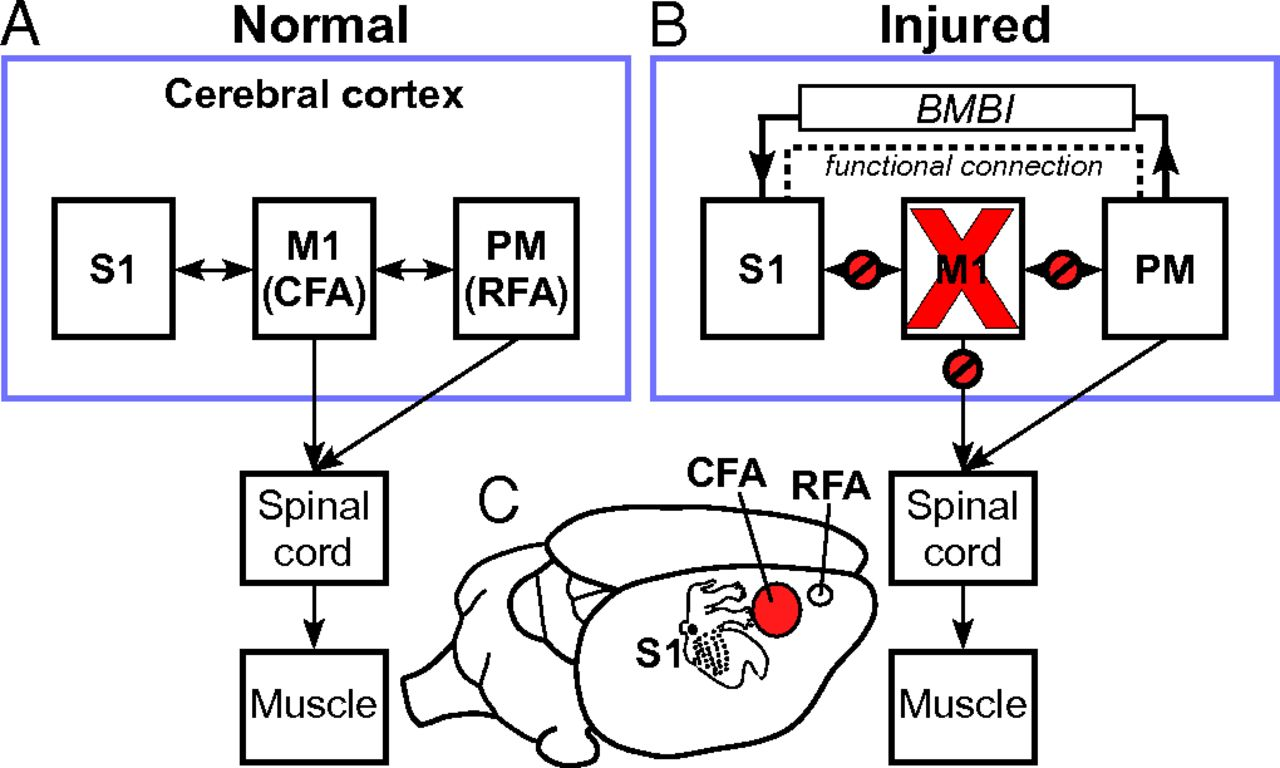
\includegraphics[width=0.9\linewidth]{Figure/Brain-Machine-Brain Interface.jpeg}
    \end{center}
    \caption{\protect\cite{Guggenmos2013} Theoretical model of neuroprosthetic treatment approach after brain injury. (A) Normal connectivity of M1, S1, and PM. Both M1 (CFA in rat) and PM (RFA in rat) send substantial outputs to the spinal cord via the corticospinal tract. Also, extensive reciprocal connections exist between M1 and PM, as well as between M1 and S1. (B) Effects of focal M1 injury on brain connectivity and the hypothetical effect of a BMBI to restore somatosensory-motor communication. An injury to M1 disrupts the corticocortical communication between M1 and S1 (and between M1 and PM). Thus, the uninjured PM, which contains corticospinal neurons as well, might be exploited. The dotted line indicates enhanced functional connection between PM and S1 established after treatment with a BMBI.(C) Location of target areas in rat cerebral cortex. A topographic map of the somatosensory representation in S1 is superimposed on the cortex.}
    \label{fig:Brain-Machine-Brain Interface}
\end{figure}

In particular, the rostral forelimb area (RFA) is believed to contribute to the recovery of function after an injury to M1 \cite{Nishibe2010,Conner2005,Rouiller1993}, and it was indeed exploited in \cite{Guggenmos2013} for the development of a closed-loop brain–machine–brain interface (BMBI)(Figure \ref{fig:Brain-Machine-Brain Interface} B,C). The RFA is a premotor region in the rodent's frontal cortex that shares many characteristics with the premotor (PM) cortex of primates. Although PM areas also have long-range corticocortical connections with somatosensory areas, in intact animals, these connections appear to be relatively weak compared to M1's connections with the somatosensory cortex \cite{Rouiller1993,Dancause2005,Fang2005}.

\section{Artificial Modeling}

Artificial models, inspired by nature, play a crucial role in simplifying and simulating specific aspects of systems, addressing technological challenges across various fields. Bio-inspired Artificial Neural Networks (ANNs), emulating the architecture of the human brain, excel in diverse signal processing tasks. Image recognition, classification, natural language processing, speech recognition, and time-series prediction tasks often leverage Feedforward Neural Network (FNN) \cite{Svozil1997}, Convolutional Neural Network (CNN) \cite{O'SheaNash2015}, or Recurrent Neural Network (RNN) \cite{MedskerJain1999} for information processing. Additionally, SNNs, introduced in the section "Neuroprosthesis", represent a more biologically accurate form of ANNs, simulating the behavior of biological neurons and their interactions through action potentials or spikes \cite{Ghosh-DastidarAdeli2009}.

\subsection{Neuron models}

Differently from the mere bio-inspired neurons used in artificial intelligence (for FNN, CNN and RNN), bio-mimetic neurons aim to faithfully reproduce phenomena happening in nature.

The model proposed by \cite{HodgkinHuxley1990}, known as the HH model, is considered the first biologically meaningful mathematical neuron model. Derived from experiments conducted on the squid giant axon, this model incorporates three currents: sodium, potassium, and leak current. The experiments revealed that the ionic permeability of the membrane is highly dependent on the membrane potential. As a result, the HH model was developed based on the voltage-dependent properties of the membrane to simulate the generation of an action potential. The opening and closing of ion channels are represented as variable conductance determined by the voltage.

Figure \ref{fig:HH model Electric Circuit} depicts the schematic of the Hodgkin-Huxley model whose behaviour is described by the Equation \ref{eq:HH model}.

\begin{figure}[ht!]
    \begin{center}
    \begin{circuitikz}
    \draw (3,-3) node[circle, fill=black, draw, inner sep=1pt]{};
    \draw (3,-3) node[below] {Intracellular};
    \draw (3,-3) -- (3,-2);
    \draw (3,3) node[circle, fill=black, draw, inner sep=1pt]{};
    \draw (3,3) node[above] {Extracellular};
    \draw (3,3) -- (3,2);
    \draw (0,-2) -- (6,-2);
    \draw (0,2) -- (6,2);
    
    % Capacitor
    \draw (6,2) to[C, l=$C_m$] (6,-2);

    % Sodium branch
    \draw (0,0) to[vR, l=$g_{Na}$] (0,2);
    \draw (0,-2) to[battery1] (0,0);
    \draw (-0.90,-1.3) node[circle, label=$E_{Na}$, inner sep=1pt]{};
    
    % Potassium branch
    \draw (2,0) to[vR, l=$g_{K}$] (2,2);
    \draw (2,-2) to[battery1, invert] (2,0);
    \draw (1.10,-1.3) node[circle, label=$E_{K}$, inner sep=1pt]{};

    % Leak branch
    \draw (4,0) to[R, l=$g_{Leak}$] (4,2);
    \draw (4,-2) to[battery1, invert] (4,0);
    \draw (3.10,-1.3) node[circle, label=$E_{Leak}$, inner sep=1pt]{};

    \draw [>=stealth, <->] (8,-3) -- (8,3);
    \draw (8.4,-0.3) node[above] {$V_{m}$};

    \end{circuitikz}
    \end{center}
    \caption{Electrical equivalent circuit of HH model representing $Na^{+}$, $K^{+}$ ionic currents and leakage current as a basic neuron model. $V_{m}$ is the membrane potential, $C_{m}$ is the membrane capacitance, $g_{Na}$ and $g_{K}$ the conductance of voltage-dependent ion channels, $E_{Na}$, $E_{K}$ and $E_{Leak}$ are the reversal potentials and $g_{Leak}$ a voltage independent conductance.}
    \label{fig:HH model Electric Circuit}
\end{figure}

\begin{equation}
C_m \frac{dV_m}{dt}=-(I_{Na}+I_{K}+I_{Leak})
\label{eq:HH model}
\end{equation}

where $I_{Na}$ is the sodium current, $I_{K}$ the potassium current, $I_{Leak}$ the leakage current.

Due to the complexity of the HH model, which relies on high-dimensional nonlinear differential equations, simpler models have been developed. These simplified models replicate neural dynamics using reduced equations, often incorporating threshold and reset mechanisms to generate action potentials.

Both FitzHugh-Nagumo [FitzHugh, 1955, FitzHugh, 1961, Nagumo et al., 1962] and Morris-Lecar [Morris and Lecar, 1981] models reduce the number of variables and equations compared to the HH model, capturing essential features of excitable cells while sacrificing some biophysical accuracy. These simplifications make FitzHugh-Nagumo and Morris-Lecar models suitable for certain applications where computational efficiency is crucial and detailed biophysical accuracy is not essential. 

Even further simplification of neuronal dynamics is found in the family of Integrate-and-Fire (IF) models  \cite{Abbott1999}. In the IF model, a spike is generated each time the membrane potential crosses the threshold, and it is reset to the resting potential only after this event. The family includes variations like Leaky Integrate-and-Fire (LIF) \cite{GerstnerKistler2002}, Exponential Integrate-and-Fire (EIF) \cite{Fourcaud-Trocmé2003}, and Adaptive Exponential Integrate-and-Fire (AdEx) \cite{GerstnerBrette2009} models that introduce specific modifications to enhance biological plausibility while maintaining computational efficiency.

A model with significantly better biological plausibility is the Izhikevich (IZ) model \cite{Izhikevich2003}, capable of reproducing various neuron families (as illustrated in Figure \ref{fig:Izhikevich Spiking Neuron Families}), while remaining computationally convenient.

\begin{figure}[ht!]
    \begin{center}
    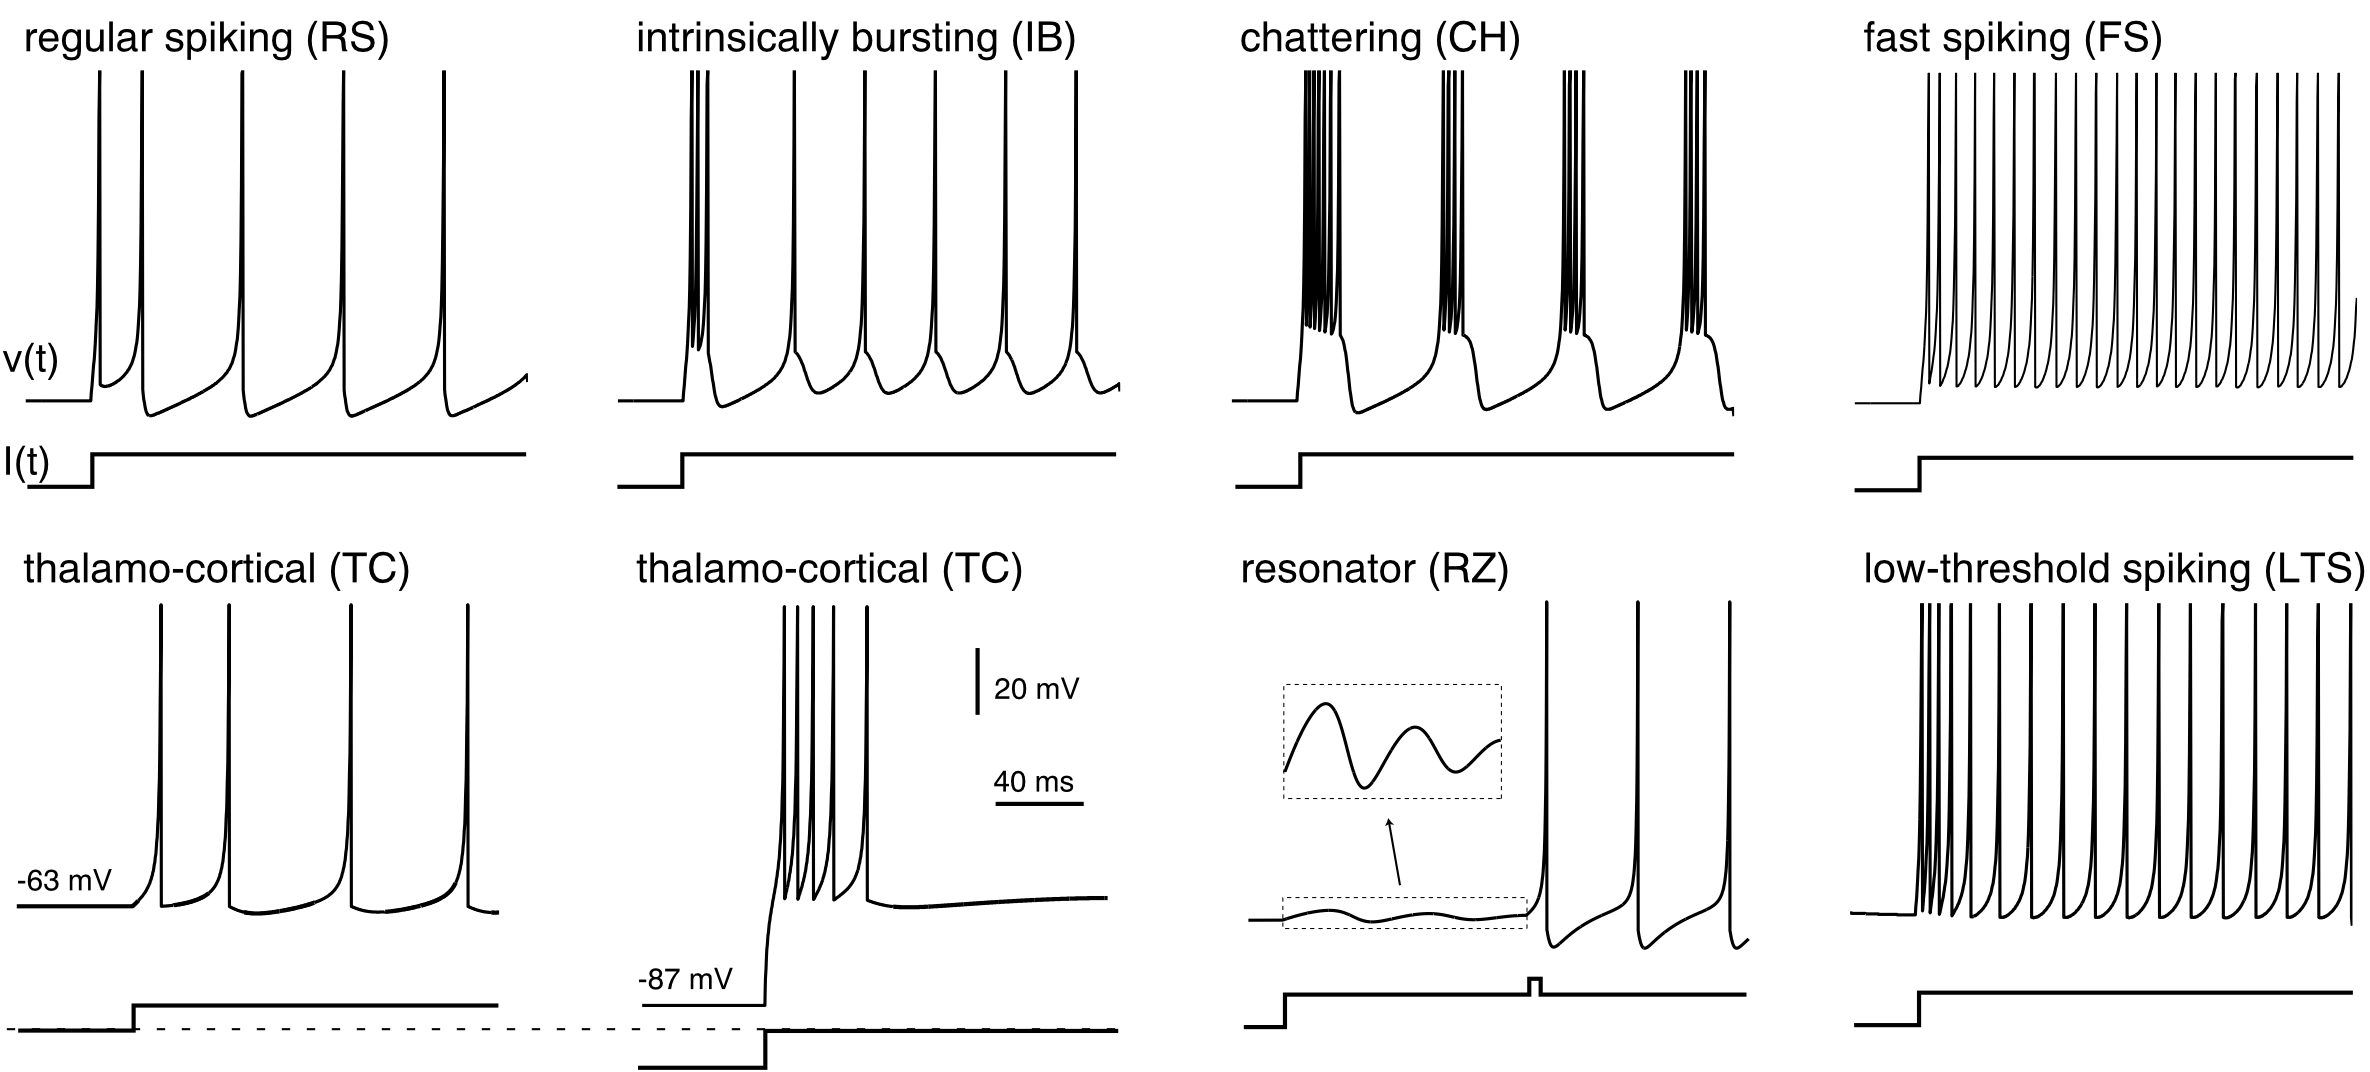
\includegraphics[width=0.9\linewidth]{Figure/Izhikevich Spiking Neuron Families.jpg}
    \end{center}
    \caption{\protect\cite{Izhikevich2003} Spiking neuron families obtained using different values of the parameters in the Izhikevich model.}
    \label{fig:Izhikevich Spiking Neuron Families}
\end{figure}

However, while biophysical meaningfulness is a critical requirement for true bio-mimetic modeling, the implementation on a numeric platform introduces a dilemma between biological coherence and practicality. Despite the IZ model presenting an appealing compromise between implementation cost and biological coherence, it lacks biological meaningfulness and deviates from bio-realism, impacting its ability to predict the behavior of neurons in specific conditions \cite{Brette2015}.

In this work, the highest biological coherence and meaningfulness were achieved by utilizing a SNN with conductance-based HH neurons, representing the best bio-mimetic model.

\subsubsection{Single-compartment models}

The single-compartment model of a neuron is commonly employed in computational neuroscience, approximating the neuron to a point in space and neglecting the spatial dimension. It is represented as a large membrane capacitance in parallel with a series of conductances and batteries, as illustrated in Figure \ref{fig:HH model Electric Circuit}. The temporal dynamics of the membrane potential, capturing the essential mechanisms of $Na^{+}$ and $K^{+}$ channels, can be described using the HH model by Equation \ref{eq:HH model}.

More specifically, each ionic current can be represented by Equation \ref{eq:General Ion Current}:

\begin{equation}
I_{ion} = g_{ion} m^{{p}_{ion}}_{ion} h^{{q}_{ion}}_{ion} (V-E_{ion})
\label{eq:General Ion Current}
\end{equation}

where $I_{ion}$ is the ionic current, $g_{ion}$ is the maximum conductance of the ion channel, $m^{{p}_{ion}}$ and $h^{{q}_{ion}}$ are respectively the activation and inactivation variables, each taking a probability value between 0 and 1, $v$ is the membrane voltage and $E_{ion}$ is the equilibrium potential of the ion. 

In general, depending on the desired neuron model, several ion channels can be included. In the case represented in Figure \ref{fig:HH model Electric Circuit} and Equation \ref{eq:HH model}, three currents are considered, corresponding to Equations \ref{eq:Sodium Ion Current}, \ref{eq:Potassium Ion Current}, \ref{eq:Leakage Current}:

\begin{equation}
I_{Na} = g_{Na} m^{3}_{Na} h_{Na} (V-E_{Na})
\label{eq:Sodium Ion Current}
\end{equation}

\begin{equation}
I_{K} = g_{K} m^{4}_{K} (V-E_{K})
\label{eq:Potassium Ion Current}
\end{equation}

\begin{equation}
I_{Leak} = g_{Leak} (V-E_{Leak})
\label{eq:Leakage Current}
\end{equation}

The values of the activation and inactivation variables of the voltage-gated ion channels are described by equations representing different sigmoids for each channel. The formulae are expressed using the following formalism (Equation \ref{eq:General Gating Particle}):

\begin{equation}
\frac{dp_{i}}{dt} = \alpha_{i}(V)(1-p_{i})-\beta_{i}(V)p_{i}
\label{eq:General Gating Particle}
\end{equation}

where $\alpha$ and $\beta$ are voltege-dependent parameters. Introducing the steady-state solution: 

\begin{equation}
p_{i, t\to\infty}(V) = \frac{\alpha_{i}(V)}{\alpha_{i}(V)+\beta_{i}(V)}
\label{eq:Steady-state Solution Gating Particle}
\end{equation}

and the time constant formulae:

\begin{equation}
\tau_{i}(V) = \frac{1}{\alpha_{i}(V)+\beta_{i}(V)}
\label{eq:Time Constant Gating Particle}
\end{equation}

the Equation \ref{eq:General Gating Particle} can be written as follow:

\begin{equation}
\frac{dp_{i}}{dt} = \frac{p_{i, \infty}(V)-p_{i}}{\tau_{i}(V)}
\label{eq:Alternative General Gating Particle}
\end{equation}

\subsubsection{Multi-compartmental models}

The multi-compartmental model provides a more biologically realistic approach, enabling the analysis of complex spatial details and behaviors of neurons. In particular, it allows the investigation of biophysical phenomena and neurodegenerative diseases that affect specific regions of the neurons. 

Thus, the neuron is discretized into more or fewer compartments, depending on the desired level of fidelity or abstraction, following the cable theory. Each segment is then described by an electrical equivalent circuit, such as the HH model, linked to each other by resistors simulating axoplasmic resistance (as depicted in Figure \ref{fig:Multi-compartimental Model}).

\begin{figure}[ht!]
    \begin{center}
    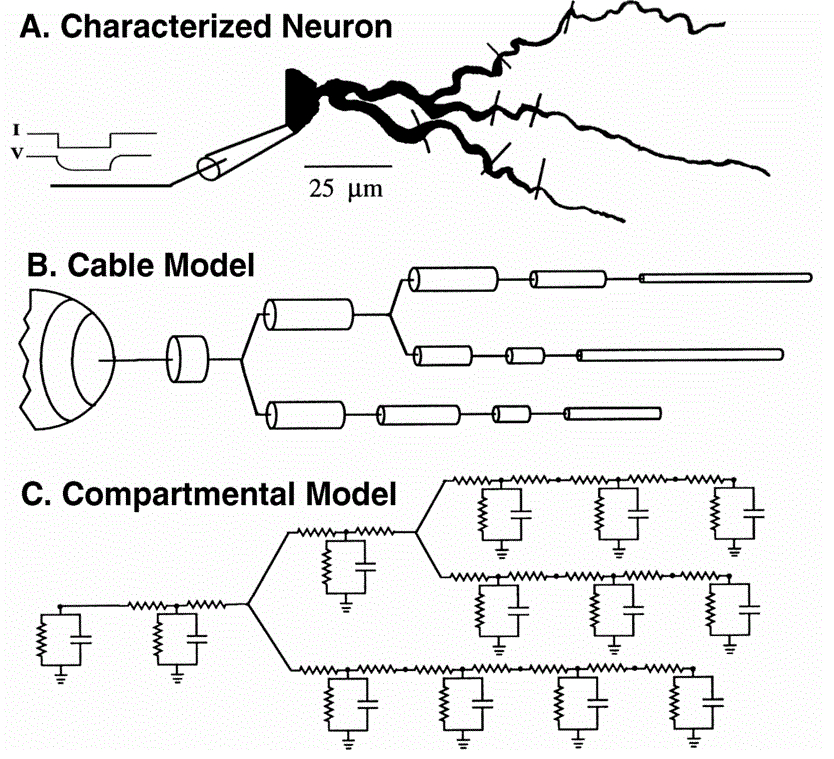
\includegraphics[width=0.9\linewidth]{Figure/Multi-compartimental Model.jpg}
    \end{center}
    \caption{Electrical equivalent circuit of multicompartmental neuron model. The neuron (A) is first discretized into cylindrical compartments of various lengths and radii (B), and then each segment is represented by its own equivalent electrical circuit (C). Extracted from [Christof Koch, Idan Segev, CC BY-SA 3.0 (https://creativecommons.org/licenses/by-sa/3.0), via Wikimedia Commons]}
    \label{fig:Multi-compartimental Model}
\end{figure}

Given that each element of the neuron corresponds to a different compartment, it's possible to describe the properties of each segment with a specific HH model. This crucial feature makes the multi-compartmental models even more biologically meaningful compared to the single-compartment models.

\subsection{Noise models}

A peculiar behaviour of the neurons is their capacity to generate spontaneous stimulus-independent spikes. Thus, is fundamental to reproduce this property in an artificial model. 

Commonly, this behavior is modeled by injecting a noisy current based on a normal distribution into the neuron, eliciting more or fewer spikes depending on its amplitude and standard deviation. However, it's possible to generate a current more similar to the synaptic noise observed in biology by fluctuating the conductances of ion channels \cite{Destexhe2001,Tuckwell2002}. Equation \ref{eq:Biomimetic Noise} expresses this biomimetic noise, which is based on the Ornstein-Uhlenbeck process.

\begin{equation}
\frac{di_{noise}(t)}{dt} = \theta(\mu-i_{noise}(t)) + \sigma\frac{dW(t)}{dt}
\label{eq:Biomimetic Noise}
\end{equation}

where $i_{noise}$ is the noisy current, $\theta$ and $\sigma$ define respectively the amplitude and deviation of the noise, $\mu$ is a constant adding drift, and $\frac{dW(t)}{dt}$ denotes the Wiener process.

\subsection{Synapse models}

Achieving a biophysically realistic model of the spike implies modeling the synapses as well. Among all the synapse models present in the literature, the one proposed by \cite{Destexhe1998} is the most biomimetic and biologically meaningful. Four types of synaptic receptors responsible for fast and slow excitation (AMPAR and NMDAR) and fast and slow inhibition (GABA\textsubscript{A}R and GABA\textsubscript{B}R) are modeled. It is a conductance-based model, and the synaptic currents generated by the receptors are expressed through Equations \ref{eq:AMPAR Synaptic Current}, \ref{eq:NMDAR Synaptic Current}, \ref{eq:GABAAR Synaptic Current} and \ref{eq:GABABR Synaptic Current}, and visualized in Figure \ref{fig:Destexhe Synaptic Models}.

\begin{equation}
I_{AMPA} = g_{AMPA} r (V-E_{AMPA})
\label{eq:AMPAR Synaptic Current}
\end{equation}

\begin{equation}
I_{NMDA} = g_{NMDA} r B(v) (V-E_{NMDA})
\label{eq:NMDAR Synaptic Current}
\end{equation}

\begin{equation}
I_{GABA_{A}} = g_{GABA_{A}} r (V-E_{GABA_{A}})
\label{eq:GABAAR Synaptic Current}
\end{equation}

\begin{equation}
I_{GABA_{B}} = g_{GABA_{B}} r \frac{s^{n}}{s^{n}+K_{d}}(V-E_{GABA_{B}})
\label{eq:GABABR Synaptic Current}
\end{equation}

where $g_{AMPA}$, $g_{NMDA}$, $g_{GABA_{A}}$, $g_{GABA_{B}}$ are the maximum conductances of the receptors, $E_{AMPA}$, $E_{NMDA}$, $E_{GABA_{A}}$, $E_{GABA_{B}}$ are the equilibrium potentials, and $r$ and $s$ are the state variables for activation and inactivation of the receptors.

\begin{figure}[ht!]
    \begin{center}
    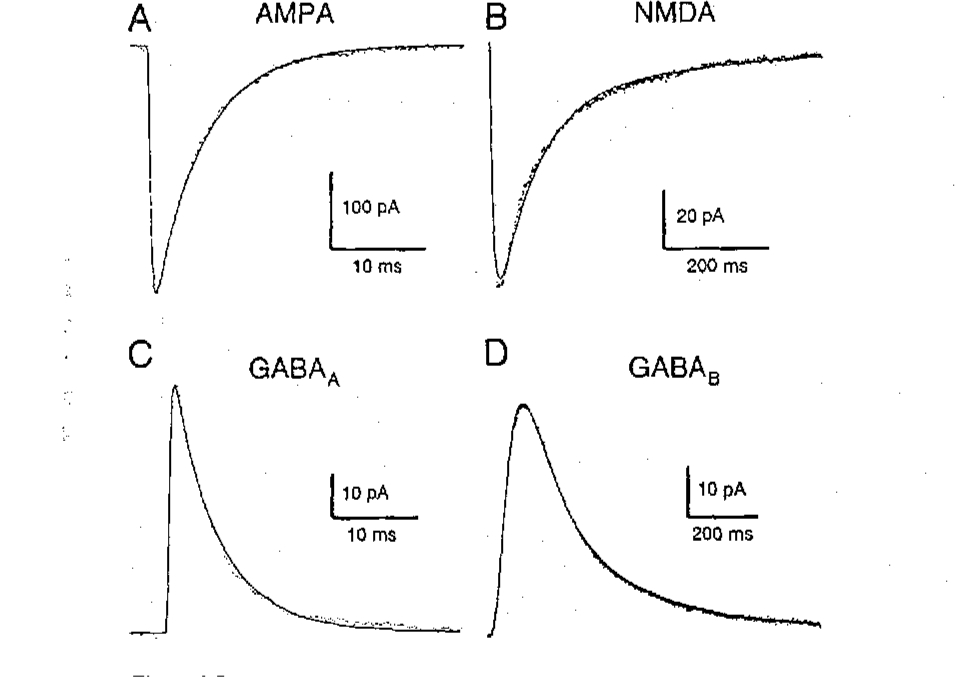
\includegraphics[width=0.9\linewidth]{Figure/Destexhe Synaptic Models.jpg}
    \end{center}
    \caption{\protect\cite{Destexhe1998} Post-synaptic currents. The curves represent the best fits of detailed kinetic models to averaged postsynaptic currents obtained from whole-cell recordings. (A) AMPAR current. (B) NMDAR current. (C) GABA\textsubscript{A}R current. (D) GABA\textsubscript{B}R current.}
    \label{fig:Destexhe Synaptic Models}
\end{figure}

For enhancing the biological fidelity and meaningfulness of the network, it's crucial to also mimic synaptic plasticity. Synaptic plasticity, in general, refers to the ability of synapses to change in strength over time and is linked to the learning capabilities of the network.

In neuroscience, Hebbian plasticity \cite{Hebb1949} is a fundamental principle that embodies the concept often expressed as "cells that fire together, wire together". This theory encompasses the most prevalent models of plasticity, including Short-Term Plasticity (STP), Spike-Timing-Dependent Plasticity (STDP), Long-Term Potentiation (LTP), and Long-Term Depression (LTD).

STP acts on short time scales (milliseconds to seconds), involving temporary increases or decreases in synaptic strength.

STDP operates over short to intermediate time scales, and the changes in synaptic strength are determined by the relative timing of spikes in pre- and postsynaptic neurons.

LTP and LTD mechanisms act on extended time scales. LTP results in a lasting reinforcement of synaptic connections induced by their repeated activation, contributing to memory formation. On the other hand, LTD leads to a weakening of synaptic connections when they are subjected to prolonged low-frequency stimulation or inactivity. This process plays a crucial role in homeostatic regulation, preventing excessive excitation caused by LTP.

\section{Summary}

This chapter introduces the main problems that the nervous system can face and the primary rehabilitation solutions to enhance stroke damage. It also covers the methods used to study the human nervous system, ranging from biological models to artificial ones. All this knowledge is essential for creating novel electroceutical treatments to deliver personalized stimulations.

The following chapters aim to delve into the steps performed in order to create a real-time hardware-based SNN that mimics the electrophysiological behavior of an in vivo Biological Neural Network (BNN). In particular, the next chapter will focus on characterizing the evoked activity, which will be used to study the effects of the lesion and traditional stimulation paradigms.


\newpage
\chapter{Characterizing the interplay between RFA and S1 areas}

\section{Introduction}

When damage occurs to the brain, a disconnection often arises between two previously interconnected brain regions. Specifically, if the primary motor cortex (M1) is damaged, communication with the primary somatosensory cortex (S1) and the spinal cord is disrupted, leading to various impairments. The current standard of care for post-stroke rehabilitation relies on physical therapy. However, emerging electroceutical techniques show promise for restoring lost function by exploiting neural plasticity \cite{Carè2024}.

To evaluate the effectiveness of existing neuromodulation therapies and a novel approach, it is essential to investigate the activity of the RFA and S1 areas. This chapter will show the analyses conducted to understand how the interaction between these spared regions is influenced by an ischemic lesion in the primary motor area (M1, CFA in rats) and subsequent neurostimulation effects. It is crucial to determine whether a new relationship is established between disconnected areas, thereby restoring their communication.

\section{Materials and Methods}

\subsection{Animals}

A total of twenty-six adult male Long-Evans rats (weight: 300-400g, age: 3-4 months; Charles River Laboratories, Calco, LC, Italy) were used in this study. The rats were divided into two main categories: animals with lesions (Lesioned; N=11) and controls (Naïve; N=15)(Figure \ref{fig:Experimental Protocol}). Throughout the entire experimental timeline, the animals were anesthetized. They were randomly assigned to the following groups: (i) Naïve-Sham (animals that did not receive any lesion or stimulation, N=2), (ii) Naïve-Open Loop (animals without lesions that underwent a session of intracortical therapeutic stimulation, N=10), (iii) Lesioned-Open Loop (animals with lesions that underwent a session of Open Loop intracortical therapeutic stimulation, N=11), and (iv) Naïve-Closed Loop (animals without lesions that underwent a session of Closed Loop intracortical therapeutic stimulation, particularly Activity-Dependent Stimulation (ADS), N=3)(Figure \ref{fig:Experimental Protocol}). Animals assigned to the Open Loop treatment randomly received one stimulation type between Exponential, Repeated, and Shuffled. The experimental procedures were conducted at the Animal Facility of the Italian Institute of Technology (IIT), Genova, Italy. The Italian Ministry of Health and Animal Care (Italy: authorization ID 509/2020-PR) approved all experiments conducted in this study.

\subsection{Surgical Procedure}

Anesthesia was induced by placing the rat into a vaporizing chamber and administering gaseous isoflurane (5\% at 1 lpm). Surgical anesthesia was achieved by injecting ketamine (80-100 mg/kg IP) and xylazine (5-10 mg/kg). Anaesthesia was maintained throughout the entire surgical procedure and the registration/stimulation session with repeated bolus injections of ketamine (10-100 mg/kg/hr IP or IM) as needed. Subsequently, the rat was securely positioned in a stereotaxic frame, and continuous monitoring of vital parameters was maintained throughout the entire procedure. The surgical process commenced with the application of lidocaine cream (a topical analgesic), followed by a midline skin incision spanning rostro-caudally between 6 mm rostral to bregma and 5 mm distal to the atlanto-occipital junction the skull. The muscles of the neck overlying the Cisterna Magna or between the upper vertebrae were reflected, and a laminectomy was successfully performed on the spinal dura, facilitating the drainage of cerebrospinal fluid (CSF) to mitigate brain edema during and after the craniotomy.

Using stereotaxic measurements \cite{Kleim2003} +3.5, +2.5 AP, and –1.25, +4.25 ML, burr holes (3 mm diameter) were carefully created over the primary somatosensory area (S1) and rostral forelimb area (RFA). Once the skull was exposed, the dura mater was removed from both burr holes to allow for the insertion of two four-shank, sixteen-contact site electrodes, placed at a depth approximately of 1500 µm (1-1.5 M$\Omega$ impedance, A4x4-3mm-100-125-703-A16, NeuroNexus)

In the lesion group (i.e., Lesion), six 0.7-mm diameter holes were drilled into the skull over the left hemisphere (contralateral to the preferred forelimb) in the area corresponding to the caudal forelimb area (CFA; the M1 forelimb representation analogue in rats) as follows: +2.5, +1.5, +0.5 AP +2.5, +3.5 ML from bregma.
An ischemic injury was then induced in CFA by intraparenchymal injection of Endothelin-1 (ET-1; Merk Life Science S.r.l., Italy, 0.3 µg ET-1 dissolved in 1 µl saline or 1 mg ET-1 dissolved in 3.33 ml saline), a potent vasoconstrictor, 1.5 mm below the pial surface in each of the 6 holes over CFA \cite{Gilmour2005}. The spread of ET-1 with this procedure is confined to an area of 0.5 mm diameter; injections were placed to produce a continuous CFA infarct while leaving RFA and S1 intact \cite{Fang2010}.

\subsection{Experimental Protocol}

As described in the Animals section, four main experimental groups were used: (i) Naïve-Sham, (ii) Naïve-Open Loop, (iii) Lesion-Open Loop and (iv) Naïve-Closed Loop. 

The experimental timeline (Figure \ref{fig:Experimental Protocol}) mainly comprised three recording phases: before the lesion (PreL), between the lesion and stimulation (PoL), and after the stimulation (PoS). The first phase included a sequence of 20-minute spontaneous activity, 10-minute connectivity mapping, and another 10-minute spontaneous activity recordings. The second phase consisted of 20-minute spontaneous activity recording followed by 10-minute connectivity mapping recording. The final phase comprised 10-minute connectivity mapping recording followed by 20-minute spontaneous activity recording.

\begin{figure}[htp]
    \begin{center}
    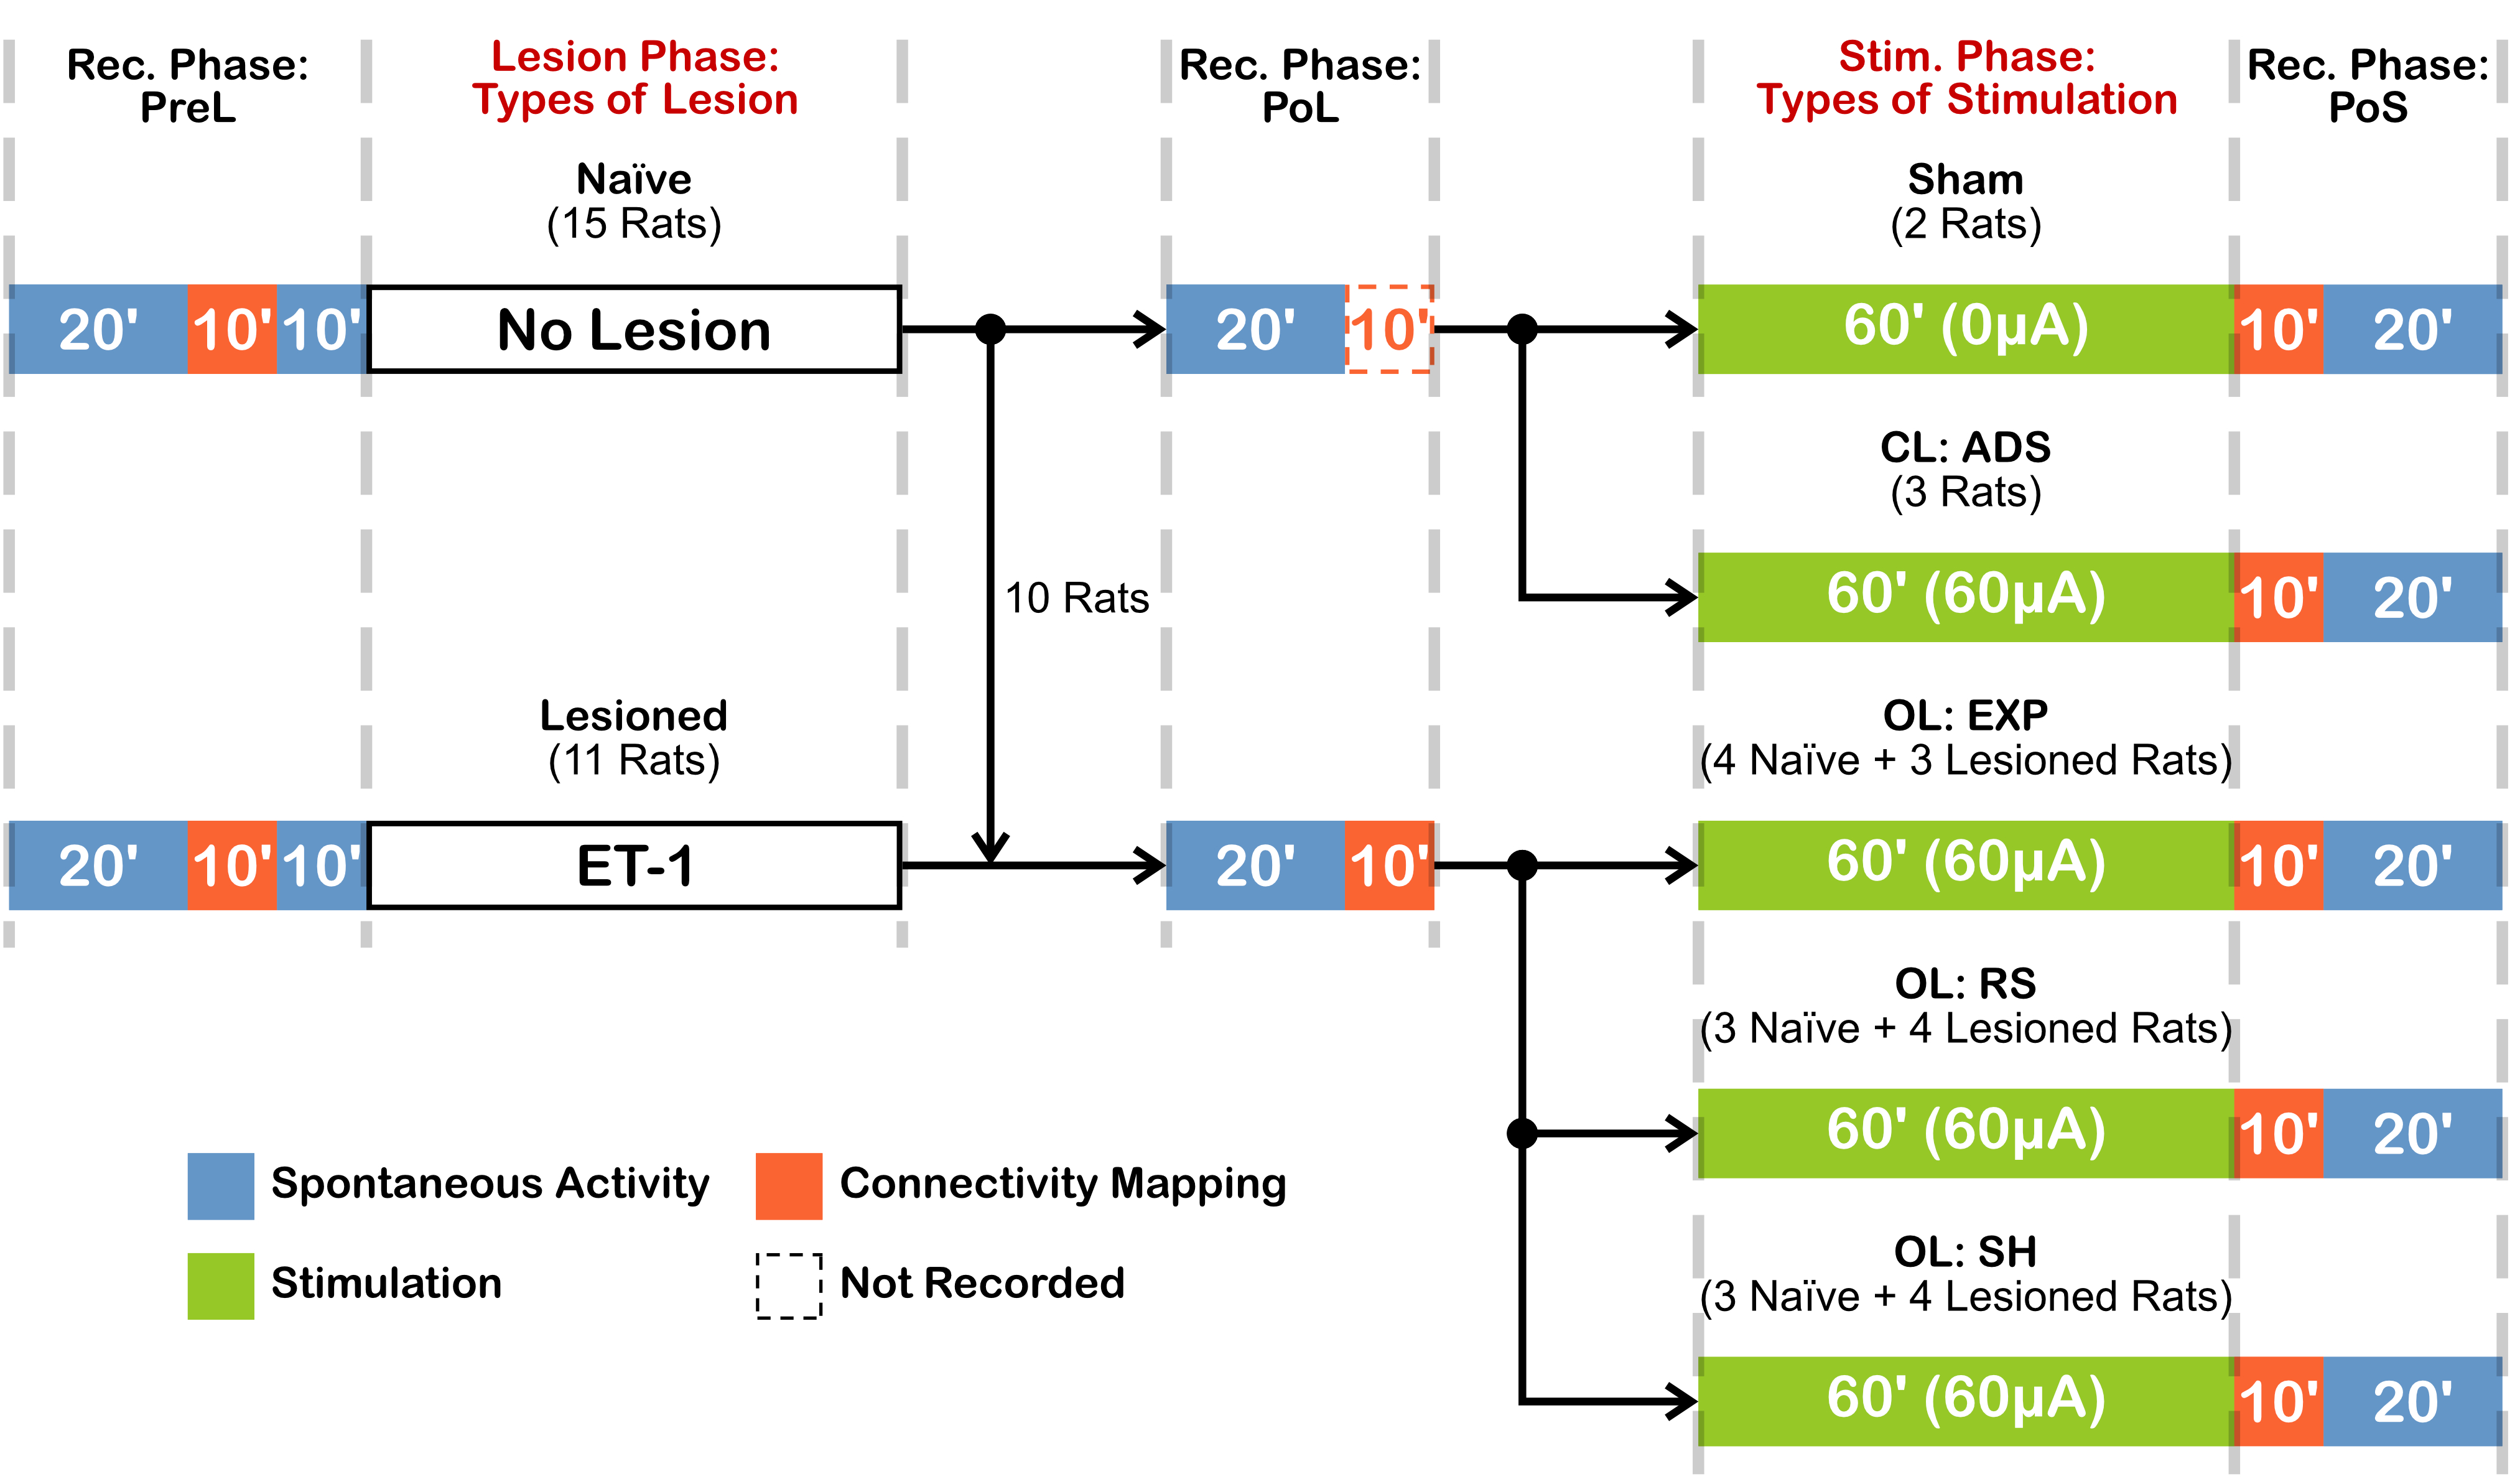
\includegraphics[width=\linewidth]{Figure/Experimental Protocol/Experimental Protocol.jpg}
    \end{center}
    \caption{Experimental timeline. All the phases of the experiment are depicted in the image, including the distribution of rats among the various experimental groups. Twenty-six rats were initially divided into two groups (Naïve and Lesioned), and then further subdivided into five groups based on the type of stimulation they received (Sham, Closed Loop: Activity Dependent Stimulation (CL: ADS), Open Loop: Exponential (OL: EXP), Open Loop: Repeated (OL: RS), Open Loop: Shuffling (OL: SH)) for a total of eight groups (Naïve-Sham, Naïve-CL:ADS, Naïve-OL: EXP, Naïve-OL: RS, Naïve-OL: SH, Lesioned-OL: EXP, Lesioned-OL: RS, Lesioned-OL: SH). All groups underwent the same Pre-Lesion (PreL) and Post-Stimulation (PoS) phases, but only those subjected to an open loop stimulation protocol underwent connectivity mapping recording during the Post-Lesion (PoL) phase.}
    \label{fig:Experimental Protocol}
\end{figure}

Extracellular signals have been continuously sampled at a rate of 25 kHz using standard, commercially available neurophysiological hardware (Intan RHS, Intan technologies LLC) and for better efficiency in the data processing step, data were saved in blocks of 10-min recordings each.

In the Naïve groups, a ‘No Lesion’ period was considered, which lasted approximately 1 hour. In the groups that received the stimulation (i.e. Naïve-Open Loop, Lesion-Open Loop and Naïve-Closed Loop) 1 hour of stimulation (e.g. Exponential, Repeated, Shuffling and Activity-Dependent Stimulation) was recorded, while in the Sham group was recorded one more spontaneous session (i.e. Sham). In all the experiments, the stimulation pulse was designed to be a single squared 60 µA biphasic, cathodal-leading pulse (200 µs positive, 200 µs negative), however in the Sham animals the pulse current was set to 0 µA.

Moreover, only in the groups that received an Open Loop stimulation, a Post-Lesion (PoL) Connectivity mapping recording was actually performed (Figure \ref{fig:Experimental Protocol}).

\subsubsection{Connectivity mapping phase}

An impedance analysis was performed and according to the lowest value (200-300 k$\Omega$), two single channels from S1 were selected to deliver the stimulations. Two different channels have been chosen to investigate whether the effects of stimulation could be location-dependent. In addition, two different frequencies were tested to explore potential variations in response speed. Specifically, the protocol for the connectivity mapping consisted of two recording steps to investigate evoked responses. (i) a stimulus was delivered every second for 1 minute (corresponding to a sample rate of 1 Hz), through two different channels, and a 30-sec of ‘no stimulation’ was recorded between the two channels. (ii) a stimulus was delivered every 5 seconds for a total of 30 times (resulting in a sample rate of 0.2 Hz), through two different channels, and a 30-sec of ‘no stimulation’ was recorded between the two channels.

\subsubsection{Stimulation phase}

An impedance analysis was performed on the S1 electrode and the single channel with the lowest impedance value (approximately 0.2 M$\Omega$) was chosen for delivering the stimulation.

For all the open loop stimulation methods, the following steps were followed: (i) During the first spontaneous activity recording, one of the sixteen channels in RFA was selected based on visual observation of spike amplitudes and signal to noise ratios; (ii) the timestamp was extracted; (iii) subsampling was done at a frequency of 1 kHz in order to load the stimulation vector onto Simulink; (iv) the stimulation pattern was created according to the chosen method, described above; (v) the stimulation was controlled using a model loaded onto Simulink, which was delivered through a breakout box connected to the INTAN RHS Stim/Recording System (intantech).

For the closed loop stimulation method, the first step followed was the same as the open loop methods, while the second step involved setting a channel-specific threshold in the Intan software, to act as the trigger for activity-dependent stimulation (ADS).

\subsection{Stimulation paradigms}

All the animals of the Lesion group and 10 Naïve rats were randomly assigned to one of the four stimulation groups (see Figure \ref{fig:Experimental Protocol}):
\begin{itemize}
    \item \textbf{OL: Exponential Stimulation:} the mean firing rate of the extracted time stamps from the first 20-min of the healthy spontaneous activity recorded before the lesion was used to design a new spike sequence according to a pre-defined/mathematical distribution, e.g., exponential distribution (Mathworks); 
    \item \textbf{OL: Repeated Stimulation:} the first 10-min of the healthy spontaneous activity recorded before the lesion (i.e., PreL) on a selected channel in RFA were looped six times to deliver a stimulation pattern lasting an hour \cite{Zullo2012};
    \item \textbf{OL: Shuffling Stimulation:} a new spike sequence of the duration of interest was generated according to a data-driven ISI, based on data acquired from a reference network;
    \item \textbf{CL: Activity-Dependent Stimulation:} a single stimulation pulse was delivered to a selected channel on the S1 probe each time the pre-configured threshold was crossed. To prohibit feedback from stimulus-evoked RFA spikes and stimulus artifacts from triggering stimulation, a blanking period (28 ms) followed each stimulus limiting the maximum stimulation rate to roughly 35 Hz.
\end{itemize}

\subsection{Data and Statistical Analyses}

\subsubsection{Preprocessing}

All the preprocessing of the in-vivo recordings was performed in MATLAB (The MathWorks, Natick, MA, USA). The ePhys data underwent preprocessing through a custom MATLAB pipeline. Briefly, data was formatted into a MATLAB-readable structure and organized on a per-channel basis. Subsequently, a 4th order elliptic bandpass filter (300-3000 Hz) was applied to eliminate low-frequency components in the signal. A power-based spike detection algorithm known as Stationary Wavelet-based Teager Energy Operator (SWTTEO) \cite{Lieb2017} was employed to identify spikes from the filtered data. The SWTTEO involved two levels of Stationary Wavelet Transform (SWT) followed by the use of the Teager Energy Operator (TEO). The TEO outputs were smoothed, summed, and their combination was thresholded. Multiunits were later sorted using a mixture of skew-t distributions on PCA-extracted features, following the approach outlined in \cite{Toosi2021}. Peaks that clearly corresponded to noise were excluded at this stage by assignment to a “noise” or “non-neural” source cluster.

\subsubsection{Post-Stimulus Time Histogram (PSTH)}

The evoked activity was assessed by computing the post-stimulus time histogram (PSTH) using an adapted version of a custom software package (SPYCODE) (Bologna et al. [2010]). A time window of 800 ms, a bin size of 4 ms and a blanking period of 0.4 ms were chosen. Two separate PSTHs and the corresponding areas under the PSTH curve were calculated for each electrode (multi-unit activity). This separation aimed to distinguish the PSTH generated by the first stimulation channel from the one generated by the second channel (e.g., the first PSTH and area under the PSTH curve considered the first 30 stimuli).

\subsubsection{Statistical Analysis}

The statistical analysis was performed in MATLAB as well. For each rat two mean values were considered: one for the PSTH areas obtained with a stimulation frequency of 1Hz and one for the PSTH areas obtained with 0.2Hz. To identify differences in the PSTH areas between all the phases of the experimental protocol (PreL, PoL and PoS) a one-way ANOVA test was performed. P-values were considered significant for $p<0.05$.

\section{Results}

To analyze how the lesion and the subsequent stimulation phase affect the networks, stimulations at two different frequencies (1 Hz and 0.2 Hz) were delivered to map the recorded areas. The PSTH analysis of the connectivity mapping stimulations was used to assess the intra- and inter-area evoked responses.
In Figure \ref{fig:RasterPSTH}, the activity elicited by the 0.2Hz stimulus is illustrated. This activity was recorded in one of the channels from both the RFA and the S1 areas of a representative animal that received shuffled stimulation after the lesion. Additionally, Figure \ref{fig:PSTH} depicts a representative Post-Stimulus Time Histogram (PSTH) of the evoked response after the 0.2Hz stimulus in the same animal.

\begin{figure}[htp]
    \begin{center}
    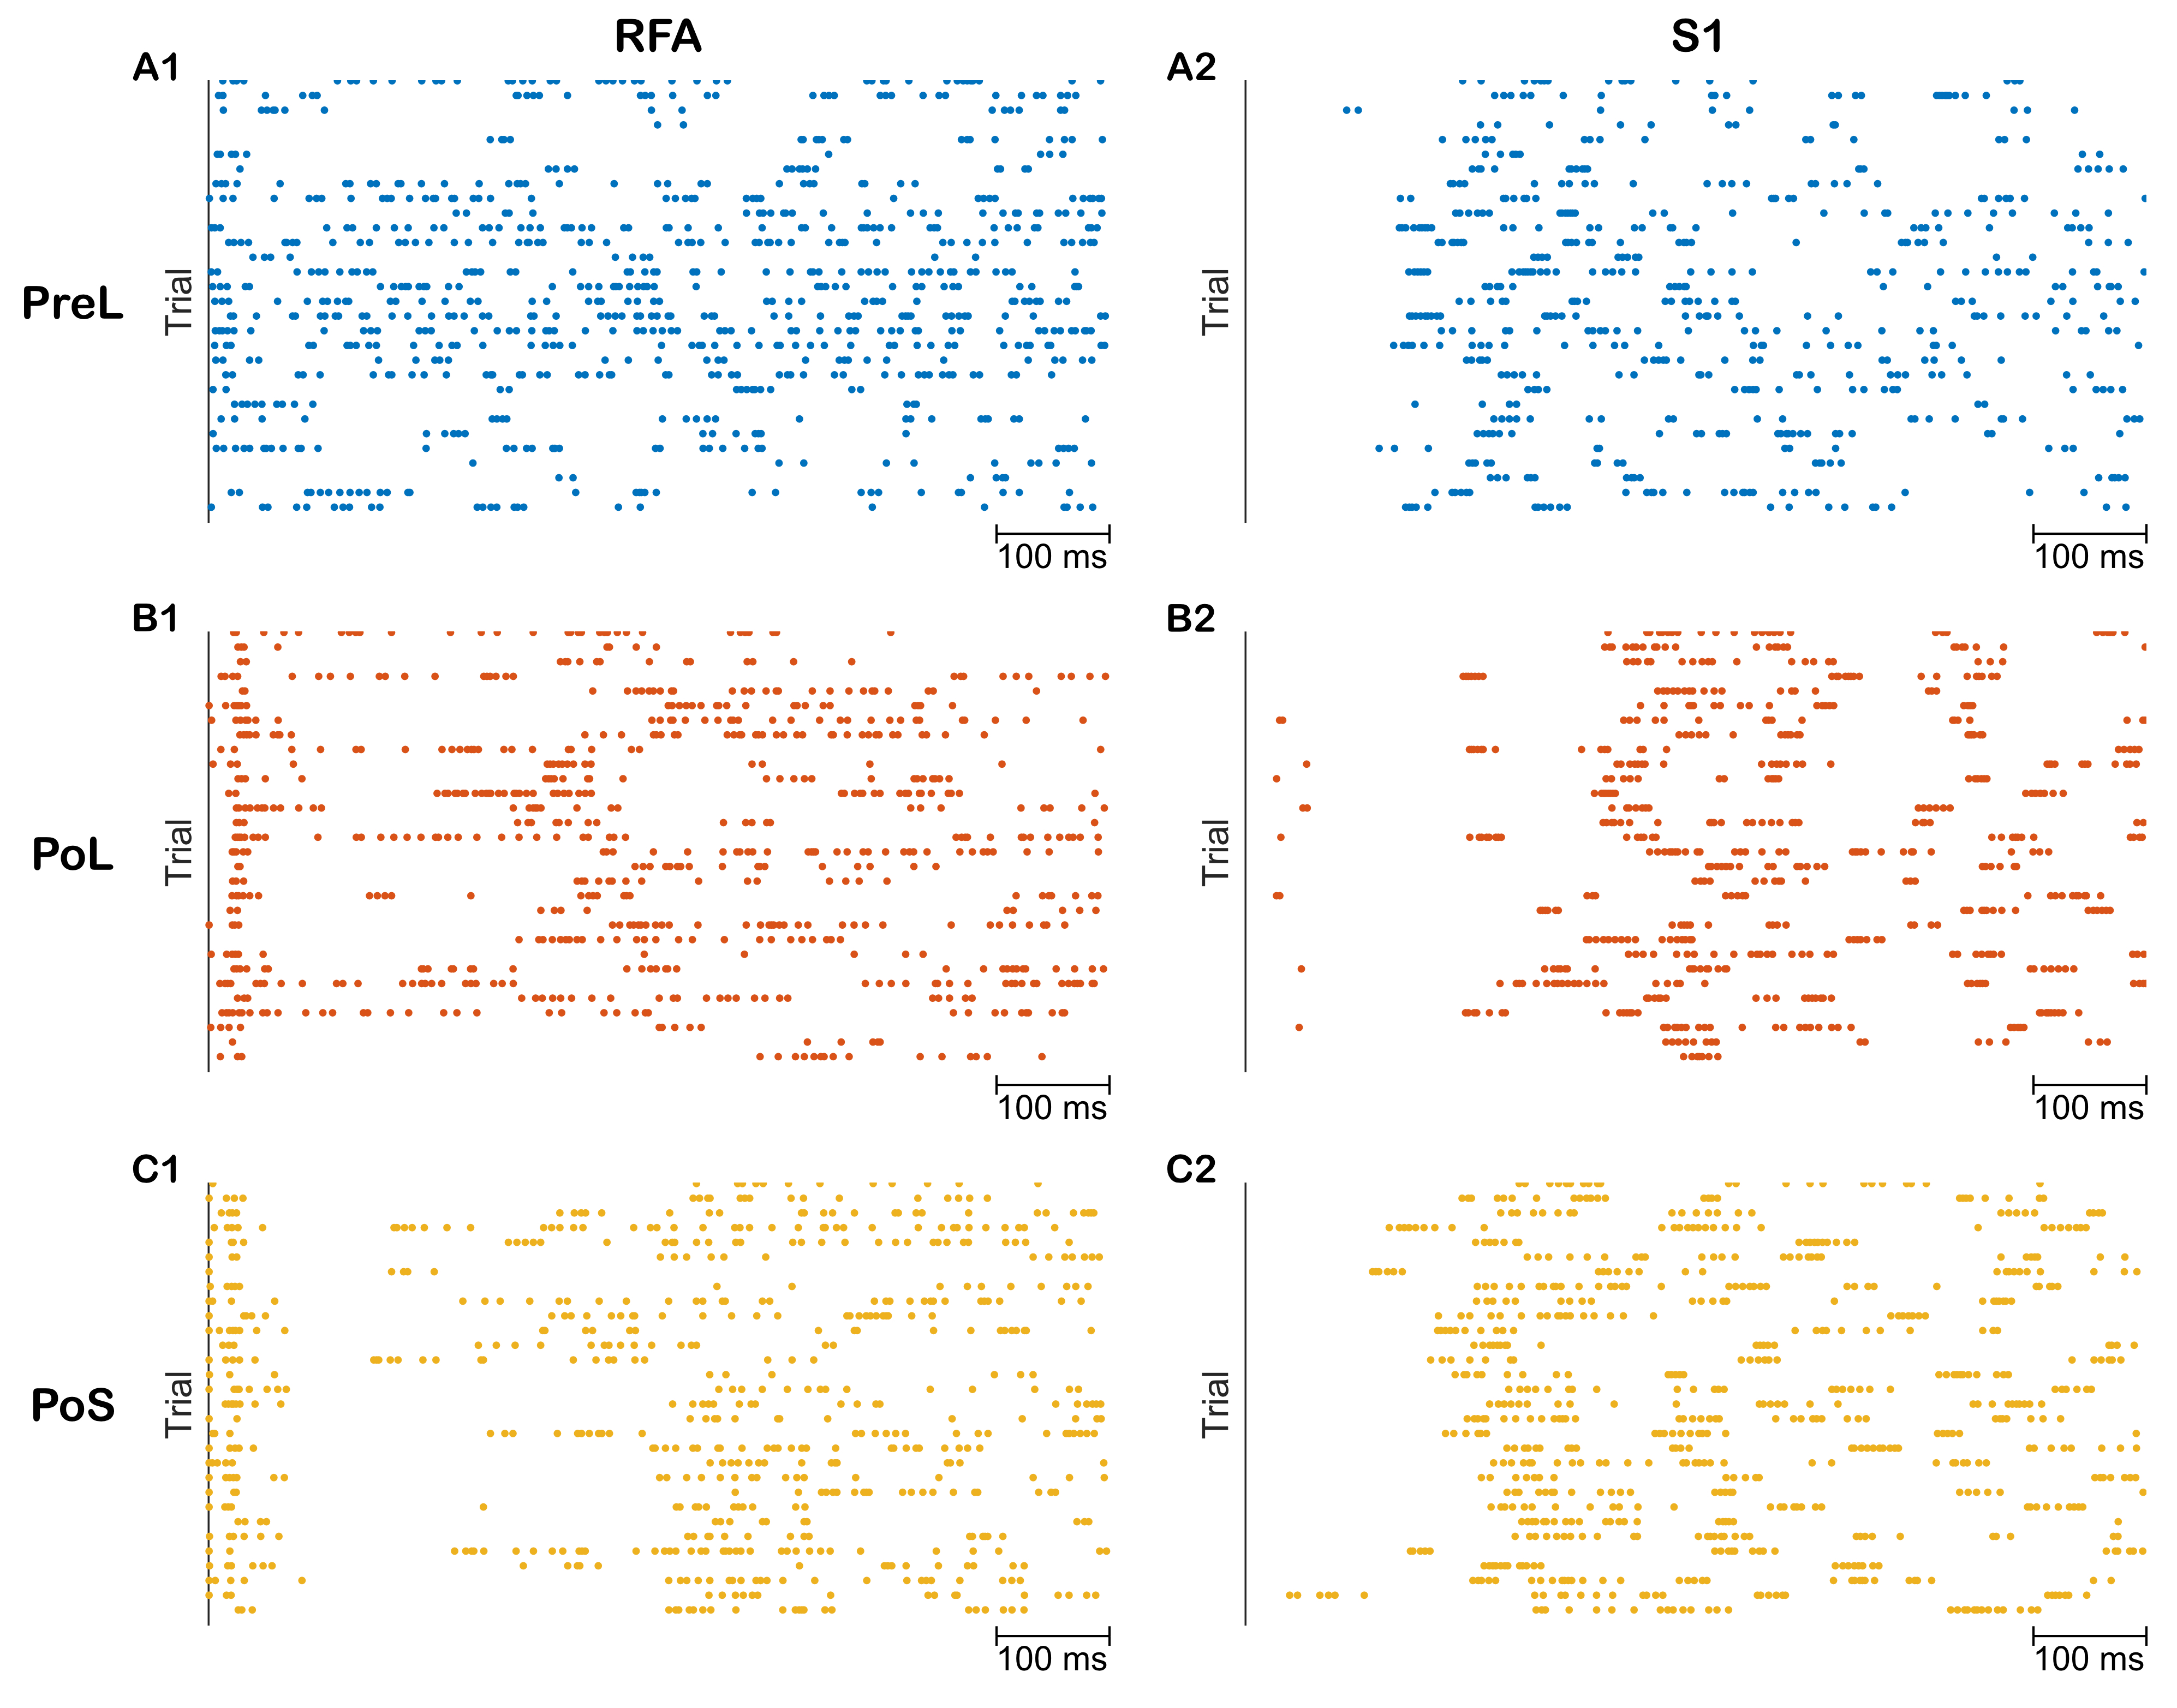
\includegraphics[width=\linewidth]{Figure/rasterplot PSTH/RasterPSTH.jpg}
    \end{center}
    \caption{Firing Activity Evoked by the Connectivity Mapping Stimulations. (A) 800-ms raster plots depict the recorded activity in the RFA (left) and S1 (right) areas after the connectivity mapping stimulation before the lesion (PreL, blue). (B) 800-ms raster plots illustrate the recorded activity in the RFA and S1 areas after the connectivity mapping stimulation following the lesion (PoL, orange). (C) 800-ms raster plots show the recorded activity in the RFA and S1 areas after the connectivity mapping stimulation following the delivery of personalized stimulation (PoS, yellow).}
    \label{fig:RasterPSTH}
\end{figure}

\begin{figure}[htp]
    \begin{center}
    \includegraphics[width=\linewidth]{Figure/PSTH/PSTH.jpg}
    \end{center}
\end{figure}
\begin{figure}[p!]
    \caption{(figure in the previous page) PSTH graphs. Each graph represent the PSTH of a single channel before (blue) and after (orange) the lesion, and after the stimulation (yellow). On the top, the PSTHs in the stimulation area (i.e., S1), and the red square highlights the stimulation channel. On the bottom, the evoked responses in the recording area (i.e., RFA). The channels are spatially ordered as in the arrays. On the x-axis there is the time in seconds, on the y-axis there is the firing rate in spikes per seconds.}
    \label{fig:PSTH}
\end{figure}
\clearpage

\subsection{The effect of the ischemic lesion on the evoked responses}

This analysis was also employed to investigate whether the lesion could be localized and impact some regions more than others. In particular, the area under the PSTH of the Lesioned and Naïve animals that recieved both PreL and PoL connectivity mapping recordings were considered to obtain an overall understanding about the efficacy of the lesion. In Figures \ref{fig:Lesion Effect 0.2Hz} and \ref{fig:Lesion Effect 1Hz}, a more significant decrease in the PSTH area can be appreciated in both areas of the rats that received a lesion compared to those in the Naïve group. In particular, considering the slope of the regression lines, it’s possible to emphasize and evaluate the negative impact of the lesion on the evoked responses. The Naïve group, indeed, exhibits a higher slope than the group that actually underwent the lesion.

\begin{figure}[ht!]
    \begin{center}
    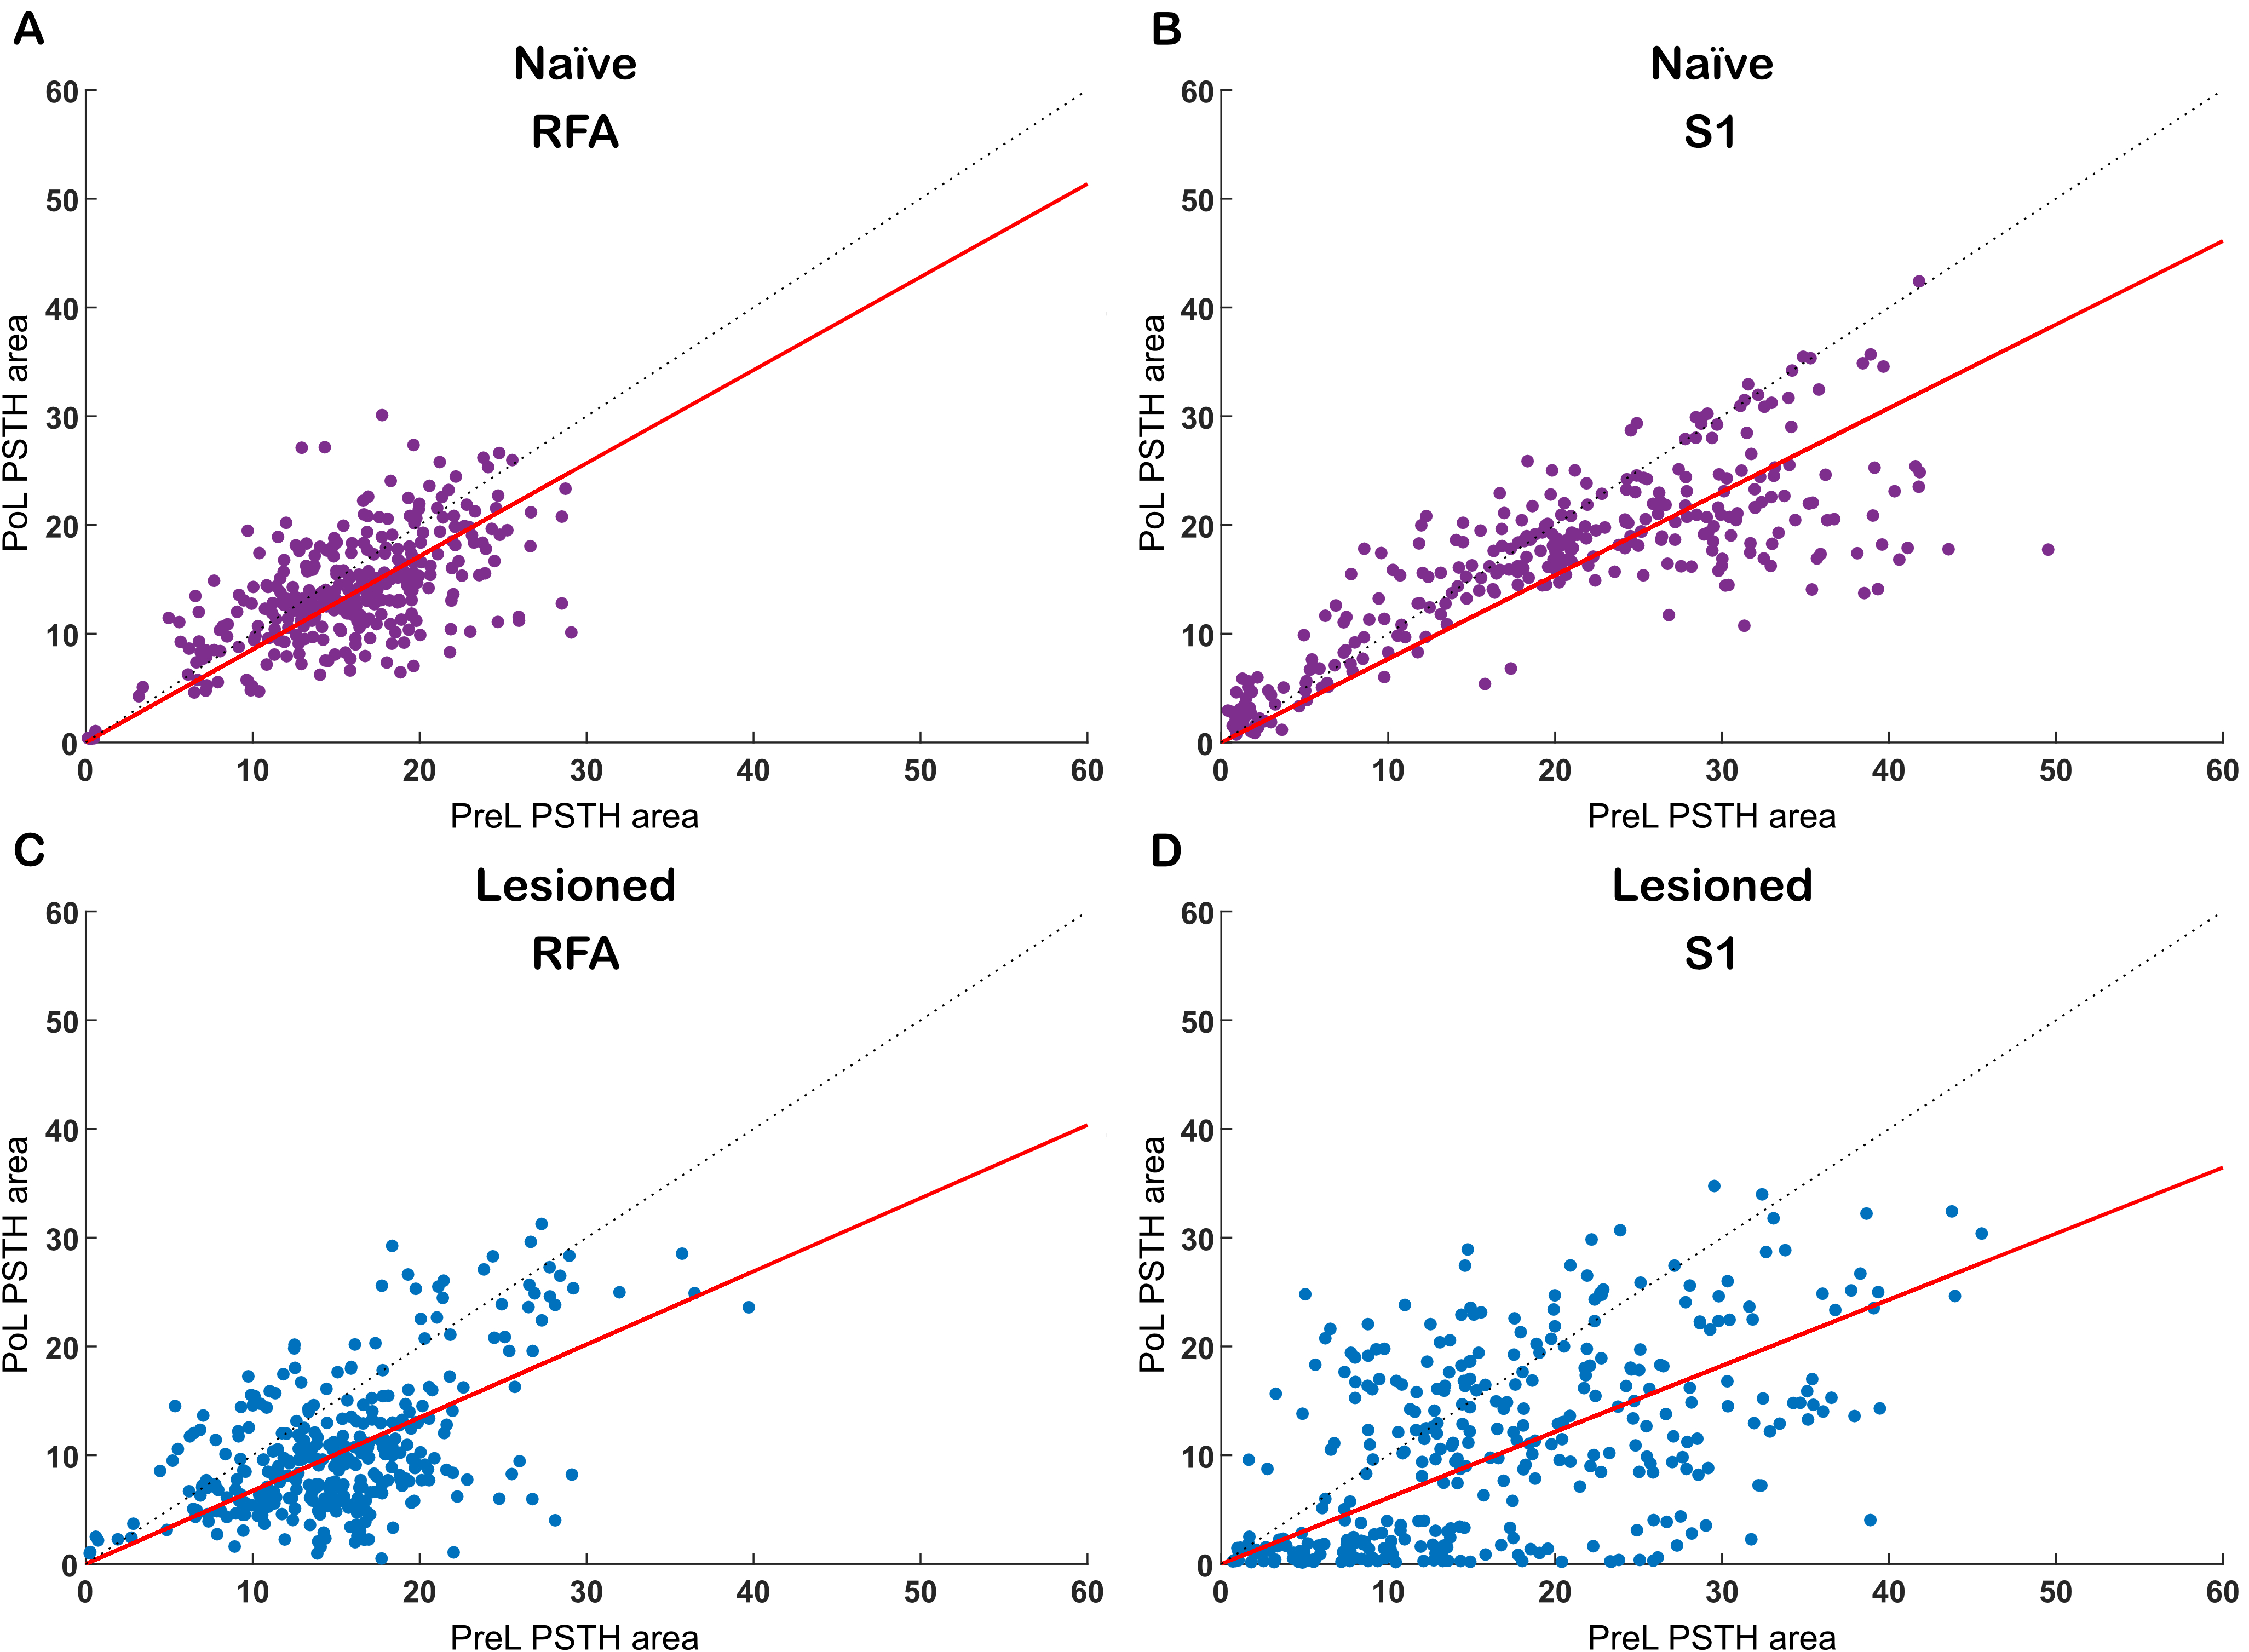
\includegraphics[width=\linewidth]{Figure/Lesion Effect/Lesion Effect 0.2Hz.jpg}
    \end{center}
    \caption{Pre-Lesion and Post-Lesion PSTH area for the 0.2Hz stimulation rate. Left: results in RFA. Right: results in S1. (A, B) On the top: scatterplot of the PSTH area in the Naïve group. (C, D) On the bottom: scatterplot of the PSTH area in the Lesioned group. On the x-axis is showed the Pre-Lesion (PreL) PSTH area and on the y-axis the Post-Lesion (PoL) PSTH area. Each dot represent a channel. The dotted line represents the bisector with a slope of 1. The red line represent the regression line of the dots that pass through the center of axes (slopes: A: 0.86, B: 0.77, C: 0.67, D: 0.61).}
    \label{fig:Lesion Effect 0.2Hz}
\end{figure}

\begin{figure}[ht!]
    \begin{center}
    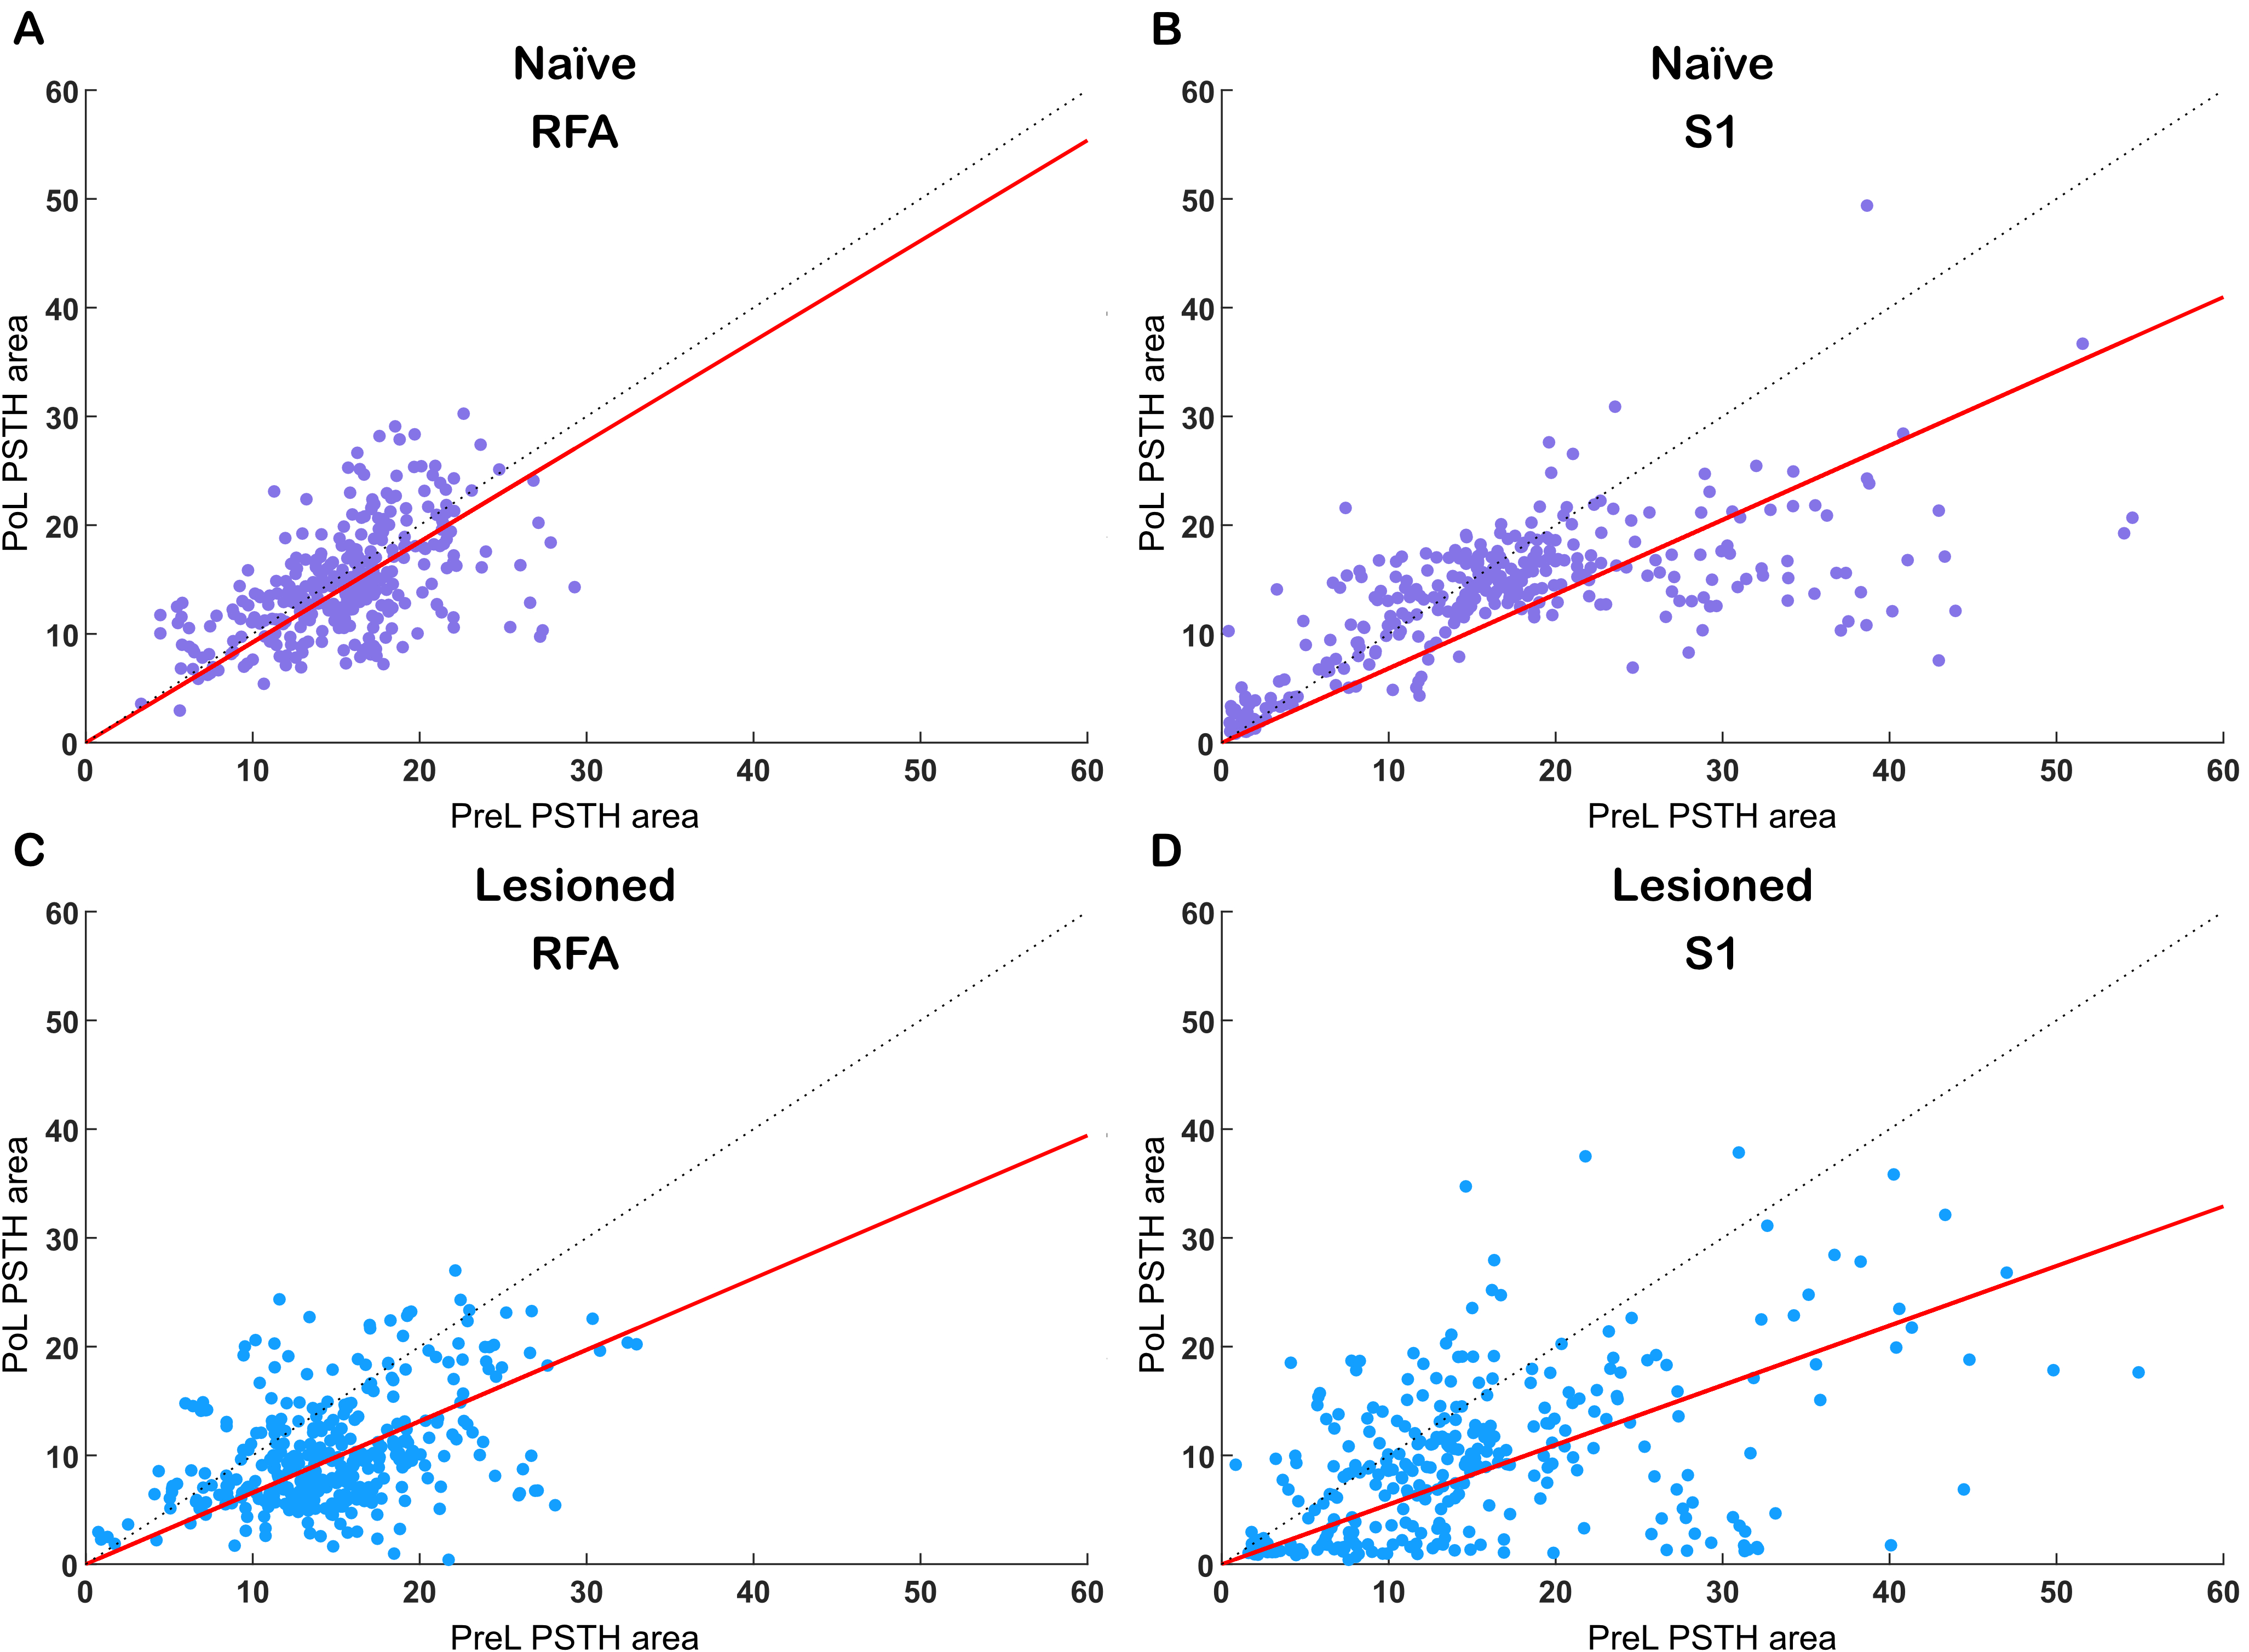
\includegraphics[width=\linewidth]{Figure/Lesion Effect/Lesion Effect 1Hz.jpg}
    \end{center}
    \caption{Pre-Lesion and Post-Lesion PSTH area for the 1Hz stimulation rate. Left: results in RFA. Right: results in S1. (A, B) On the top: scatterplot of the PSTH area in the Naïve group. (C, D) On the bottom: scatterplot of the PSTH area in the Lesioned group. On the x-axis is showed the Pre-Lesion (PreL) PSTH area and on the y-axis the Post-Lesion (PoL) PSTH area. Each dot represent a channel. The dotted line represents the bisector with a slope of 1. The red line represent the regression line of the dots that pass through the center of axes (slopes: A: 0.92, B: 0.68, C: 0.66, D: 0.55).}
    \label{fig:Lesion Effect 1Hz}
\end{figure}

This behavior can also be observed in Figure \ref{fig:ratio PoL-PreL PSTH area 0.2Hz} and \ref{fig:ratio PoL-PreL PSTH area 1Hz} A, B, and is confirmed by statistical analysis. Indeed, the lesion significantly decreases the PSTH area from the PreL to PoL phase in the RFA area when the connectivity mapping stimuli are delivered with a frequency of 1Hz ($p<0.05$, one-way ANOVA). With the same frequency, the null hypothesis is not rejected in S1 ($p=0.149$), as well as when the connectivity mapping stimuli frequency is 0.2Hz (RFA: $p=0.062$; S1: $p=0.434$). Notably, the number of channels exhibiting activity during the PoL phase lower than the mean activity of the PreL phase is greater than 50\% (Figure \ref{fig:ratio PoL-PreL PSTH area 0.2Hz} and \ref{fig:ratio PoL-PreL PSTH area 1Hz} C, D).

\begin{figure}[ht!]
    \begin{center}
    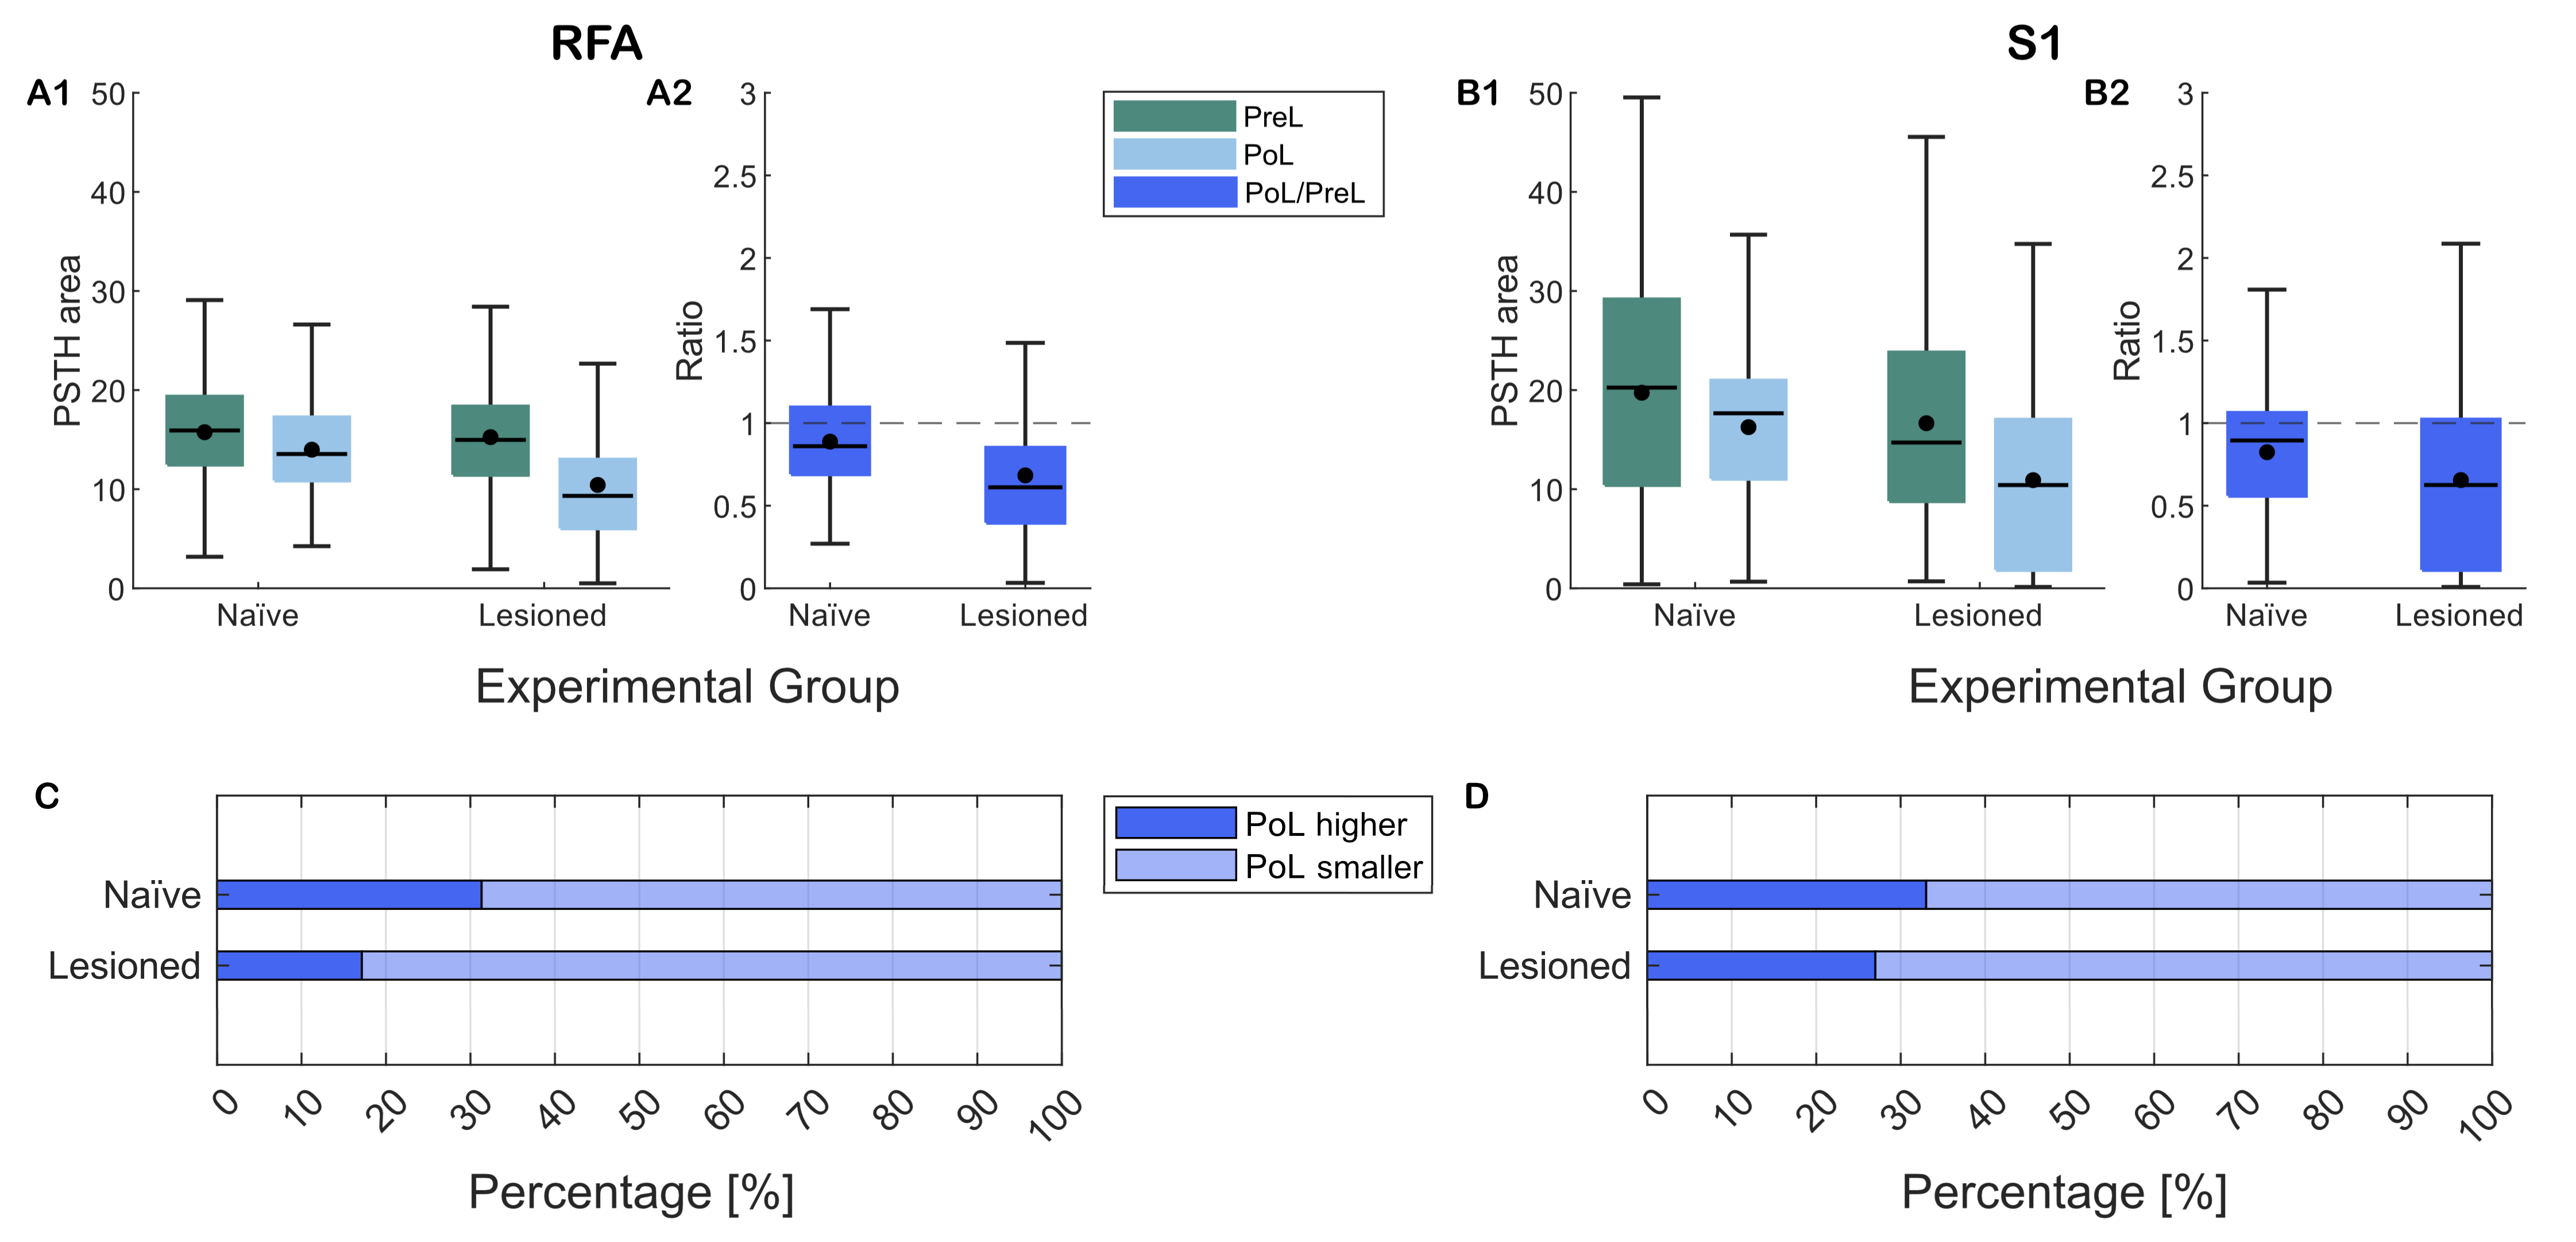
\includegraphics[width=\linewidth]{Figure/Ratio PSTH area separate/ratio PoL-PreL PSTH area 0.2Hz.jpg}
    \end{center}
    \caption{Effect of lesion on the evoked response (Connectivity Mapping stimulation 0.2Hz). (A) Box plot of the PSTH area of RFA for the entire dataset of Naïve and Lesioned rats stimulated with an OL (EXP, RS, SH) paradigm. (B) Box plot of the PSTH area of S1 for the entire dataset of Naïve and Lesioned rats stimulated with an OL (EXP, RS, SH) paradigm. (A2, B2) Box plot of the ratio between the PSTH area of the PoL phase with the mean PSTH area of the PreL phase. For each box plot (A, B), the central black line indicates the median, the central black dot indicates the mean and the box limits indicate the 25th and 75th percentiles. The whiskers show the Q1-1.5*IQR and Q3+1.5*IQR, where Q1 and Q3 are the first and third quartiles, while the IQR is the interquartile range (the distance between Q1 and Q3). (C, D) Bar plot of the percentage of channels of RFA and S1 that has an PSTH area in the PoL phase greater than the mean PSTH area in the PreL phase, for the entire dataset of Naïve and Lesioned rats stimulated with an OL (EXP, RS, SH) paradigm.}
    \label{fig:ratio PoL-PreL PSTH area 0.2Hz}
\end{figure}

\begin{figure}[ht!]
    \begin{center}
    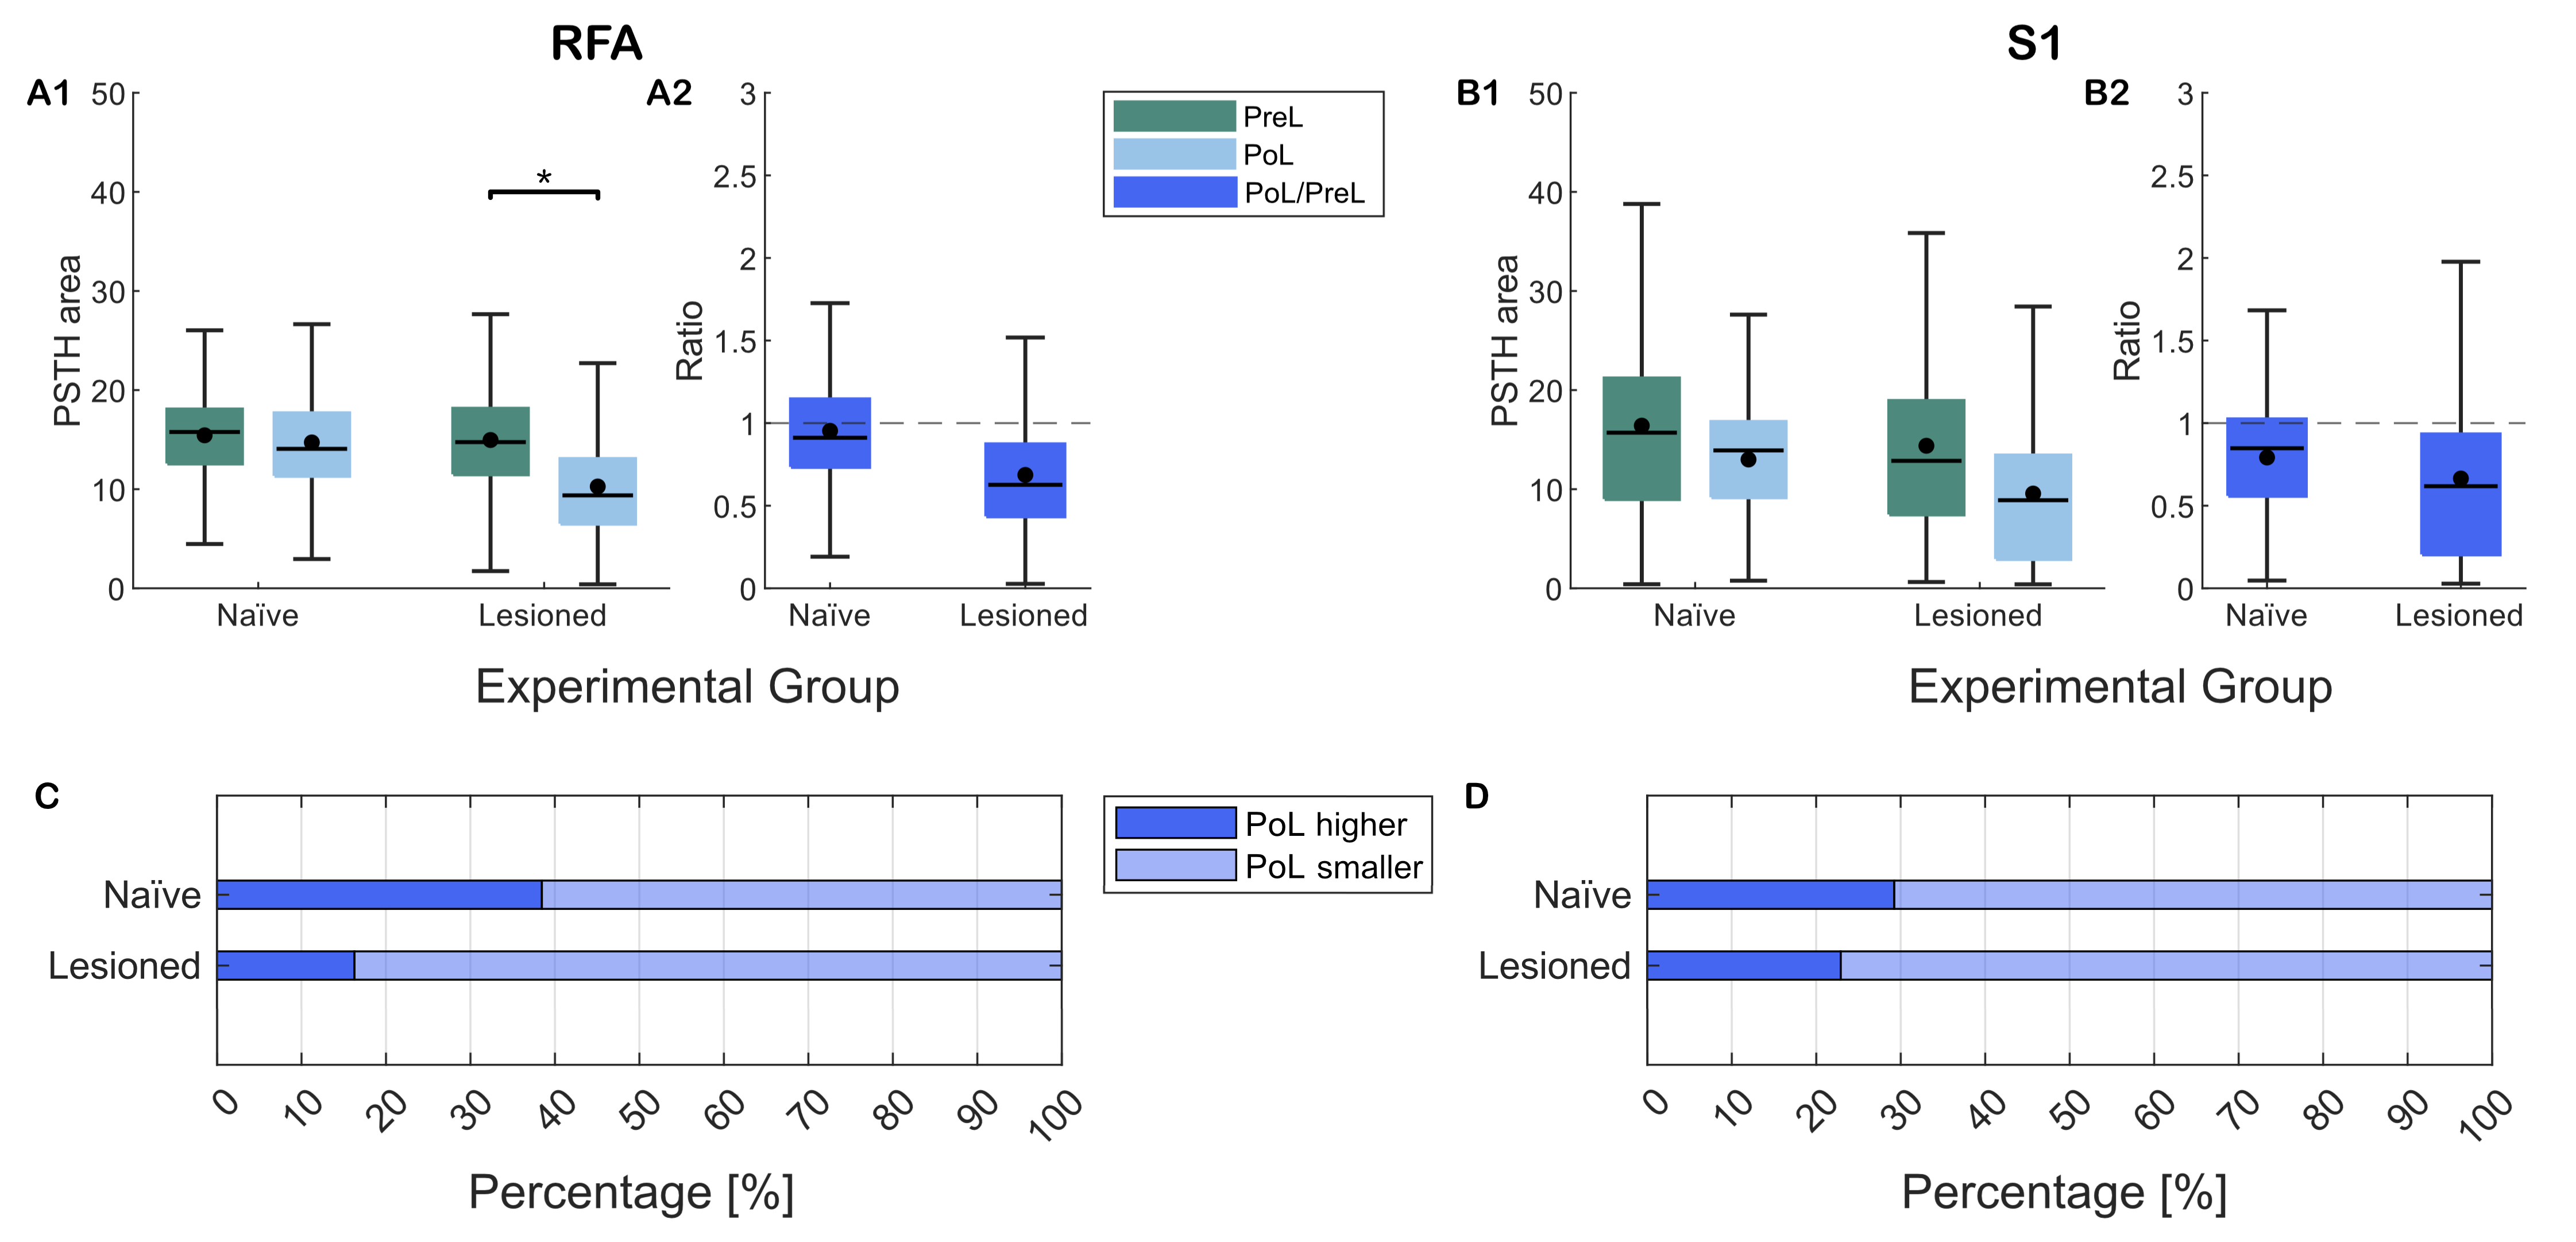
\includegraphics[width=0.90\linewidth]{Figure/Ratio PSTH area separate/ratio PoL-PreL PSTH area 1Hz.jpg}
    \end{center}
    \caption{Effect of lesion on the evoked response (Connectivity Mapping stimulation 1Hz). (A) Box plot of the PSTH area of RFA for the entire dataset of Naïve and Lesioned rats stimulated with an OL (EXP, RS, SH) paradigm. (B) Box plot of the PSTH area of S1 for the entire dataset of Naïve and Lesioned rats stimulated with an OL (EXP, RS, SH) paradigm. (A2, B2) Box plot of the ratio between the PSTH area of the PoL phase with the mean PSTH area of the PreL phase. For each box plot (A, B), the central black line indicates the median, the central black dot indicates the mean and the box limits indicate the 25th and 75th percentiles. The whiskers show the Q1-1.5*IQR and Q3+1.5*IQR, where Q1 and Q3 are the first and third quartiles, while the IQR is the interquartile range (the distance between Q1 and Q3). Solid line *: $p<0.05$, one-way ANOVA test. (C, D) Bar plot of the percentage of channels of RFA and S1 that has an PSTH area in the PoL phase greater than the mean PSTH area in the PreL phase, for the entire dataset of Naïve and Lesioned rats stimulated with an OL (EXP, RS, SH) paradigm.}
    \label{fig:ratio PoL-PreL PSTH area 1Hz}
\end{figure}

\clearpage
\subsection{The effect of the experimental procedure on the evoked responses}

The aim of this analysis was to assess the impact of the experimental procedures on evoked activity and their ability to restore the Pre-Lesion activity level.

The previous analysis revealed a global decrease in activity in both the Naïve and Lesioned groups during the Post-Lesion (PoL) phase.

Figure \ref{fig:PSTH area PreL-PoS 0.2Hz} and Figure \ref{fig:PSTH area PreL-PoS 1Hz} highlights that, even after the stimulation phase, all experimental groups (both Naïve and Lesioned) still exhibit decreased activity in both areas (RFA and S1), except for the group that received Closed Loop, Activity-Dependent Stimulation (CL: ADS), showing increased activity in the RFA area.

Focusing on the Naïve group, it is evident that the CL: ADS paradigm effectively increases the connectivity between the two areas, leveraging plasticity. In contrast, the other paradigms do not noticeably impact this interplay, as they fail to bring the activity levels back to the Pre-Lesion state.

\begin{figure}[htp]
    \begin{center}
    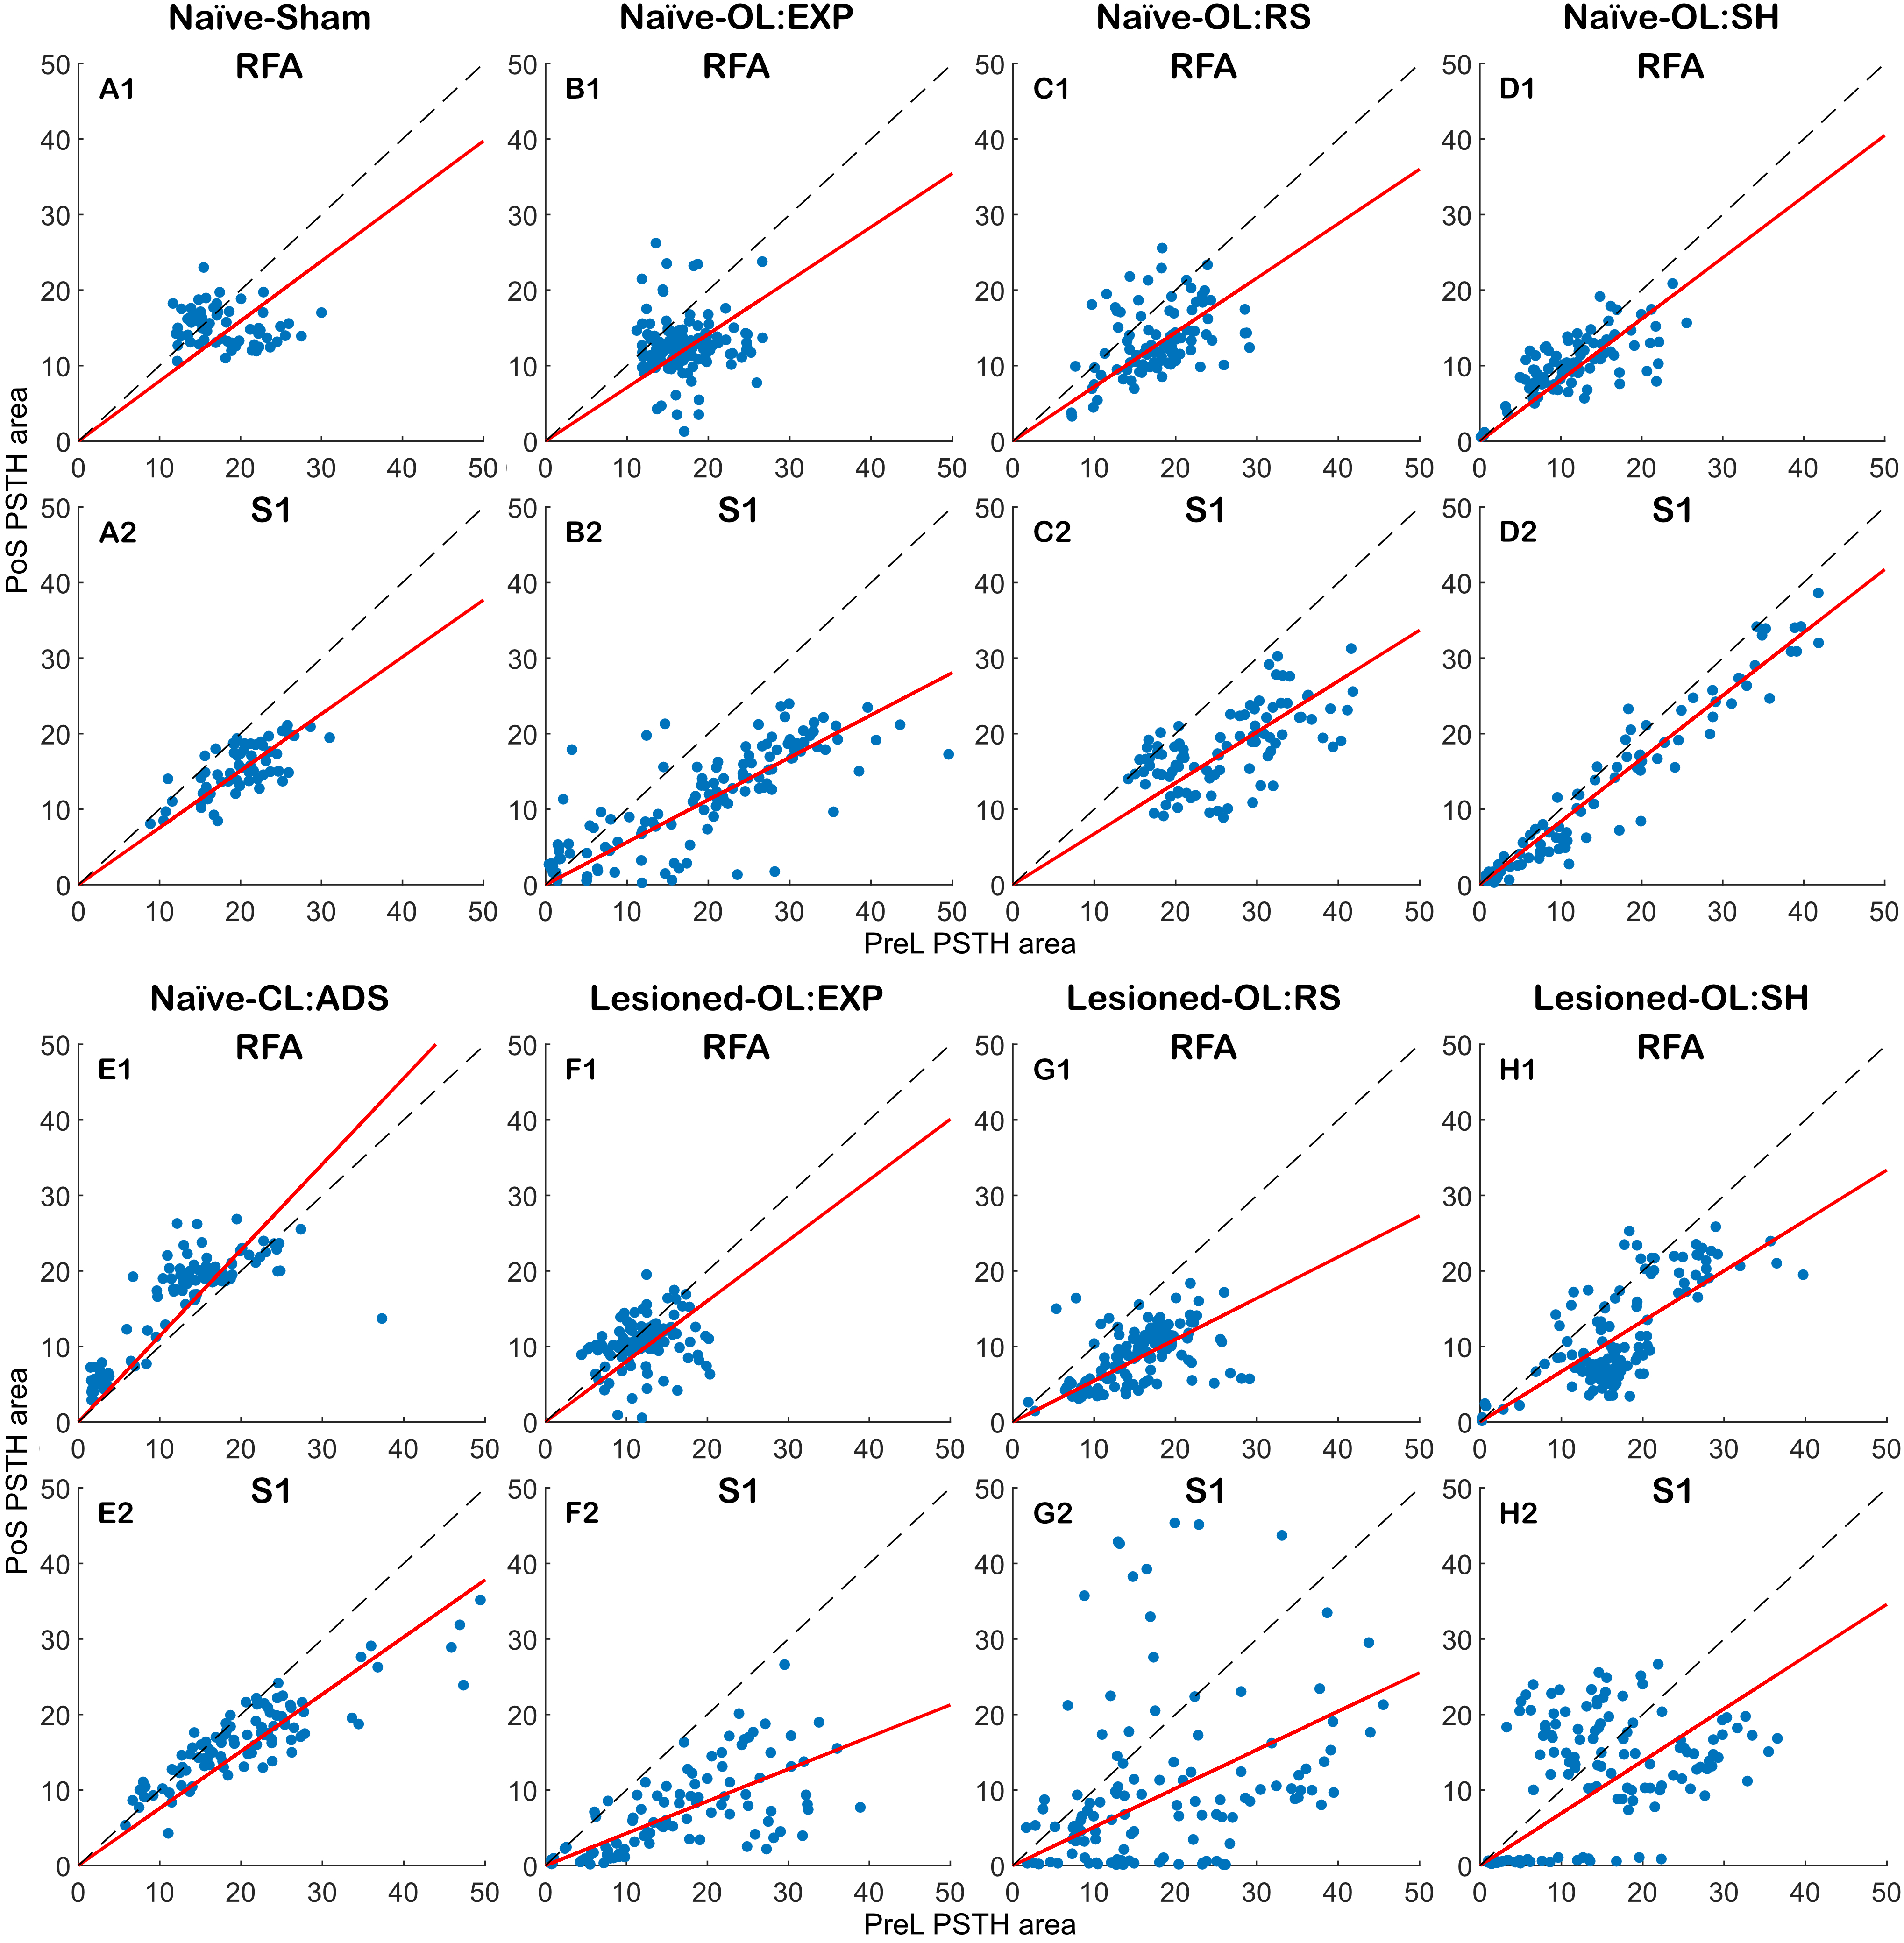
\includegraphics[width=\linewidth]{Figure/PSTH area PreL-PoS/PSTH area PreL-PoS 0.2Hz.jpg}
    \end{center}
\end{figure}
\begin{figure}[p!]
    \caption{(figure in the previous page) Pre-Lesion and Post-Stimulation PSTH area for the 0.2Hz stimulation rate. On the x-axis is showed the Pre- Lesion (PreL) PSTH area and on the y-axis the Post-Lesion (PoL) PSTH area. Each dot represent a channel. The dotted line represents the bisector with a slope of 1. The red line represent the regression line of the dots that pass through the center of axes (slopes: A1, A2: 0.79, 0.75; B1, B2: 0.71, 0.56; C1, C2: 0.72, 0.67; D1, D2: 0.81, 0.83; E1, E2: 1.14, 0.76; F1, F2: 0.80, 0.43; G1, G2: 0.55, 0.51; H1, H2: 0.67, 0.69).}
    \label{fig:PSTH area PreL-PoS 0.2Hz}
\end{figure}
\clearpage

\begin{figure}[htp]
    \begin{center}
    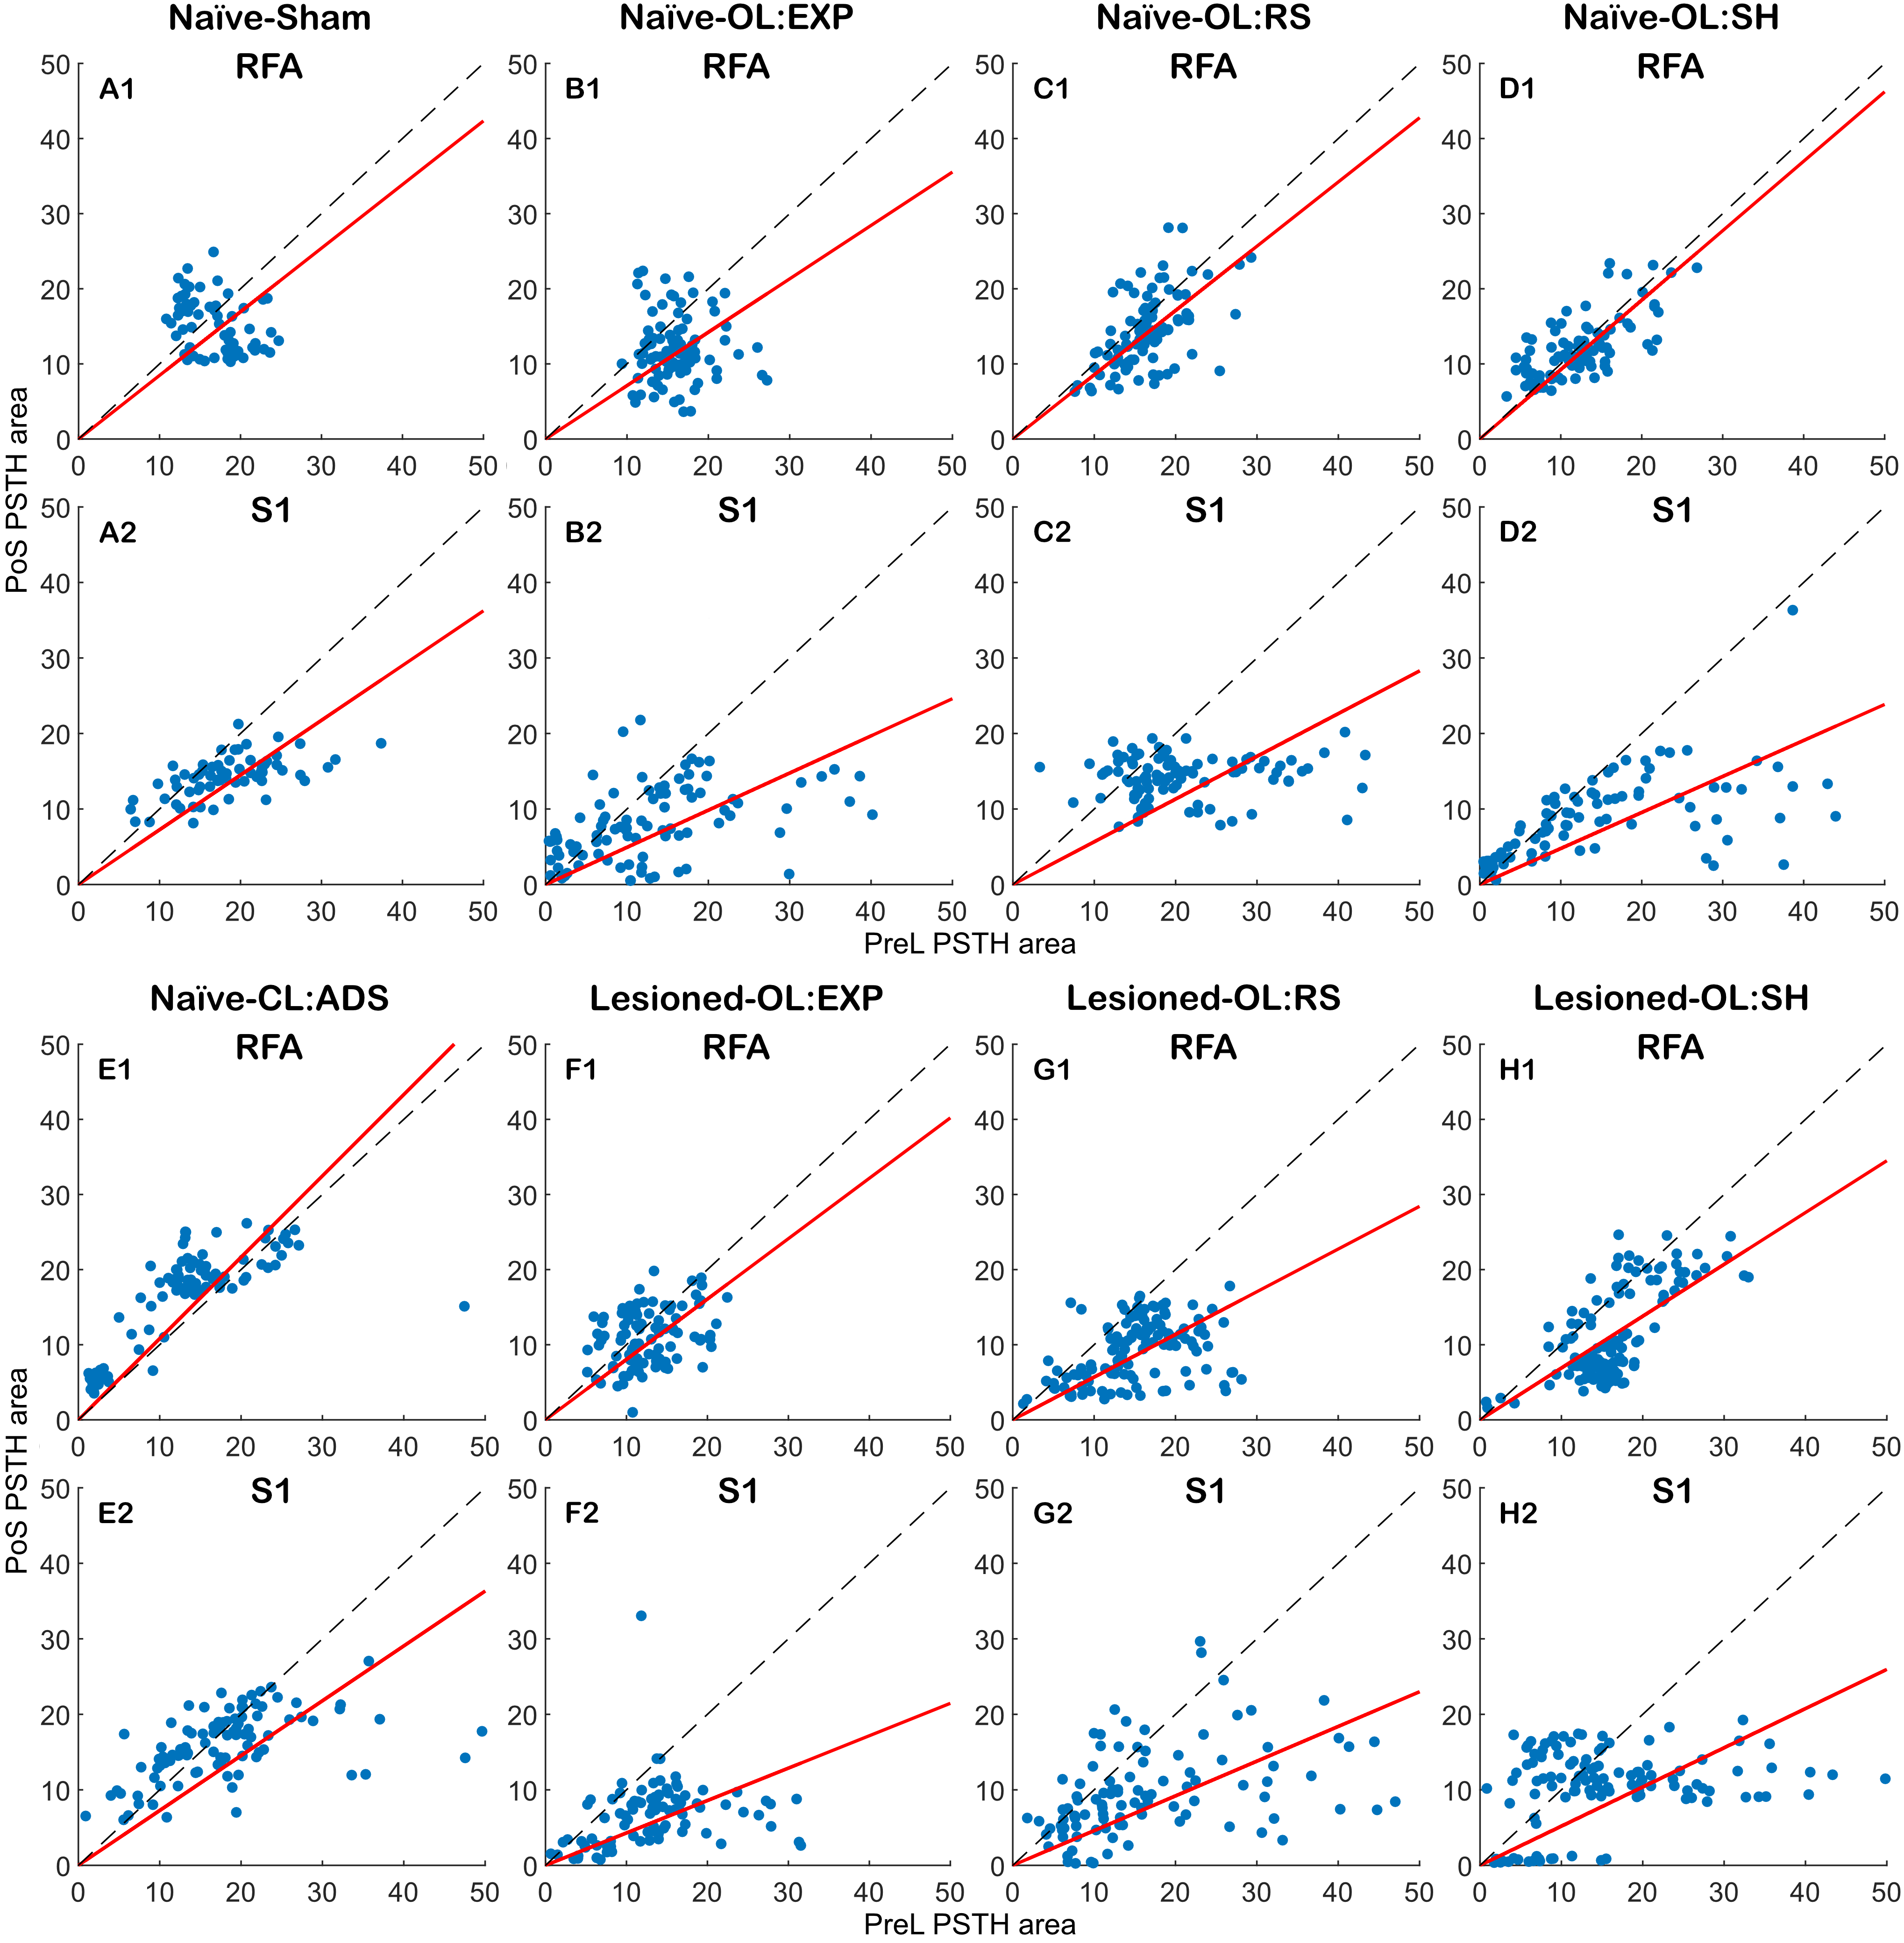
\includegraphics[width=\linewidth]{Figure/PSTH area PreL-PoS/PSTH area PreL-PoS 1Hz.jpg}
    \end{center}
\end{figure}
\begin{figure}[p!]
    \caption{(figure in the previous page) Pre-Lesion and Post-Stimulation PSTH area for the 1Hz stimulation rate. On the x-axis is showed the Pre- Lesion (PreL) PSTH area and on the y-axis the Post-Lesion (PoL) PSTH area. Each dot represent a channel. The dotted line represents the bisector with a slope of 1. The red line represent the regression line of the dots that pass through the center of axes (slopes: A1, A2: 0.85, 0.72; B1, B2: 0.71, 0.49; C1, C2: 0.86, 0.57; D1, D2: 0.92, 0.48; E1, E2: 1.08, 0.73; F1, F2: 0.80, 0.43; G1, G2: 0.57, 0.46; H1, H2: 0.69, 0.52).}
    \label{fig:PSTH area PreL-PoS 1Hz}
\end{figure}

\clearpage
\subsection{The effect of the Open Loop stimulations on the evoked responses}

In Figure \ref{fig:ratio all PSTH area 0.2Hz} and \ref{fig:ratio all PSTH area 1Hz}, it is depicted how the area under the PSTH keeps decreasing, even after the stimulation protocol, in the majority of the cases. However there are no significant differences between the PreL, PoL and PoS phases.

Analyzing the effect of the stimulation on the Naïve animals, it's evident that in all the cases this leads to a further decrease of the evoked response, in addition to the decrease yield by the lesion (Figure \ref{fig:ratio all PSTH area 0.2Hz} and \ref{fig:ratio all PSTH area 1Hz}). This behaviour is not always true in the lesioned animals, where the OL: SH paradigms leads to more channels with an higher evoked activity in S1 (Figure \ref{fig:ratio all PSTH area 0.2Hz} E, F, G, H) or RFA(Figure \ref{fig:ratio all PSTH area 1Hz} E, F, G, H) compared to the PreL phase.

\begin{figure}[htp]
    \begin{center}
    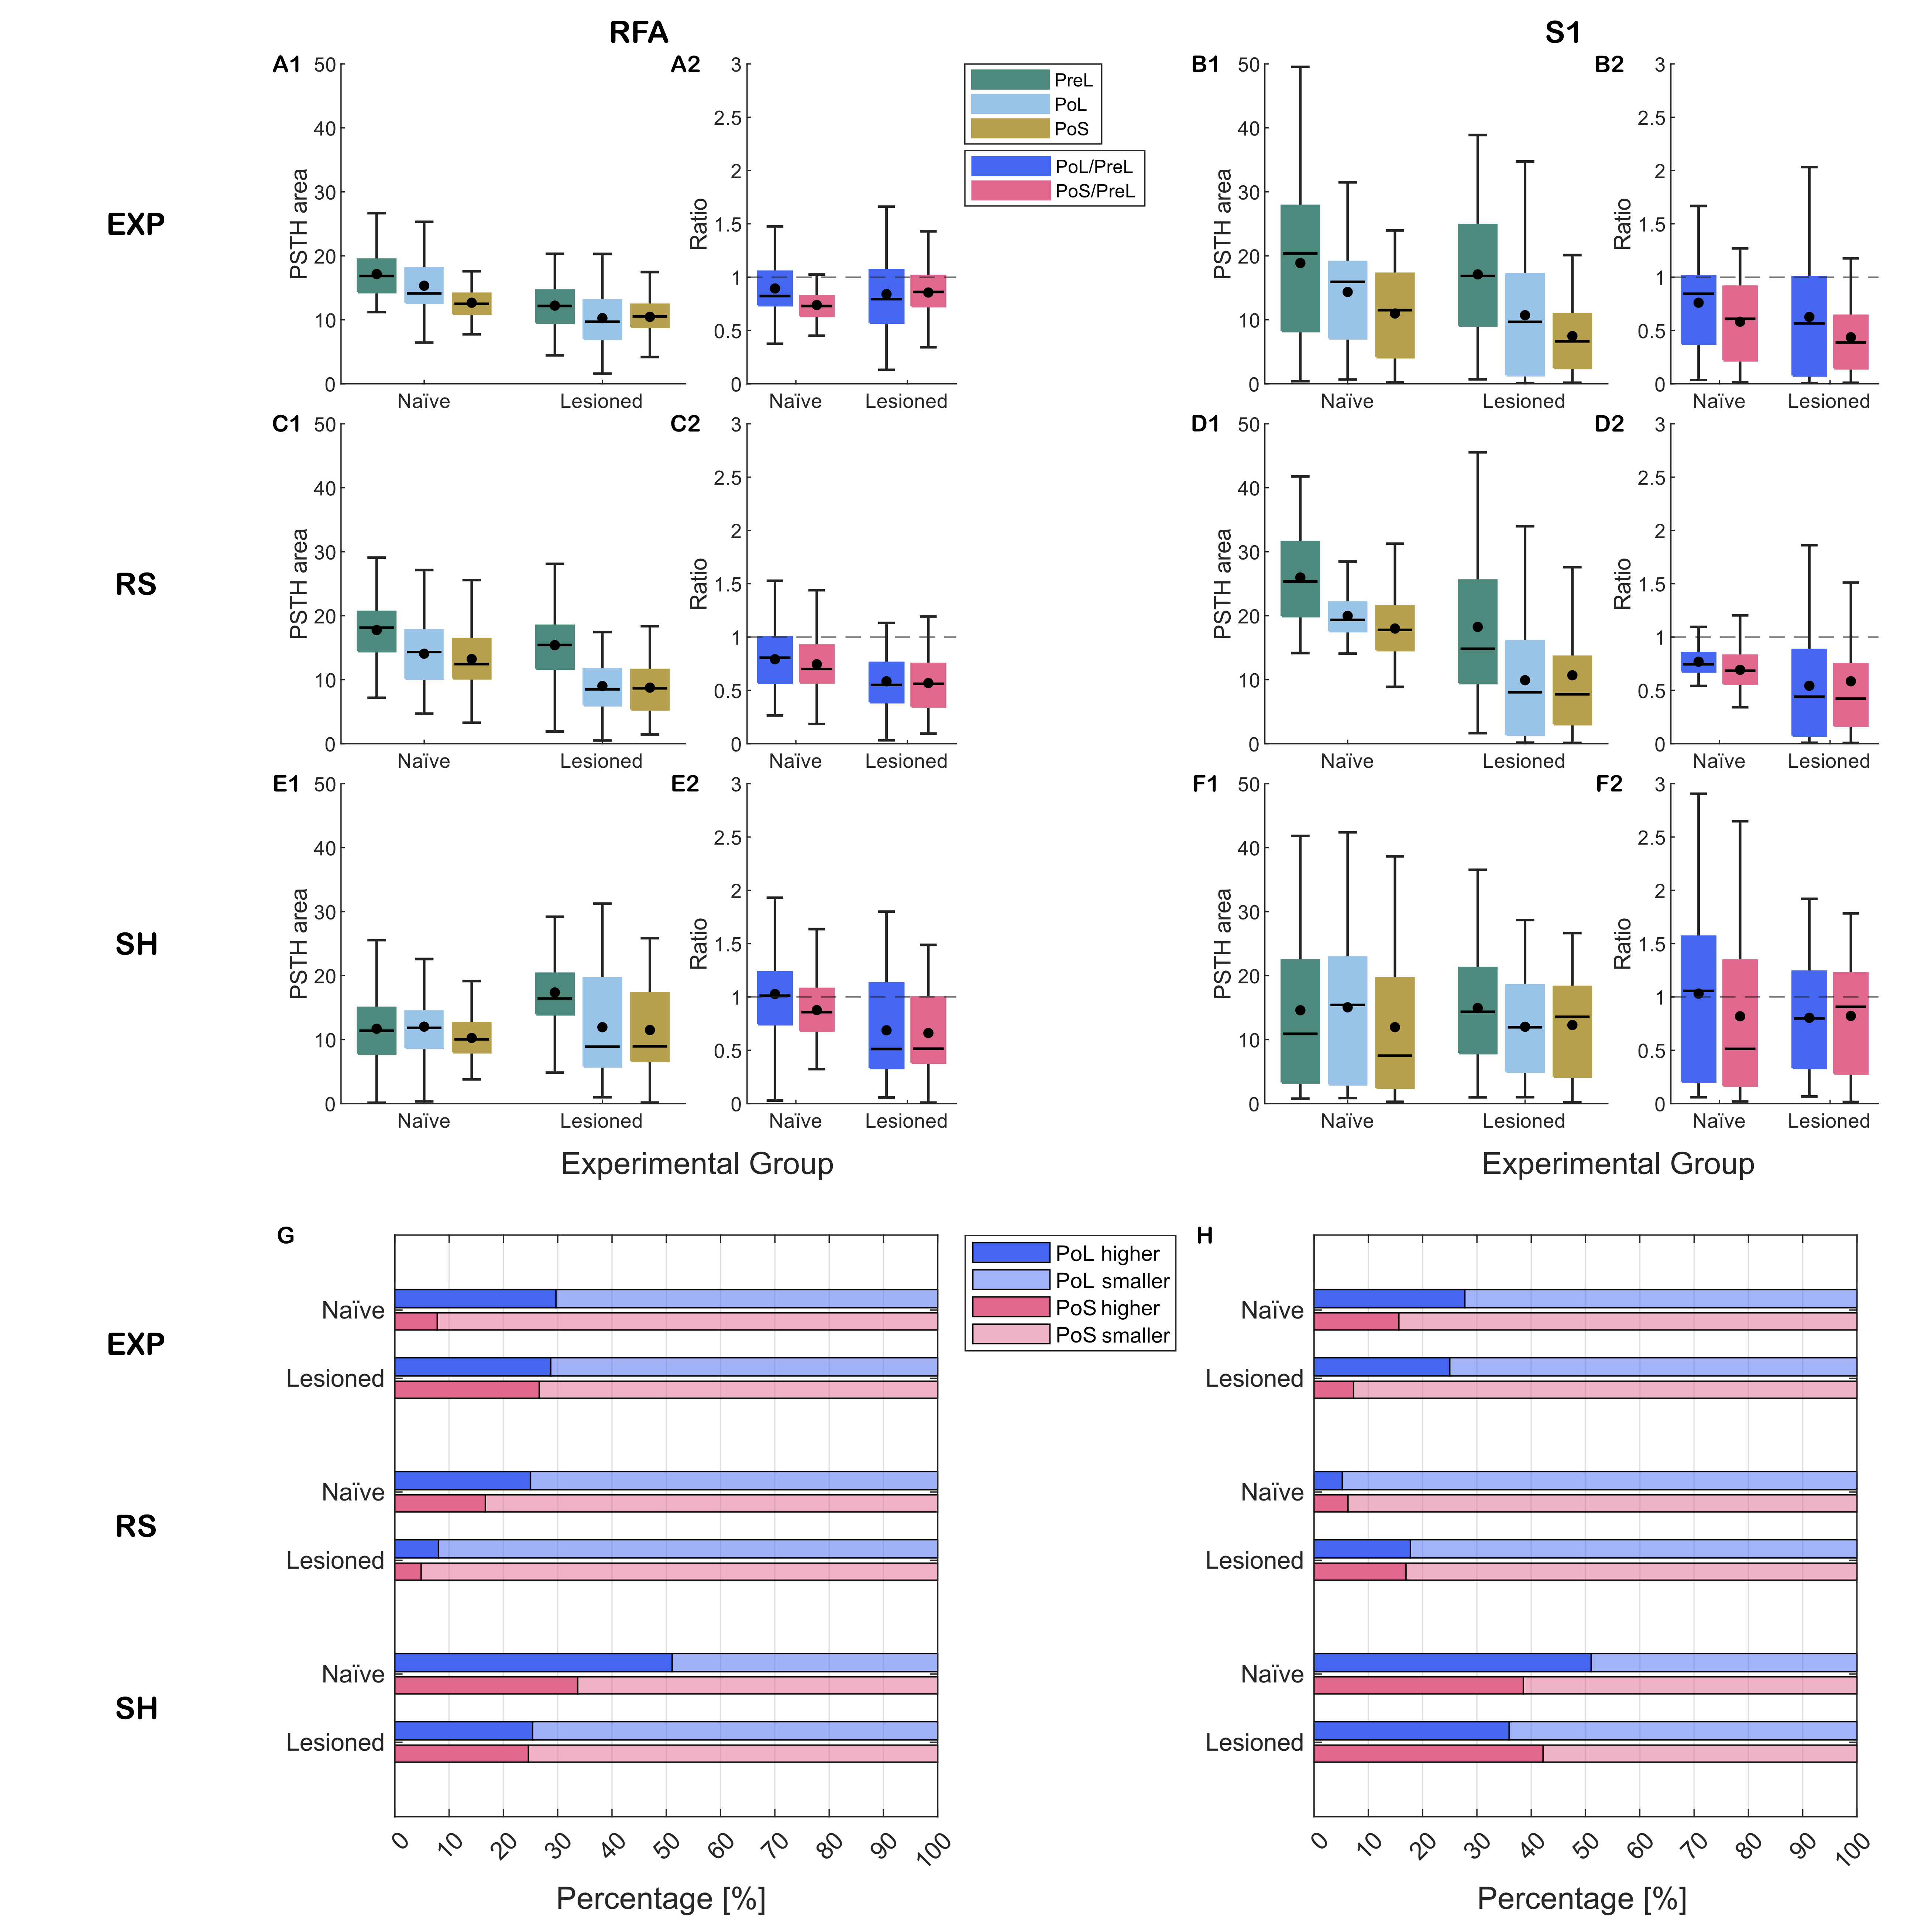
\includegraphics[width=\linewidth]{Figure/Ratio PSTH area separate/ratio all PSTH area 0.2Hz.jpg}
    \end{center}
\end{figure}
\begin{figure}[p!]
    \caption{(figure in the previous page) Effect of lesion and OL stimulations on the evoked response (Connectivity Mapping stimulation 0.2Hz). (A, C, E) Box plot of the PSTH area of RFA for the entire dataset of Naïve and Lesioned rats stimulated with an OL (EXP, RS, SH) paradigm. (B, D, F) Box plot of the PSTH area of S1 for the entire dataset of Naïve and Lesioned rats stimulated with an OL (EXP, RS, SH) paradigm. (A2, B2, C2, D2, E2, F2) Box plot of the ratio between the PSTH area of the PoL and PoS phases with the mean PSTH area of the PreL phase. For each box plot (A - F), the central black line indicates the median, the central black dot indicates the mean and the box limits indicate the 25th and 75th percentiles. The whiskers show the Q1-1.5*IQR and Q3+1.5*IQR, where Q1 and Q3 are the first and third quartiles, while the IQR is the interquartile range (the distance between Q1 and Q3). (G, H) Bar plot of the percentage of channels of RFA and S1 that has an PSTH area in the PoL and PoS phases greater than the mean PSTH area in the PreL phase, for the entire dataset of Naïve and Lesioned rats stimulated with an OL (EXP, RS, SH) paradigm.}
    \label{fig:ratio all PSTH area 0.2Hz}
\end{figure}
\clearpage

\begin{figure}[htp]
    \begin{center}
    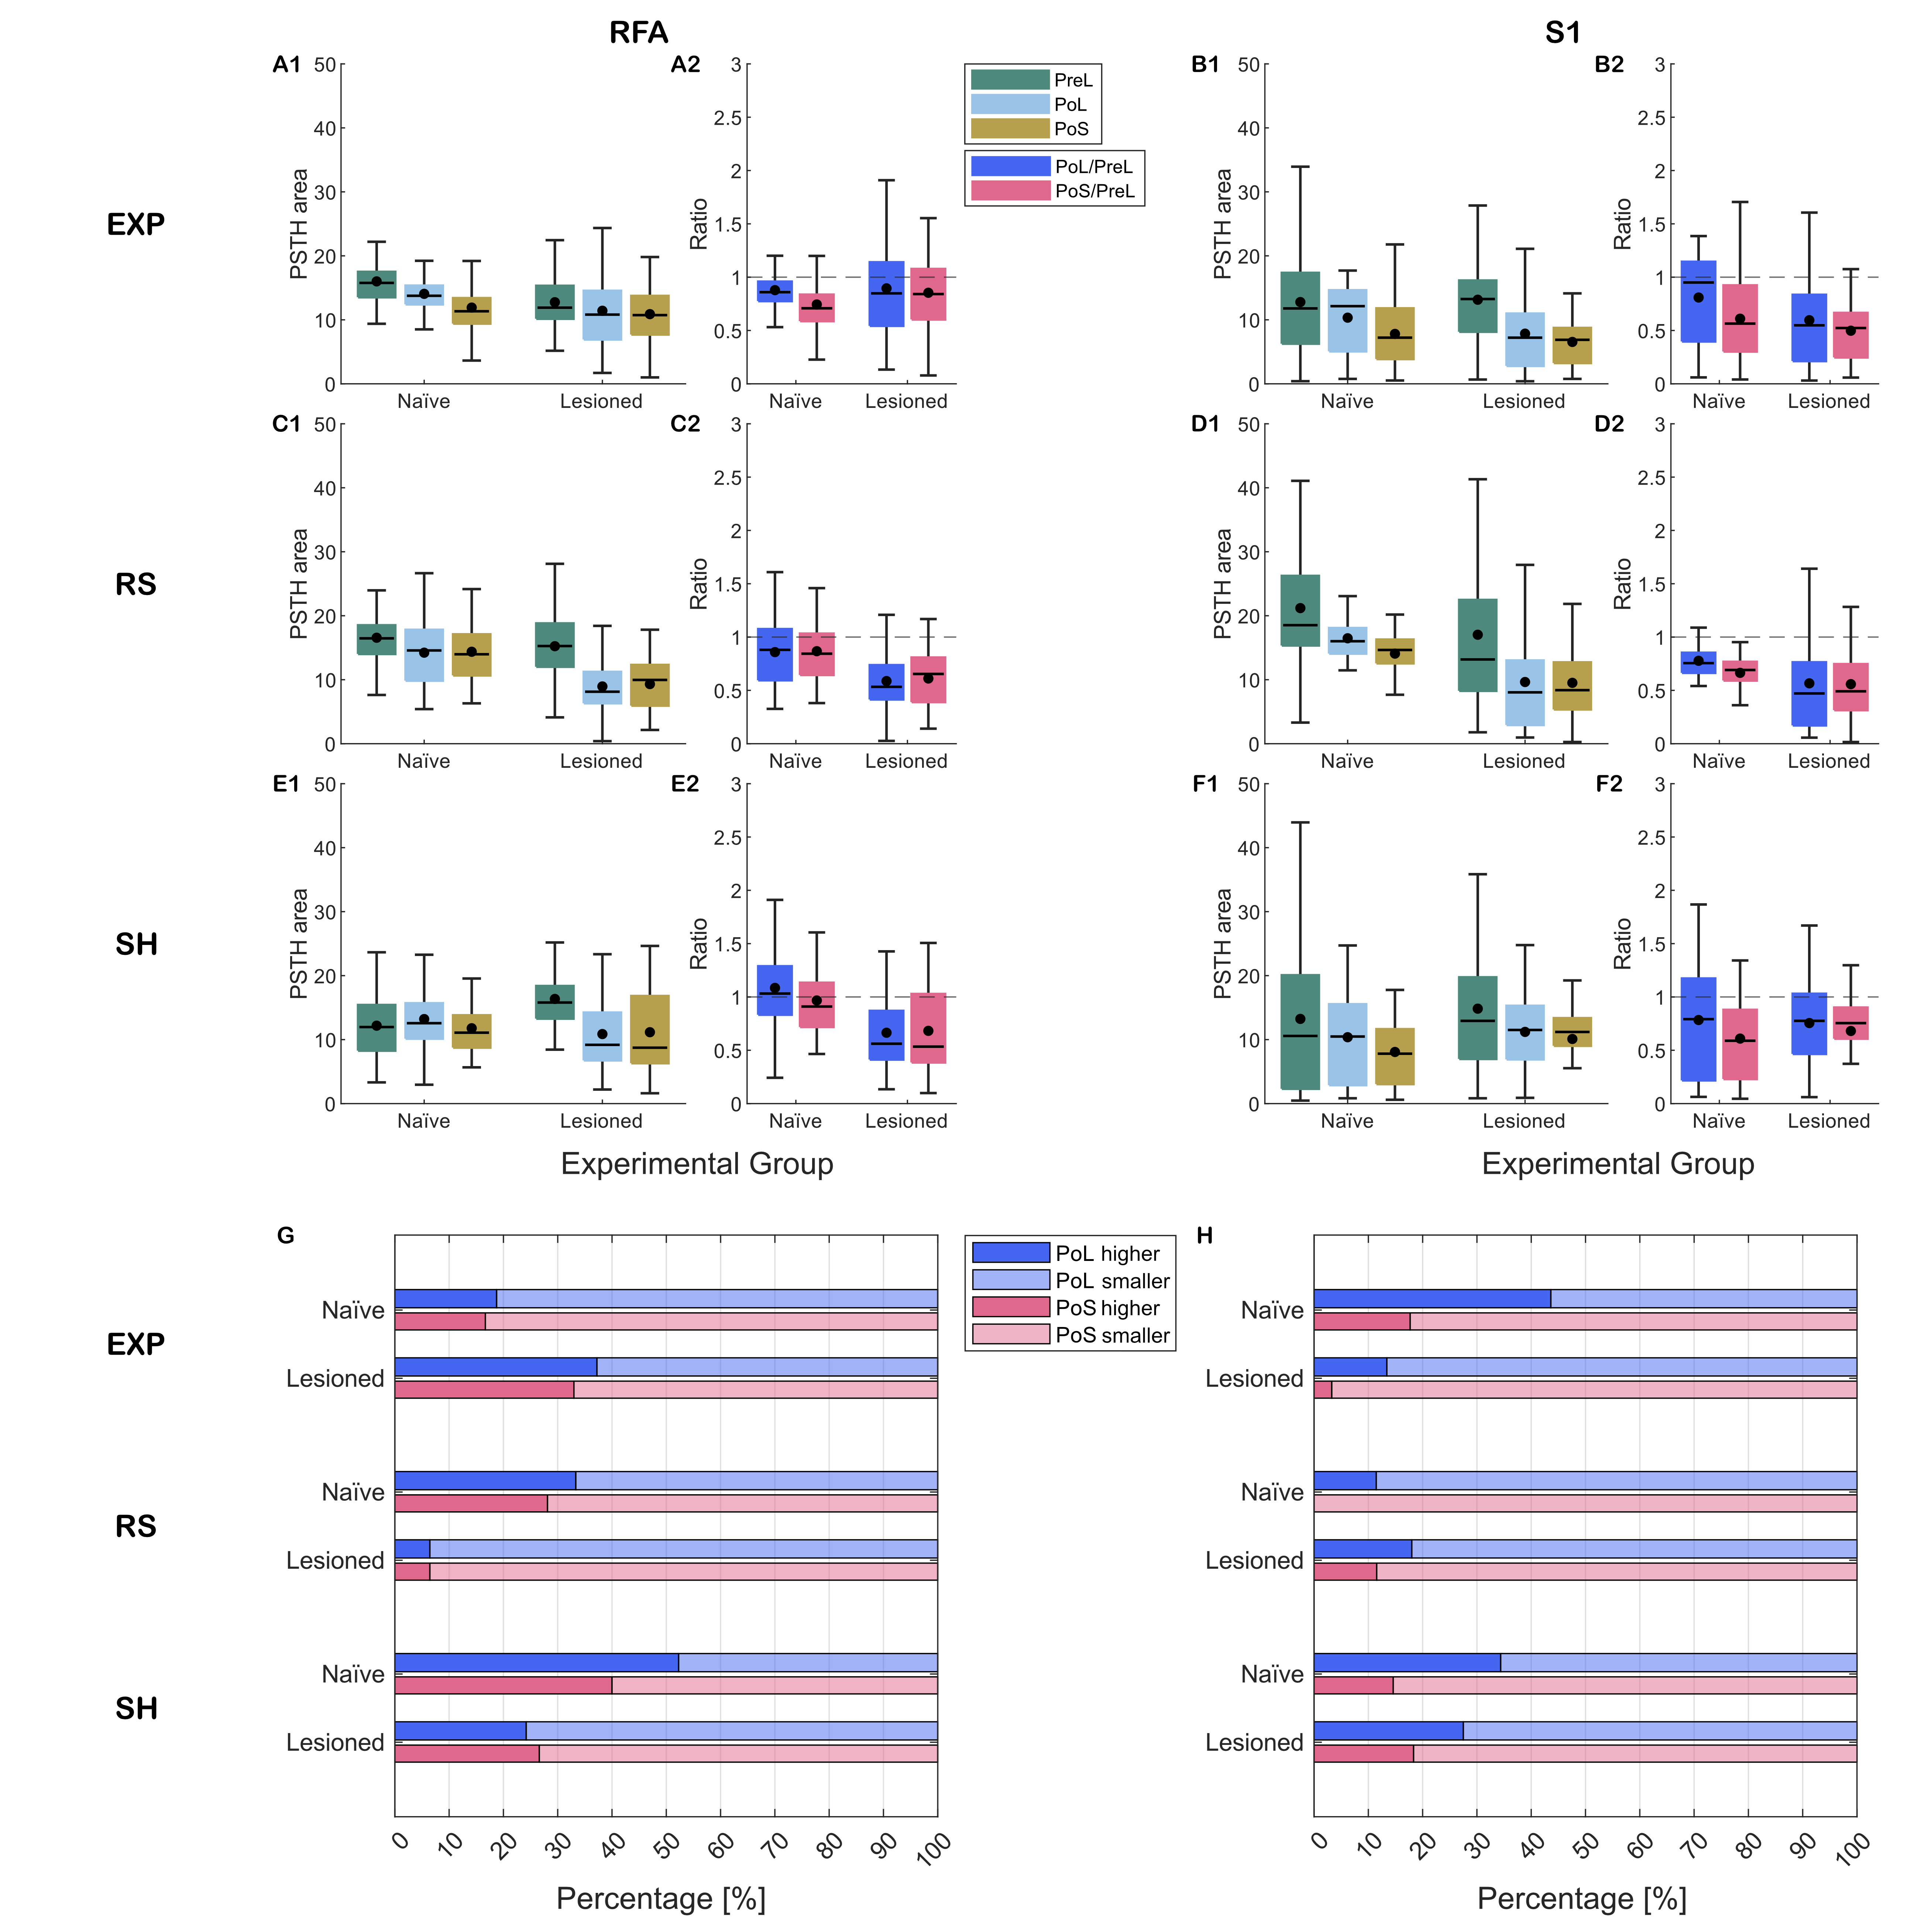
\includegraphics[width=\linewidth]{Figure/Ratio PSTH area separate/ratio all PSTH area 1Hz.jpg}
    \end{center}
\end{figure}
\begin{figure}[p!]
    \caption{(figure in the previous page) Effect of lesion and OL stimulations on the evoked response (Connectivity Mapping stimulation 1Hz). (A, C, E) Box plot of the PSTH area of RFA for the entire dataset of Naïve and Lesioned rats stimulated with an OL (EXP, RS, SH) paradigm. (B, D, F) Box plot of the PSTH area of S1 for the entire dataset of Naïve and Lesioned rats stimulated with an OL (EXP, RS, SH) paradigm. (A2, B2, C2, D2, E2, F2) Box plot of the ratio between the PSTH area of the PoL and PoS phases with the mean PSTH area of the PreL phase. For each box plot (A - F), the central black line indicates the median, the central black dot indicates the mean and the box limits indicate the 25th and 75th percentiles. The whiskers show the Q1-1.5*IQR and Q3+1.5*IQR, where Q1 and Q3 are the first and third quartiles, while the IQR is the interquartile range (the distance between Q1 and Q3). (G, H) Bar plot of the percentage of channels of RFA and S1 that has an PSTH area in the PoL and PoS phases greater than the mean PSTH area in the PreL phase, for the entire dataset of Naïve and Lesioned rats stimulated with an OL (EXP, RS, SH) paradigm.}
    \label{fig:ratio all PSTH area 1Hz}
\end{figure}

\clearpage
\section{Discussion and Conclusion}

In this work, the electrophysiological activity of both the premotor (RFA) and somatosensory (S1) cortex in anesthetized rats affected by a focal lesion in the motor area (M1) was analyzed. The impact of the lesion and subsequent neuromodulation therapies on the evoked responses was evaluated through the computation of the Post-Stimulus Time Histogram (PSTH).

It has been observed that the lesion results in a greater decrease in evoked activity compared to the Naïve group. The CL: ADS paradigm was the only one that led to an increase in evoked activity in the PoS period with respect to the PreL, eventhough it was applied to the Naïve rats. On the other hand, all the open loop stimulation paradigms produced a further decrease of the evoked activity in all Naïve animals, and also in the lesioned ones, except for the OL: SH group.

This preliminary analysis was a necessary step to assess the effectiveness of a new form of neuromodulation therapy, where an open loop system will be utilized to deliver personalized stimulation.

\newpage
\chapter[Tuning the parameters of the SNN]{Tuning the parameters of the SNN\raisebox{.15\baselineskip}{\Large\footnotemark}}
\footnotetext{The results of this chapter were submitted as \textit{Recapitulating the electrophysiological features of in vivo biological networks by using a real-time hardware Spiking Neural Network} for the EMBC 2024 conference. The analysis conducted here is also included in the article titled \textit{BiœmuS: A New Tool for Studying Neurological Disorders Through Real-Time Emulation and Hybridization Using Biomimetic Spiking Neural Networks}, currently under review for publication in Nature Communications.}

\section{Introduction}

This work aims to advance the development of a device for delivering a novel personalized stimulation for post-stroke rehabilitation. As seen before, a promising therapy involves electrical stimulation to establish new connections between separated brain regions, leveraging neural plasticity. Closed-loop stimulation has shown promise in restoring lost abilities in rats \cite{Guggenmos2013,Averna2020,Averna2021}, unlike traditional open-loop paradigms.

This study proposes a tuning phase of a hardware-based SNN \cite{Beaubois2023} for a new open-loop approach that maintains the bio-mimetic nature of stimulation. The spontaneous activity of the RFA area of six healthy adult anesthetized rats was analyzed to extract key electrophysiological features required for customizing SNN parameters (Figure \ref{fig:Biomimetic Approach}).

Various SNNs were built, and comparative analyses between the electrical patterns generated by SNNs and the neural activity recorded from the BNNs were performed. By identifying the SNN that best matches the pool of electrophysiological features observed in vivo, in the future, it may be possible to stimulate the S1 area with a pattern derived from the activity of the digital twin of a BNN.

\begin{figure}[ht!]
    \begin{center}
    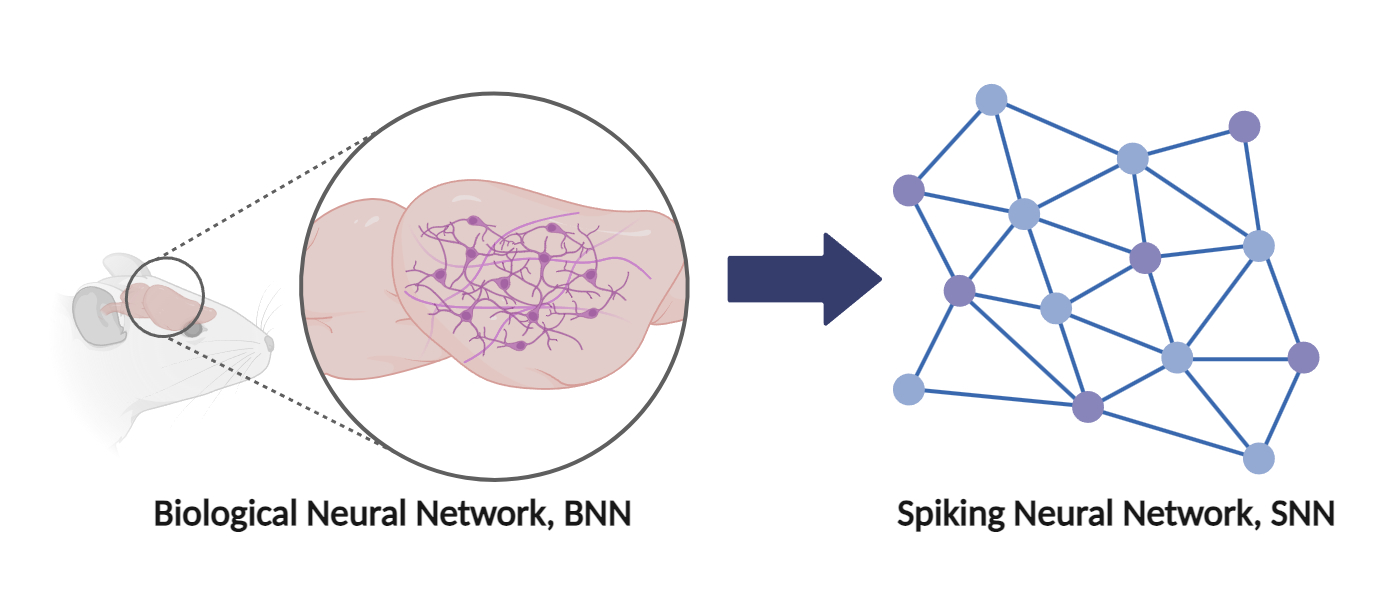
\includegraphics[width=0.9\linewidth]{Figure/Biomimetic Approach.jpg}
    \end{center}
    \caption{Schematic representation of the bio-mimetic approach (from BNN to SNN).}
    \label{fig:Biomimetic Approach}
\end{figure}

\section{Materials and Methods}

\subsection{Biological Neural Network (BNN)}

The biological model that constitutes the Biological Neural Network is derived solely from the RFA area of six animals, chosen based on the shape of their ISIH through visual inspection among those introduced in the previous chapter. Specifically, for the subsequent analyses, only the first 10 minutes of spontaneous activity recorded in the PreL phase of the experimental procedure, outlined in the section "Experimental Protocol" of the previous chapter, are considered to characterize the behavior of a healthy network.

\subsection{Spiking Neural Network (SNN)}

The digital platform employed for the development of the bio-mimetic SNN is a System on Chip (SoC) FPGA based on the Zynq™ UltraScale+ MPSoC architecture (Figure \ref{fig:SoC FPGA}). This platform integrates CPU cores, referred to as software part, and programmable logic (FPGA), referred to as hardware part \cite{Beaubois2023}, on the same chip. 

\begin{figure}[ht!]
    \begin{center}
    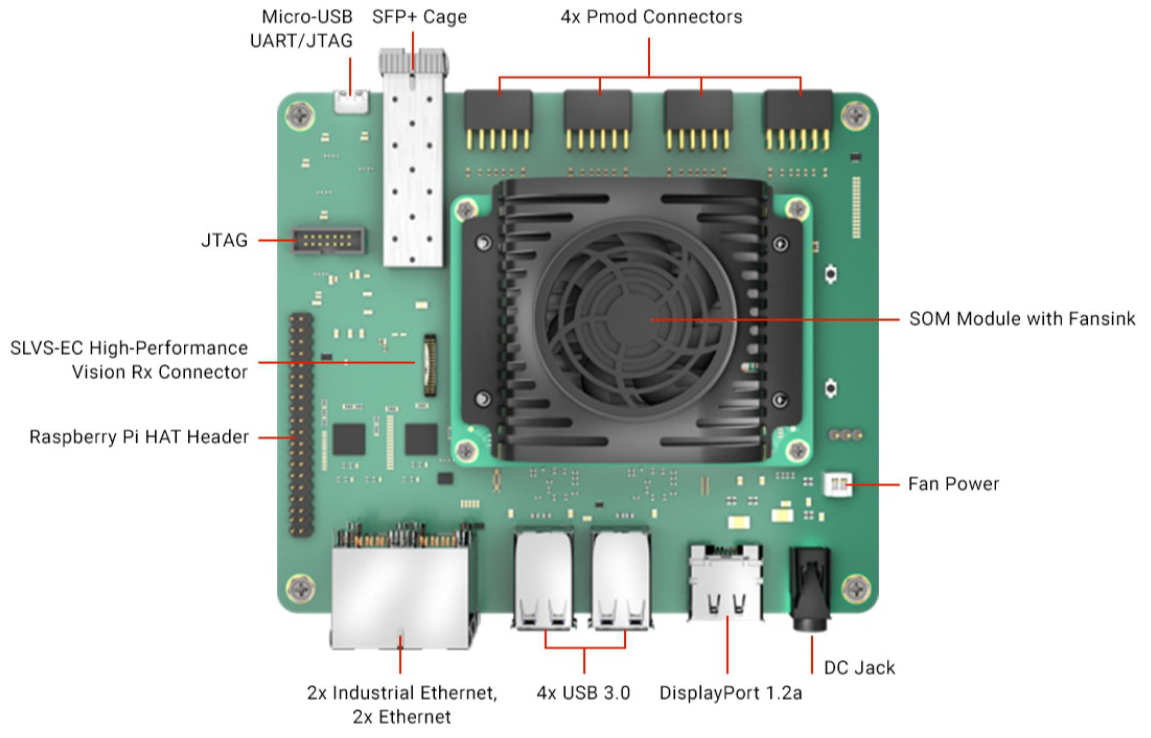
\includegraphics[width=0.9\linewidth]{Figure/SoC FPGA.jpg}
    \end{center}
    \caption{Kria K26 SOM from AMD Xilinx embedded on the development platforms Kria KR260 Robotics Starter Kit. From [https://www.amd.com/en/products/system-on-modules/kria/k26/kr260-robotics-starter-kit.html].}
    \label{fig:SoC FPGA}
\end{figure}

The compact design of the carrier boards, coupled with their flexibility and high processing performance, presents notable advantages for integration into a biohybrid experimental setup.

The system used, capable of running up to 1024 single-compartment neurons fully connected and supporting a total of 2\textsuperscript{20} synapses, is named Bi{\oe}muS, which stands for "\textbf{BIO}mimetic \textbf{EMU}lation \textbf{S}ingle compartment." It incorporates on-board monitoring and provides versatile external communication options, such as Ethernet or WiFi. 

Python scripts enable the configuration and monitoring of the system. They generate two files - one for hardware and one for software configuration of the SoC FPGA (see Figure \ref{fig:Architecture BioEmus}). The software configuration is specified by the file in JSON format (e.g. \textit{swconfig.json}), encompassing various parameters like the path to the hardware configuration file, emulation time, configuration of different monitoring channels, and stimulation step settings. The hardware configuration is determined by the file in txt format (e.g. \textit{hwconfig.txt}), containing various network parameters such as the Hodgkin-Huxley model, synaptic connections and weights, ion rates tables, and monitoring properties.

\begin{figure}[ht!]
    \begin{center}
    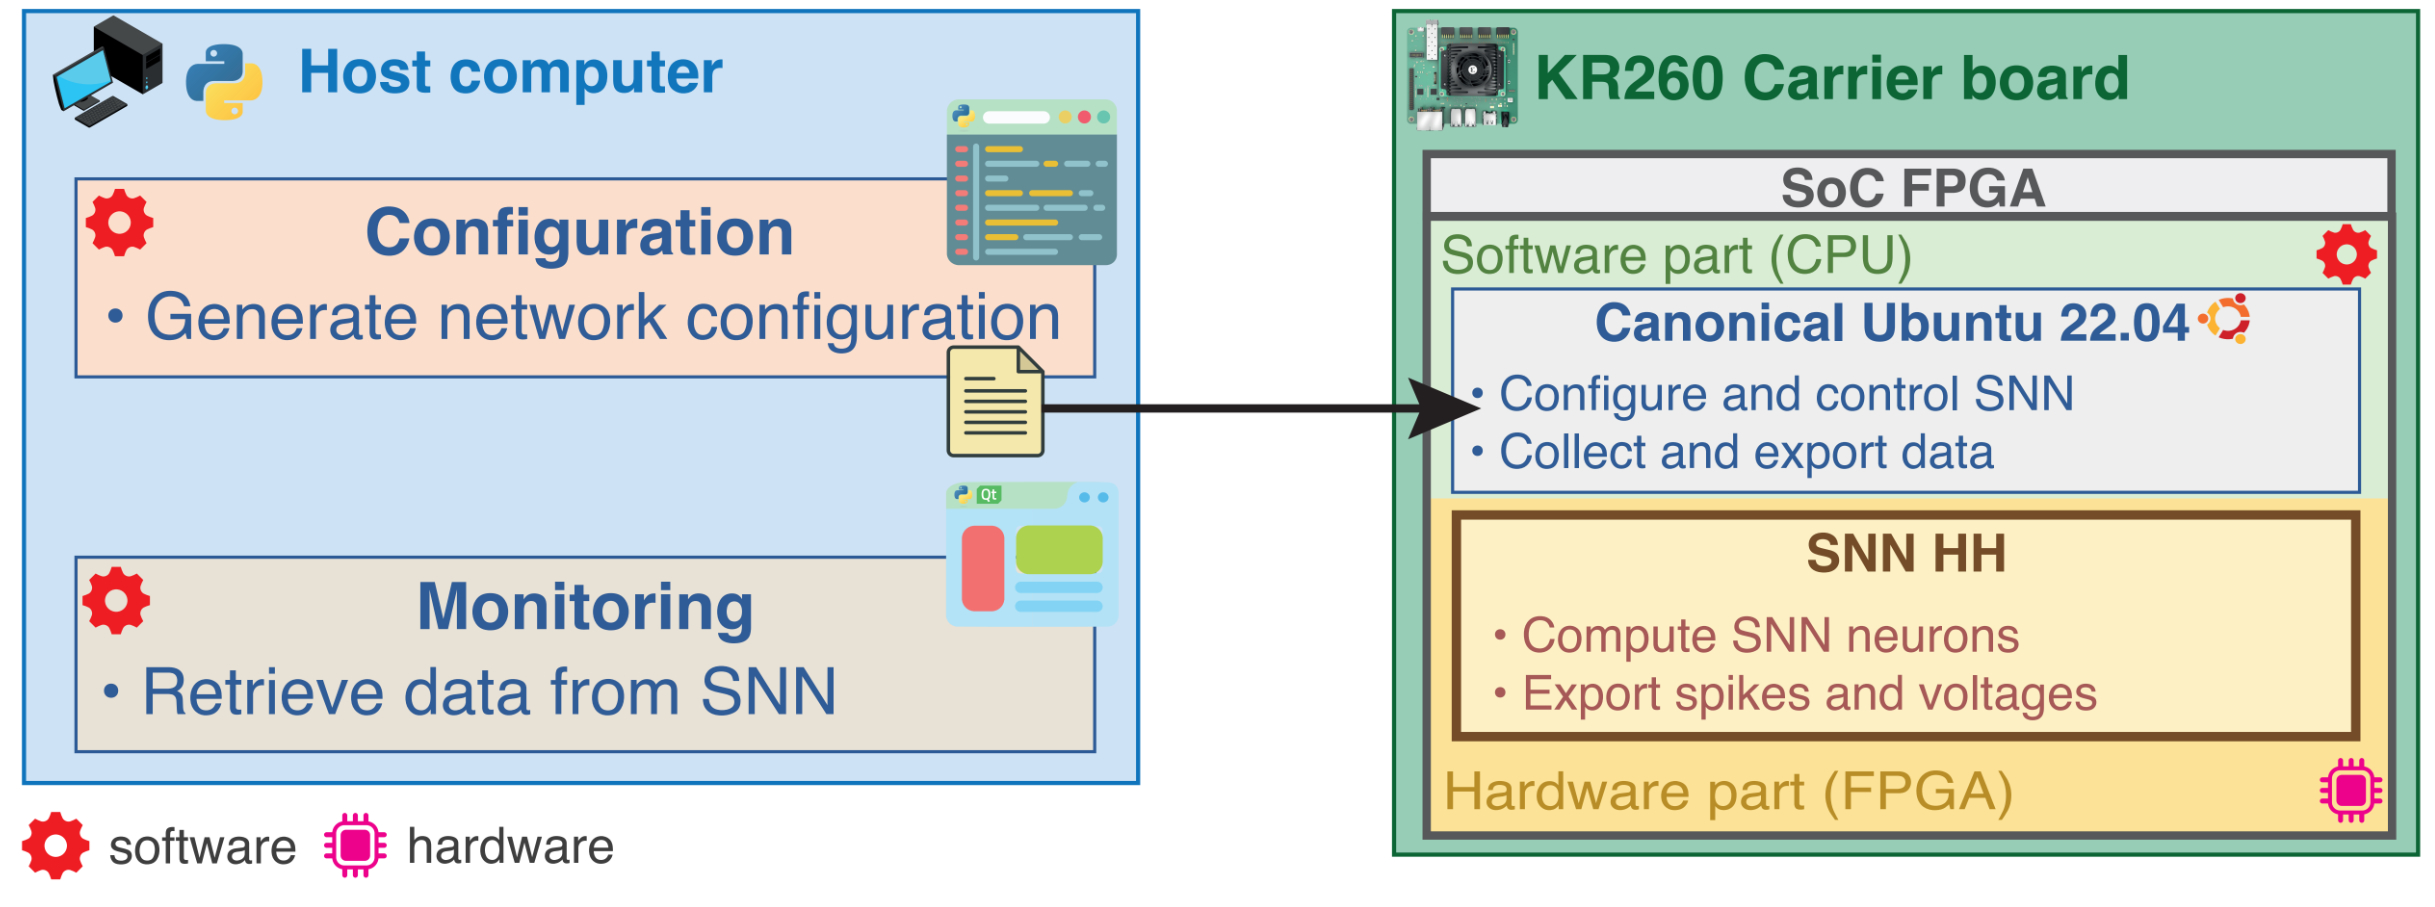
\includegraphics[width=0.9\linewidth]{Figure/Architecture BioEmus.jpg}
    \end{center}
    \caption{Block diagram illustrating the architecture of BioemuS and distinguishing between software and hardware designs through red and pink symbols, respectively.}
    \label{fig:Architecture BioEmus}
\end{figure}

The SNN utilizes Hodgkin-Huxley (HH) neurons \cite{HodgkinHuxley1990}, with preset neuron types including Fast Spiking (FS) and Regular Spiking (RS) neurons (parameters in Table \ref{tab:Neurons and Noise Parameters}; also, refer to Intrinsically Bursting and Low Threshold Spiking neurons, which are not used in this thesis work). Additionally, a biomimetic current simulating synaptic noise, based on the Ornstein-Uhlenbeck process \cite{Destexhe2001} as described by \cite{Khoyratee2019}, is employed to replicate spontaneous activity within the network neurons (parameters in Table \ref{tab:Neurons and Noise Parameters}). 

\begin{table}[!ht]
\centering
\small
\tabcolsep=0.11cm
\begin{tabular}{lccccc}
\hline Parameter & FS & RS & IB & LTS & Unit \\
\hline$g_{N a}$ & 0.05 & 0.05 & 0.05 & 0.05 & $S / \mathrm{cm}^2$ \\
$g_K$ & 0.01 & 0.005 & 0.005 & 0.005 & $S / \mathrm{cm}^2$ \\
$g_M$ & 0.0 & $7 \times 10^{-5}$ & $3 \times 10^{-5}$ & $3 \times 10^{-5}$ & $\mathrm{~S} / \mathrm{cm}^2$ \\
$g_L$ & 0.0 & 0.0 & $1 \times 10^{-4}$ & 0.0 & $\mathrm{~S} / \mathrm{cm}^2$ \\
$g_T$ & 0.0 & 0.0 & 0.0 & $4 \times 10^{-4}$ & $\mathrm{~S} / \mathrm{cm}^2$ \\
$g_{\text {Leak }}$ & 0.00015 & 0.0001 & $1 \times 10^{-5}$ & $1 \times 10^{-5}$ & $\mathrm{~S} / \mathrm{cm}^2$ \\
$E_{N a}$ & 50.0 & 50.0 & 50.0 & 50.0 & $\mathrm{mV}$ \\
$E_K$ & -100.0 & -100.0 & -90.0 & -100.0 & $\mathrm{mV}$ \\
$E_{\text {Ca }}$ & 0.0 & 0.0 & 120.0 & 120.0 & $\mathrm{mV}$ \\
$E_{\text {Leak }}$ & -70.0 & -70.0 & -70.0 & -75.0 & $\mathrm{mV}$ \\
$v_{\text {init }}$ & -70.0 & -70.0 & -70.0 & -75.0 & $\mathrm{mV}$ \\
$\mu_{\text {noise }}$ & 0.048 & 0.042 & 0.042 & 0.042 & 1 \\
$\theta_{\text {noise }}$ & 8.0 & 8.0 & 8.0 & 8.0 & 1 \\
$\sigma_{\text {noise }}$ & 0.11 & 0.09 & 0.09 & 0.09 & 1 \\
$I_{\text {stim }}$ & 0.03 & 0.03 & 0.03 & 0.03 & $\mathrm{~mA} / \mathrm{cm}^2$ \\
area & $\left(67 \times 10^{-4}\right)^2$ & $\left(96 \times 10^{-4}\right)^2$ & $\left(96 \times 10^{-4}\right)^2$ & $\left(96 \times 10^{-4}\right)^2$ & $\mathrm{~cm}^2$ \\
$c_{\text {mem }}$ & 1.0 & 1.0 & 1.0 & 1.0 & $\mu \mathrm{F} / \mathrm{cm}^2$ \\
\hline
\end{tabular}
\caption{Parameters of the HH model and noise for the 4 preset types of neurons tunable from the Python scripts.}
\label{tab:Neurons and Noise Parameters}
\end{table}

Fast and slow excitation and inhibition synapses (AMPAR, NMDAR, GABA\textsubscript{A}R, GABA\textsubscript{B}R) connect neurons in the SNN, with parameters detailed in Table \ref{tab:Synapses Parameters}. 

\begin{table}[!ht]
\centering
\small
\tabcolsep=0.11cm
\begin{tabular}{lccccc}
\hline Parameter & AMPAR & NMDAR & GABA$_{\mathrm{A}} \mathrm{R}$ & GABA$_{\mathrm{B}} \mathrm{R}$ & Unit \\
\hline$g$ & 0.35 & 0.3 & 0.25 & 1.0 & $n S$ \\
$E$ & 0 & 0 & -80 & -95 & $\mathrm{mV}$ \\
$\alpha$ & $1.1 \times 10^6$ & $7.2 \times 10^6$ & $5 \times 10^6$ & - & $\mathrm{M}^{-1} \mathrm{sec}^{-1}$ \\
$\beta$ & 190 & 6.6 & 180 & - & $\mathrm{sec}^{-1}$ \\
$K_1$ & - & - & - & $9 \times 10^4$ & $\mathrm{M}^{-1} \mathrm{sec}^{-1}$ \\
$K_2$ & - & - & - & 1.2 & $\mathrm{sec}^{-1}$ \\
$K_3$ & - & - & - & 180 & $\mathrm{sec}^{-1}$ \\
$K_4$ & - & - & - & 34 & $\mathrm{sec}^{-1}$ \\
$K_d$ & - & - & - & 100 & $\mu M^4$ \\
$n$ & - & - & - & 4 & 1 \\
\hline
\end{tabular}
\caption{Parameters of the 4 types of synapses tunable from the Python scripts.}
\label{tab:Synapses Parameters}
\end{table}

Moreover, the configuration scripts allowed the setup of the ratio between excitatory and inhibitory neurons, the ratio between fast and slow synapses, the synaptic weight, and the connection probability between neurons, according to custom equations. Equation \ref{eq:Synaptic Connection Rule} represents the connection rule used to connect two neurons and illustrates how the connection probability varies linearly based on their distance from each other:

\begin{equation}
p = p_{max} (1-\frac{d_{npre-npost}}{d_{net}})
\label{eq:Synaptic Connection Rule}
\end{equation}

where $p$ is the probability of connection between two neurons, $p_{max}$ is the maximum probability of connection between two neurons, $d_{npre-npost}$ is the distance between the presynaptic and postsynaptic neuron, $d_{net}$ is the diameter of the neuronal network. 

Equation \ref{eq:Synaptic Connection Rule}, together with a custom procedure for the cluster-like positioning of the neurons in the network, favored the creation of a network topology resembling the small-world one, with more connections within the same cluster and less between clusters as depicted in Figure \ref{fig:Network Topology}.

\begin{figure}[ht!]
    \begin{center}
    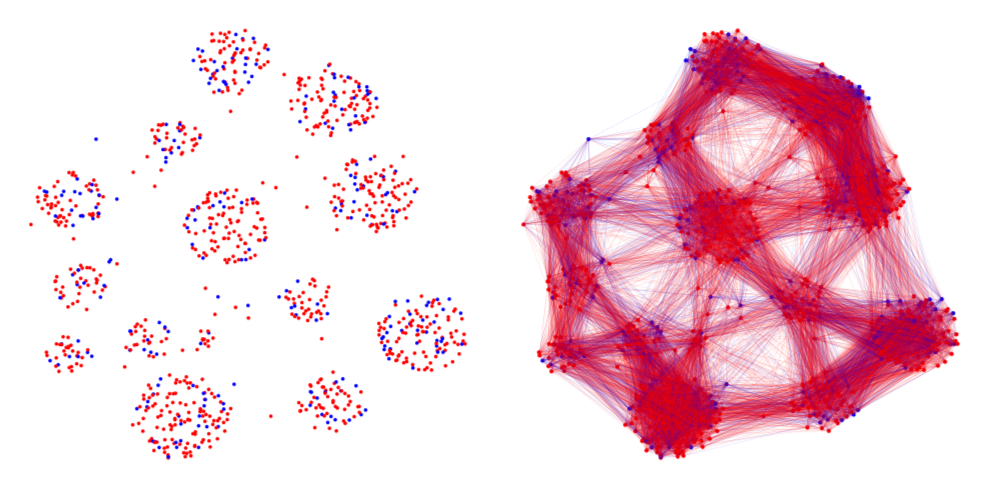
\includegraphics[width=0.9\linewidth]{Figure/Network Topology.jpg}
    \end{center}
    \caption{Position of the neurons (left) and their connections (right) of the simulated network. Blue dots are inhibitory neurons that make inhibitory synapses (blue lines) while red dots are excitatory neurons that make excitatory synapses.}
    \label{fig:Network Topology}
\end{figure}

The time step for the computation of the neuron is 2\textsuperscript{-5} ms, as in \cite{Khoyratee2019}, to ensure satisfactory stability and accuracy in the system solving with Forward Euler solving. Additionally, spikes are compressed over a time stamp of 1 ms, resulting in a spike train with a frequency of 1000 Hz.

In this work, a bank of 325 spiking neural networks, each comprising 1024 neurons, was emulated for 10 minutes each, varying the values of the specified configuration parameters. To maintain consistency in the positions and connections of the network's neurons, a seed was utilized to eliminate variability in the network's topology generation algorithm. This approach ensured a fairer comparison between the networks.

\subsection{Data and Statistical Analyses}

\subsubsection{Data Processing}

All the in-vivo recordings were preprocessed as described in the previous chapter in the section "Preprocessing". The subsequent characterization of the firing activity of both the biological and artificial neural networks was performed using Python. The analyses focused on several biomarkers, including Inter-Spike Interval (ISI, ms), Mean Firing Rate (MFR, spikes/s), Mean Bursting Rate (MBR, bursts/min), Pearson’s Correlation (PC), and Burstiness Index (BI). For these analyses all the detected neurons were considered.

\subsubsection{Mean Firing Rate (MFR)} 

The level of the neuronal firing was evaluated computing the mean firing rate that calculates the average number of spikes in the unit of time (s). 

\subsubsection{Inter-Spike Interval (ISI)}

The inter-spike intervals were analyzed computing the ISI histogram (ISIH) by aggregating the ISIs of all sorted neurons in each network.

\subsubsection{Mean Bursting Rate (MBR)}

The level of the neuronal bursting was evaluated computing the mean bursting rate that calculates the average number of bursts in the unit of time (min). The bursts were detected using the string method (i.e. a max inter-spike interval of 100 ms and 5 as minimum number of intra-burst spikes) according to \cite{Chiappalone2005}.  

\subsubsection{Pearson's Correlation (PC)}

For the computation of the Pearson's coefficient, the method explained in \cite{Selinger2004} was used, with a bin of 200 ms. It's an algorithm that aims to capture the correlation between the neurons of the network.

\subsubsection{Burstiness Index (BI)}

The burstiness index algorithm and its parameters were consistent with those described in \cite{Wagenaar2005}. Its objective is to assess the level of network synchronization without directly analyzing burst activity, thereby circumventing the limitations introduced by burst detection algorithms.

\subsubsection{Statistical Analysis}

The statistical analysis was performed in Python. Only those neurons, either from the SNNs or the six BNNs, with a MFR greater than 0.5 spikes/s were considered for performing the one-way ANOVA test on the log-transformed MFR. P-values were considered significant for $p<0.0001$.

\section{Results}

\subsection{Performances of the simulated SNNs}

A method was devised to identify the most relevant SNN configurations from a range of constructed models. A comparative analysis was carried out between the BNNs, considered as the reference, and the 325 SNNs. This comparison relied on the Root Mean Square deviation (RMSE), calculated between the median inter-spike interval histogram (ISIH) trends of the biological network and the one of each SNN. Additionally, comparisons between the artificial and the biological networks were executed by assessing the differences in the median values of key biomarkers defined in the previous section, i.e. MFR, MBR, PC, and BI. According to this, a grading system was established by computing the absolute value of the distance between each biomarker computed for the SNN and the target value (i.e. the median) of the same biomarker for the BNN. These differences (in absolute values) were then normalized considering the maximum and minimum values of each biomarker among all the configurations, as depicted in the following Equation \ref{eq:Grading Formula}:

\begin{equation}
Grade = 1 - \left[\frac{\left|diff_{i,m}\right|-min(\left|diff_{m}\right|)}{max(\left|diff_{i,m}\right|-min(\left|diff_{m}\right|))}\right] 
\label{eq:Grading Formula}
\end{equation}

where $diff_{i,m}$ is the i-th difference between the m-th biomarker of the i-th SNN configuration and the target value of the same biomarker of the BNN.

By computing all the grades for the several identified biomarkers, the radar plot, depicted in Figure \ref{fig:Radar Plot Grades}, was obtained where the distribution of all the 325 SNN configurations (grey lines) can be appreciated. 

\begin{figure}[ht!]
    \begin{center}
    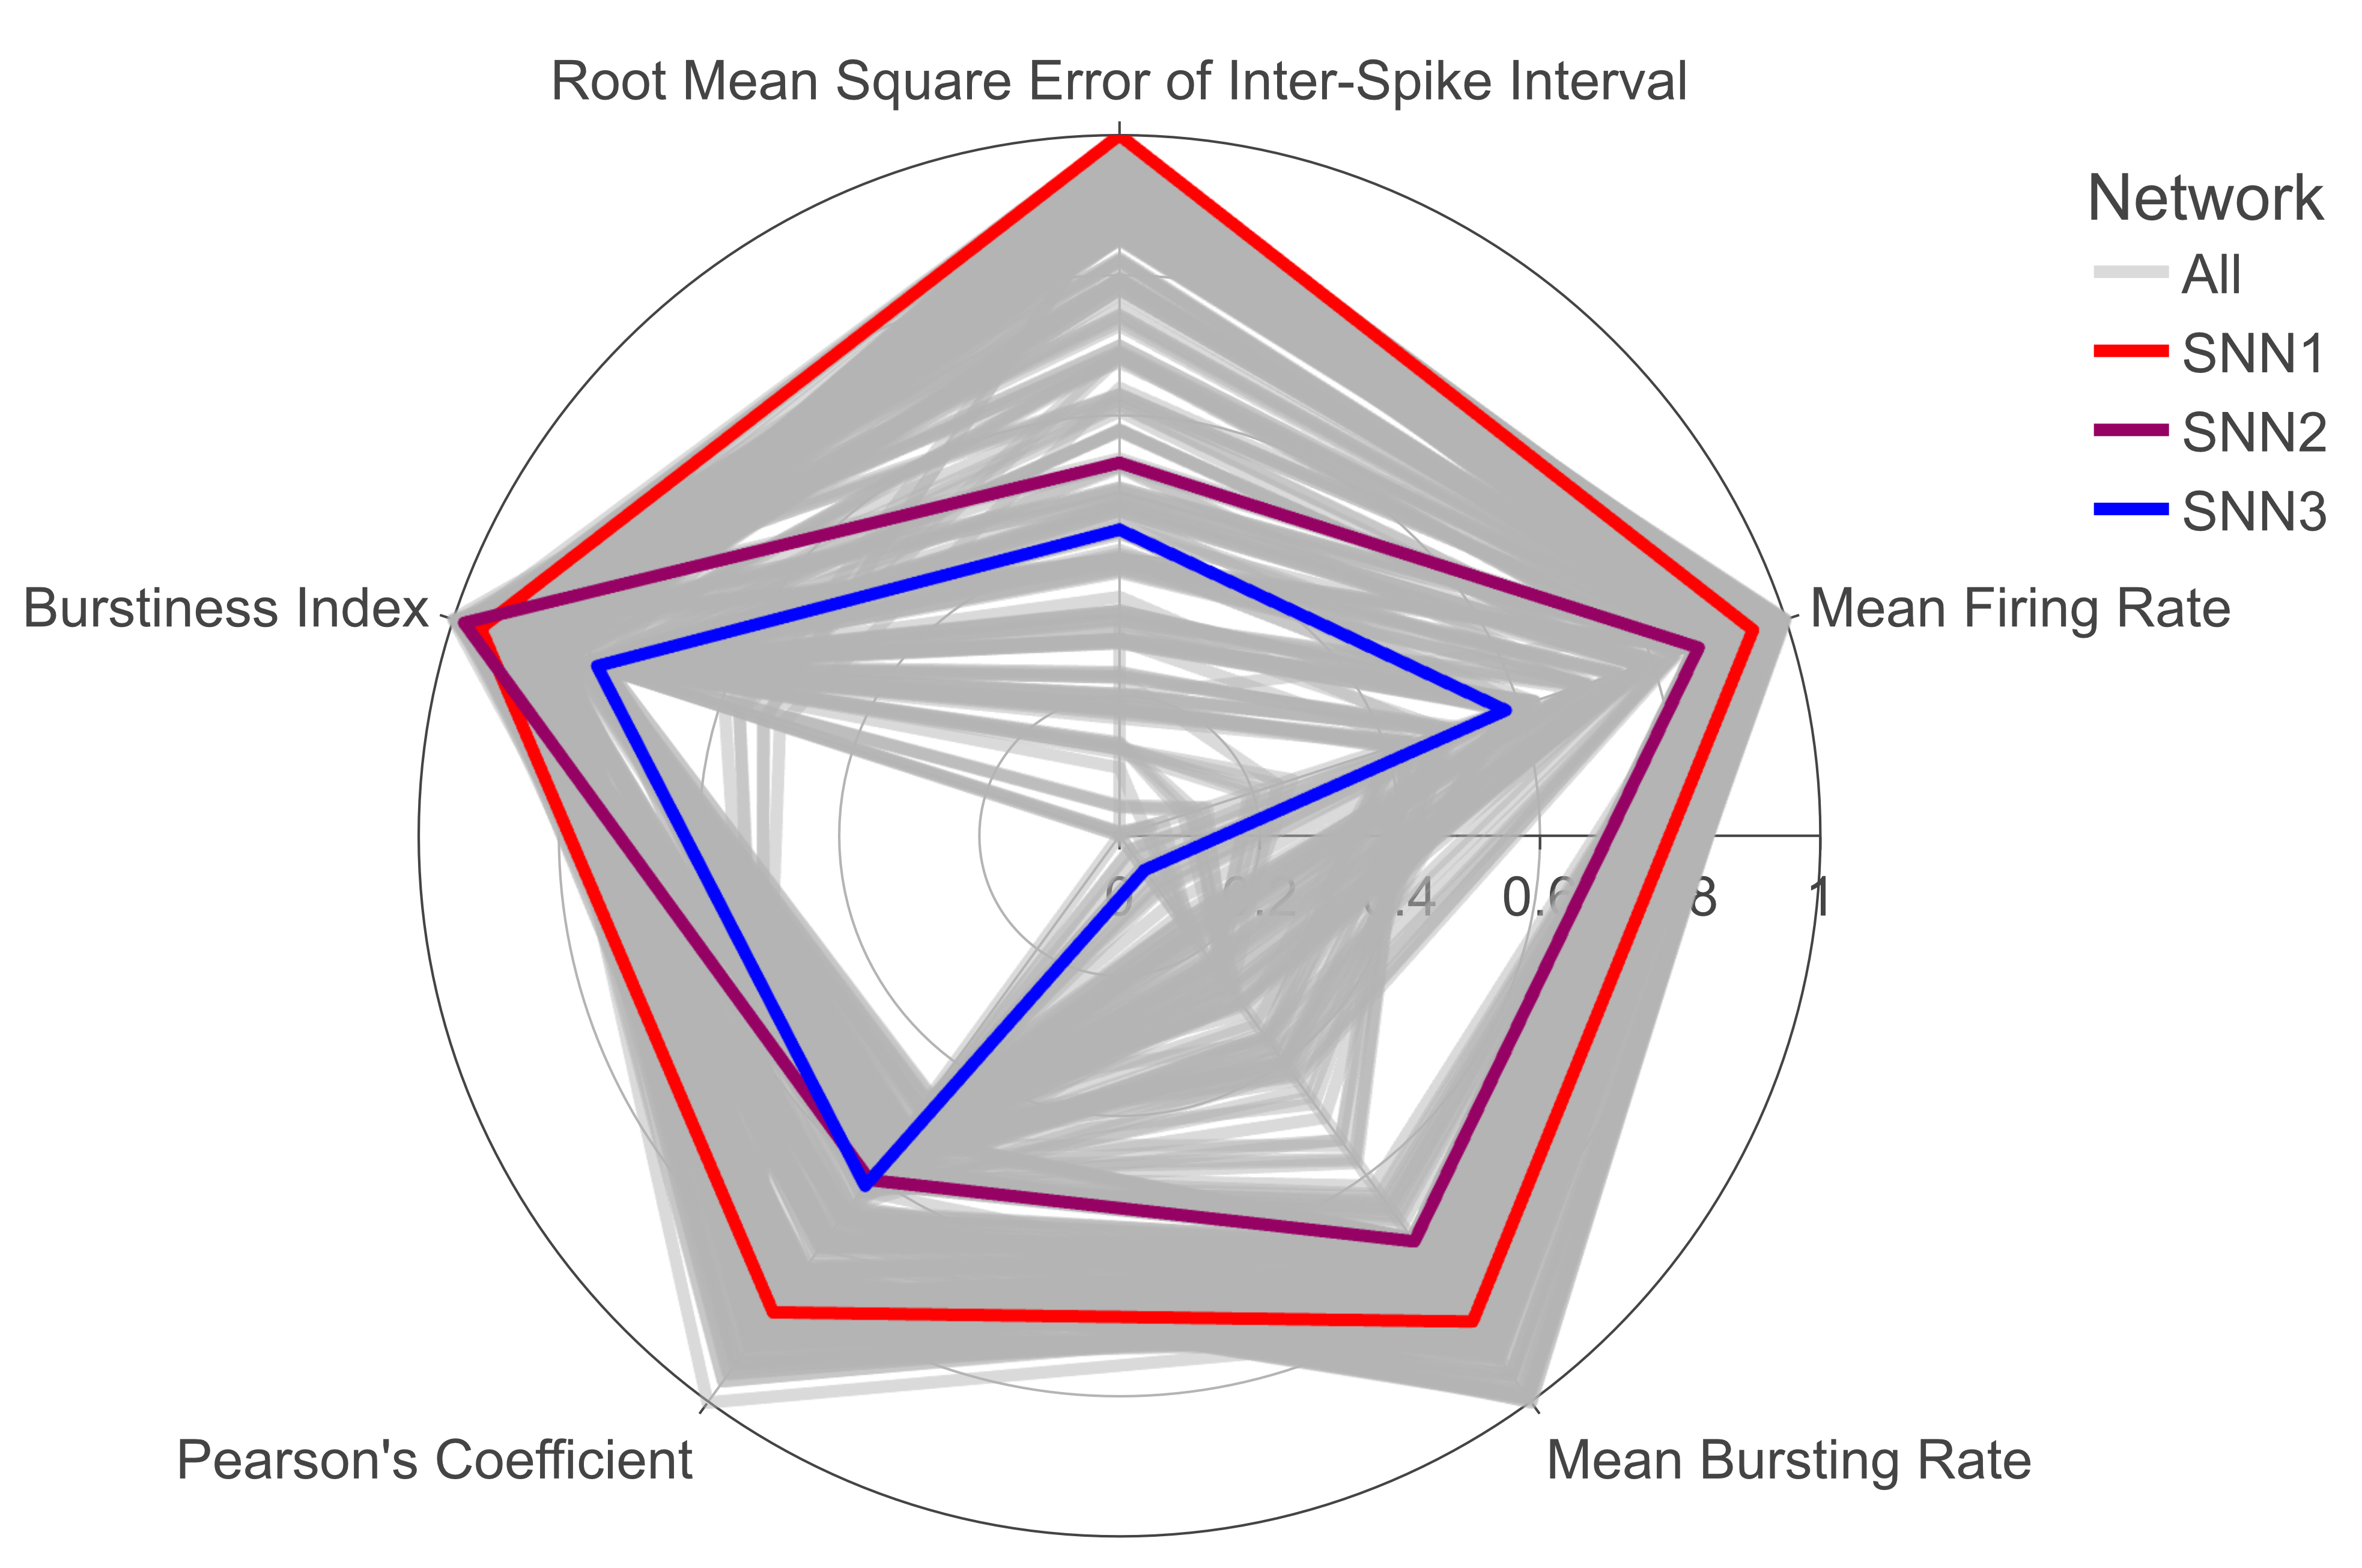
\includegraphics[width=\linewidth]{Figure/Radar Plot Grades.jpg}
    \end{center}
    \caption{Radar plot of the selected network biomarkers, which are: Root Mean Square Error of the Inter Spike Interval (RMSE), Mean Firing Rate (MFR), Mean Bursting Rate (MBR), Pearson’s Coefficient (PC), and Burstiness Index (BI). The plot for each configured SNN is represented in grey. SNN1 is highlighted in red, exhibiting a plot that covers a larger area. SNN2, shown in blue, has a plot covering a median area, while SNN3, depicted in purple, covers one of the smallest areas.}
    \label{fig:Radar Plot Grades}
\end{figure}

Three configurations have been highlighted among all the available: one exemplifying the network with the highest score (SNN1, depicted by the red line), and two additional instances (SNN2 and SNN3, illustrated by the purple and blue lines, respectively) characterized by lower scores, suggesting deviations from the BNN. This choice enabled the assessment of how fine-tuning affects the electrophysiological activity of individual networks.

Ultimately, the overall grade for each specific configuration was established by multiplying each normalized value with respect to various biomarkers, as outlined in Table \ref{tab:Network Performance} for the three selected SNNs. It can be observed that SNN1 obtains the highest score, SNN2 falls in the median range, and SNN3 receives the lowest score among those selected.

\begin{table}[!ht]
\centering
\small
\tabcolsep=0.11cm
\begin{tabular}{|l|c|c|c|c|c|c|}
\hline \multirow{2}{*}{ Network } & \multicolumn{6}{|c|}{ PERFORMANCE VOTE } \\
\cline { 2 - 7 } & MFR & MBR & \begin{tabular}{c} 
RMSE \\
of ISI
\end{tabular} & PC & BI & \begin{tabular}{c} 
FINAL \\
GRADE
\end{tabular} \\
\hline SNN1 & 0.95 & 0.86 & 1 & 0.84 & 0.96 & 0.66 \\
\hline SNN2 & 0.87 & 0.72 & 0.53 & 0.61 & 0.98 & 0.20 \\
\hline SNN3 & 0.58 & 0.6 & 0.44 & 0.62 & 0.78 & 0.01 \\
\hline
\end{tabular}
\caption{Network Performance.}
\label{tab:Network Performance}
\end{table}

\subsection{Comparing artificial and biological neural 
networks}

A comparative study was performed to evaluate the firing dynamics of the selected SNNs and the target BNN. Figure \ref{fig:Histo-Box Comparison SNN-BNN}A reports the ISI histogram profiles of the chosen SNNs (SNN1 in red, SNN2 in purple, SNN3 in blue) and the pool of the six BNNs (in black, with the confidence interval shaded). 

\begin{figure}[ht!]
    \begin{center}
    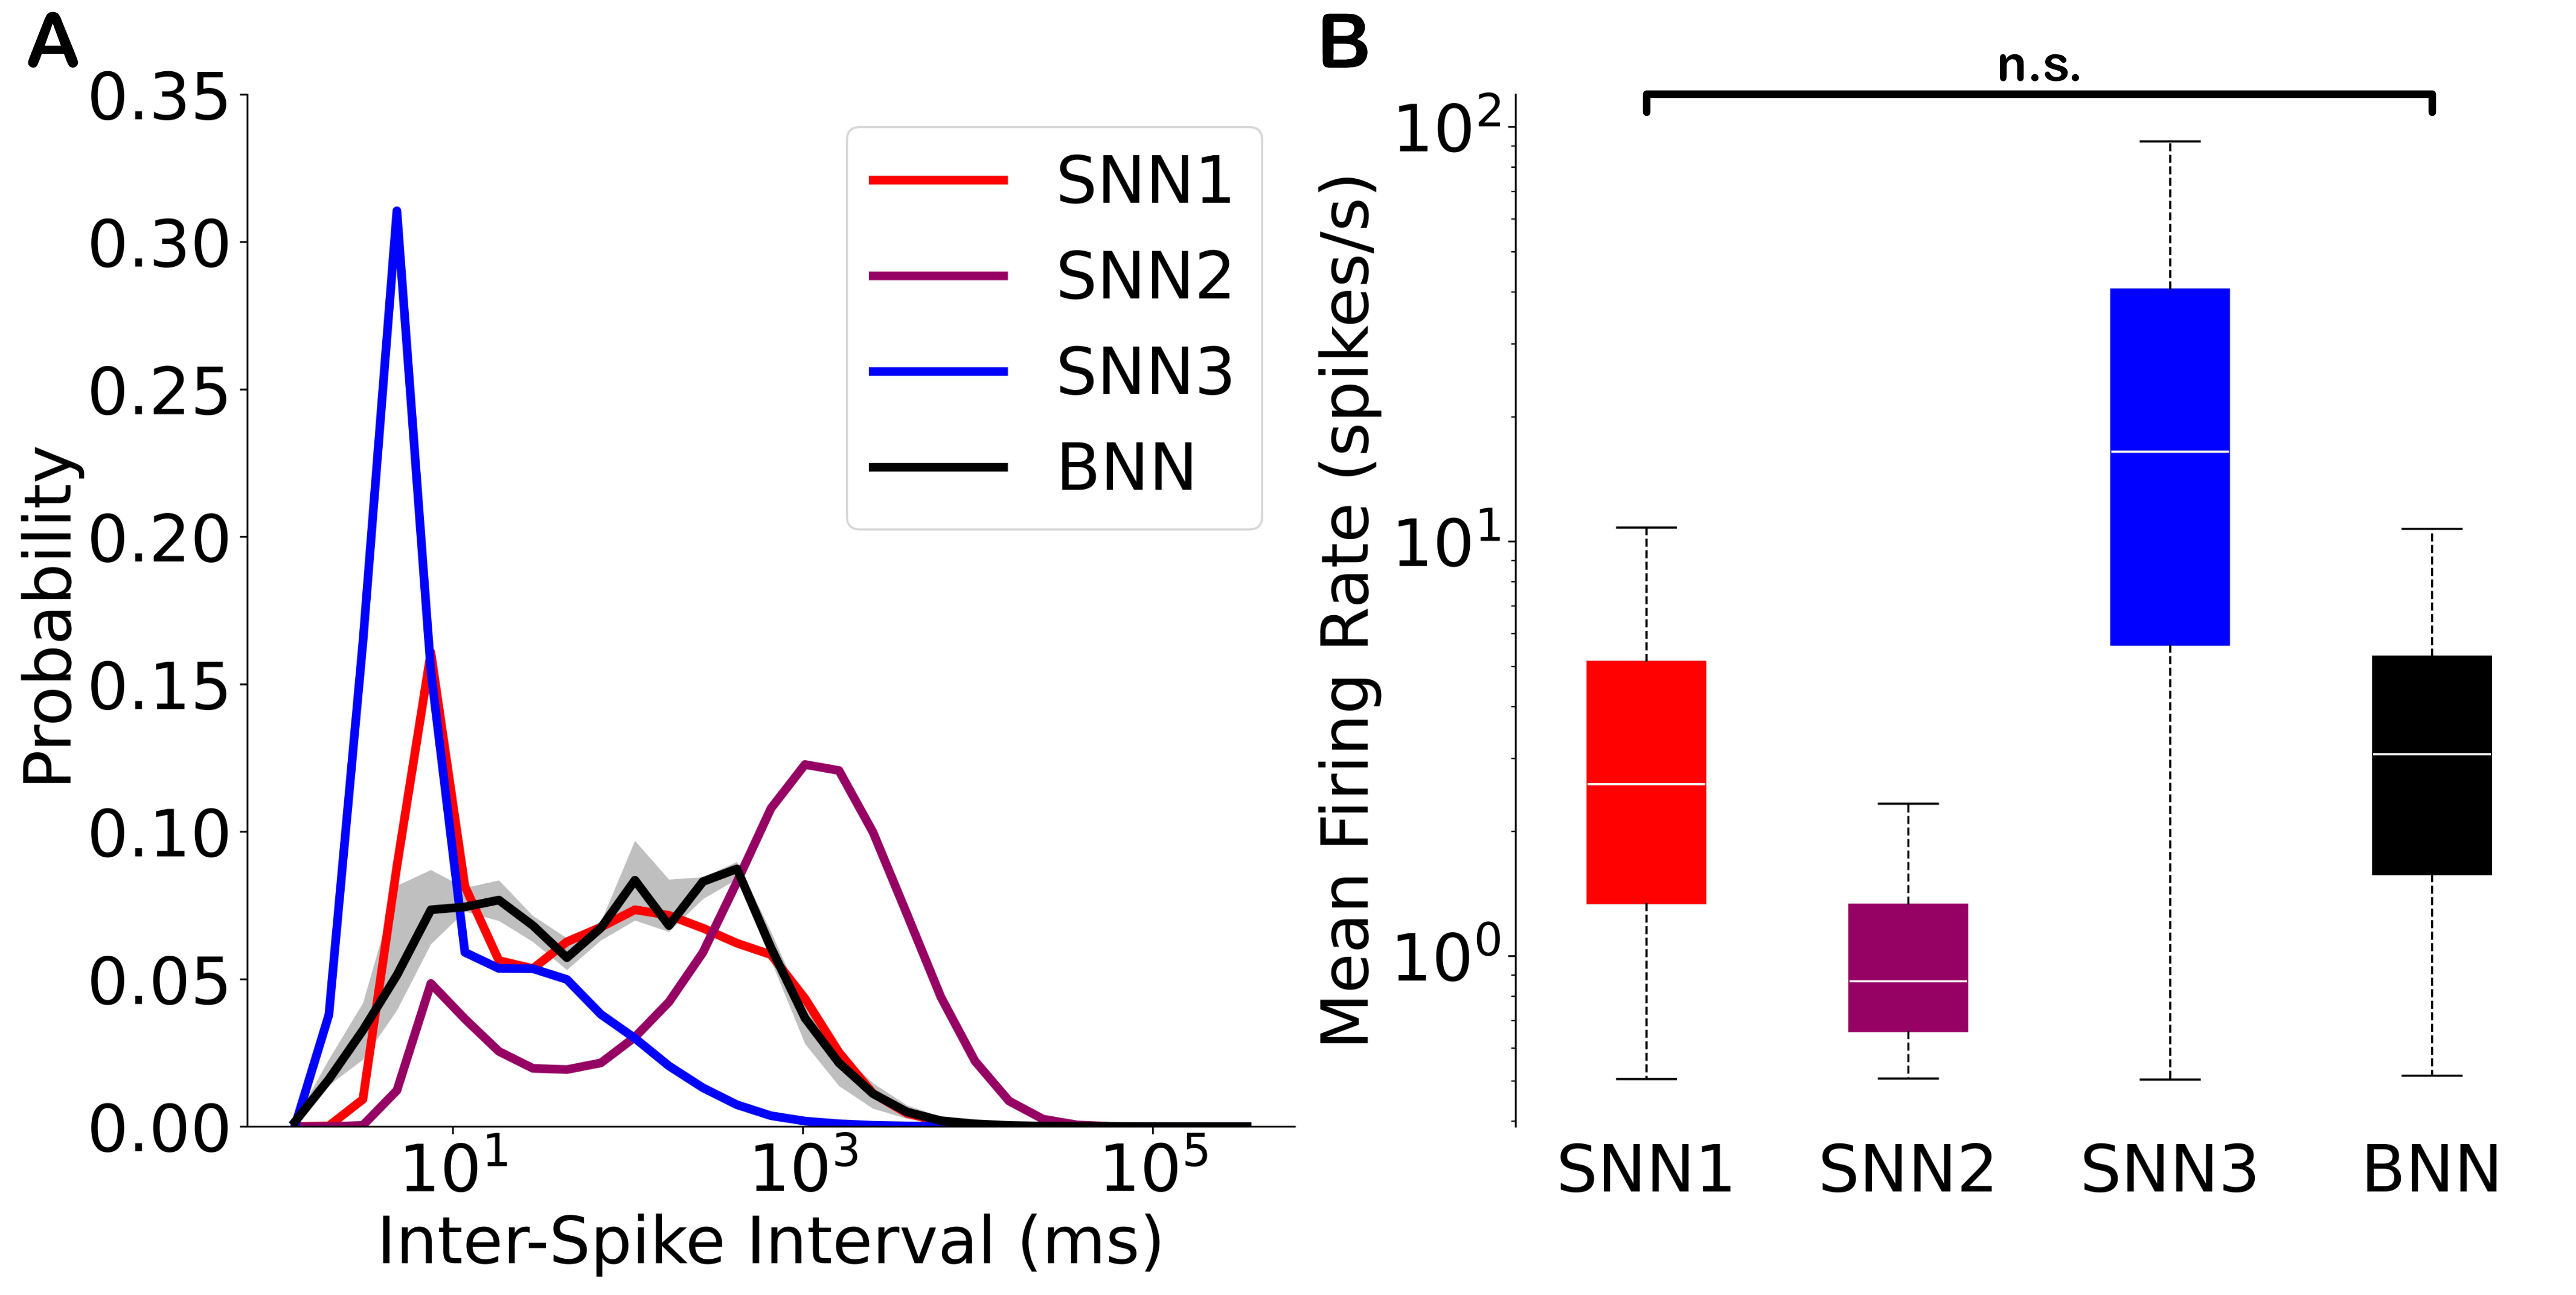
\includegraphics[width=\linewidth]{Figure/Histo-Box Comparison SNN-BNN.jpg}
    \end{center}
    \caption{Comparative analysis between BNNs and SNNs. (A) Inter Spike Interval Histograms (ISIHs) of three SNNs and the median trend of ISIHs from six selected rats. The shaded area denotes the range between the 25th and 75th percentiles. (B) MFR boxplots of all the single units in the three SNNs and the BNN. The BNN data were obtained by pooling together all single-unit activity of 6 rats. The central white line of the boxplots represents the median, while the top and bottom of the boxes are the 25-th and 75-th percentiles. The whiskers show the Q1-1.5*IQR and Q3+1.5*IQR, where Q1 and Q3 are the first and third quartiles, while the IQR is the interquartile range.}
    \label{fig:Histo-Box Comparison SNN-BNN}
\end{figure}

A first, qualitative evaluation indicates a good match between SNN1 and the pool of BNNs, which deviates from the profile of both SNN2 and SNN3. This is in accordance with the scores obtained in Table \ref{tab:Network Performance}, indicating SNN1 as the configuration better resembling the activity of the in vivo biological network. This is also confirmed by statistical analysis performed on the firing rate (Figure \ref{fig:Histo-Box Comparison SNN-BNN}B), for which SNN1 values do not significantly differ from those of the BNNs ($p= 0.477$, one-way ANOVA). For all the other network comparisons, the null hypothesis was rejected ($p<0.0001$, one-way ANOVA Figure \ref{fig:Histo-Box Comparison SNN-BNN}B). 

Furthermore, the raster plots presented in Figure \ref{fig:Raster Comparison SNN-BNN} offer a clear, even if qualitative, representation of the obtained electrophysiological activity for the optimal SNN (i.e. SNN1), the low-scored SNN2 and SNN3 and one representative in vivo network from rat. Indeed, SNN1 is the one better resembling the spike pattern of the BNN.

\begin{figure}[ht!]
    \begin{center}
    \includegraphics[width=\linewidth]{Figure/Raster Comparison SNN-BNN.jpg}
    \end{center}
    \caption{Comparative analysis between BNNs and SNNs. 20-s raster plot showing the firing activity of 30 neurons of each considered network.}
    \label{fig:Raster Comparison SNN-BNN}
\end{figure}

\section{Discussion and Conclusion}

In this study, a real-time Spiking Neural Network (SNN) was introduced to replicate key electrophysiological properties observed in an in vivo neuronal network. A dataset of six experiments on anesthetized rats was utilized to identify the target dynamics of the reference Biological Neural Network (BNN). Using BioemuS, a custom-developed FPGA-based platform containing 1024 single-compartment Hodgkin-Huxley neurons and 2\textsuperscript{20} synapses, simulations were conducted for 325 different SNNs. A procedure was developed to select the optimal SNN configuration capable of emulating the electrophysiological behavior of the BNN. The identified SNN exhibited primary biomarkers typical of in vivo cortical networks, such as firing and bursting rates, correlation levels, burstiness index, and Inter Spike Interval histogram. These results represent an important milestone for the future development of experiments where the SNN will drive the stimulation in vivo, paving the way for innovative neuromorphic-based neuroprostheses \cite{Chiappalone2022}.

\newpage
\phantomsection
\addcontentsline{toc}{chapter}{Conclusions and Future Perspectives}
\chapter*{Conclusions and Future Perspectives}

This thesis primarily aimed to advance the development of a novel neuromodulation technique, where the stimulation would be driven by a real-time hardware-based biomimetic SNN. Thus, the spontaneous activity of the RFA area of anesthetized rats, considered as the BNN, was analyzed to provide a target for fine-tuning the SNN, named Bi{\oe}muS. Key electrophysiological features of the in vivo neural network were successfully replicated by the SNN, such as firing and bursting rates, correlation levels, burstiness index, and inter-spike interval histogram. A total of 325 SNNs were simulated, and the one that best matched the characteristics observed in the target BNN was identified through a grading system based on a set of metrics that considered the similarity between the artificial and biological neural networks.

Regarding the design aspect of the SNN, in the future, an automatic tuning mechanism could be implemented to fine-tune its parameters, enabling a more accurate replication of the BNN behavior. Additionally, instead of utilizing an algorithm that arranges neurons in a cluster-like fashion, an approach that introduces scale-free or small-world properties to the network could be considered. All these details are essential for creating a highly personalized and biomimetic SNN that faithfully reproduces the dynamics of the targeted subject and can substitute a damaged brain region.

Furthermore, considering the future use of this platform for delivering personalized stimulation, the evoked activity in the RFA and S1 areas was also analyzed. In particular, the connectivity mapping phases were considered to compute the PSTH, enabling the understanding of how the lesion and traditional neuromodulation approaches affect the interplay between RFA and S1. It was possible to highlight a critical decrease in the evoked activity in the PoL phase, however, none of the OL techniques were able to bring the activity back to the level observed in the PreL phase. Once this technology is used for new in vivo experiments, it will be possible to assess the significance of such an open-loop technique, considering also its evoked results.

\newpage
\phantomsection
\addcontentsline{toc}{chapter}{Bibliography}
\nocite{*}
\bibliographystyle{namedn}
\bibliography{biblio}

\end{document}